\documentclass[titlepage]{article}

% Suppresses chktex warnings 
% chktex-file 1
% chktex-file 3
% chktex-file 8
% chktex-file 10
% chktex-file 11
% chktex-file 17
% chktex-file 24
% chktex-file 26
% chktex-file 36
% chktex-file 44
% chktex-file 46

\usepackage{geometry}
\usepackage{tikz}
\usetikzlibrary{fit}
\usetikzlibrary{positioning}
\usetikzlibrary{intersections}
\usetikzlibrary{matrix}
\usetikzlibrary{decorations.pathreplacing}
\usetikzlibrary{patterns}
\usetikzlibrary{3d}
\usetikzlibrary{arrows}
\usepackage{pgf}        % Used to import pgf figures with \input
\def\mathdefault#1{#1}  % Fixes 'Undefined control sequence \mathdefault' in imported pgf files
\usepackage{pgfplots}
\usepgfplotslibrary{fillbetween}
\pgfplotsset{compat=1.18}
\pgfplotsset{hide xscale/.style={/pgfplots/xtick scale label code/.code={}}}
\pgfplotsset{hide yscale/.style={/pgfplots/ytick scale label code/.code={}}}
\usepackage{amsmath}
\usepackage{upgreek}
\usepackage{url}
\hyphenation{}	        % Correct bad hyphenation
\usepackage{graphicx}   % For including figures and pictures
\usepackage{float}      % Used to fix location of images i.e.\begin{figure}[H]
\usepackage{fancyhdr}   % For headers and footers
\pagestyle{fancy}
\usepackage{lastpage}   % Allows referencing last page (for footer)
\usepackage{listings}   % For highlighting code
\usepackage{titling}    % To reference title, author, and date
\usepackage{array}      % For fixed-width tables
\usepackage{tabularx}   % For tables with automatic line breaks and fixed widths too i think
\usepackage{makecell}   % Formats individual table cells
\usepackage{multirow}   % For multi-row columns (Top left justify header)
\usepackage[american]{circuitikz} % Used to draw circuit and block diagrams
\usepackage{appendix}   
\usepackage{xcolor}     % For coloring code listings and other stuff probably
\usepackage{colortbl}   % For coloring table cells
\definecolor{nraoblue}{rgb}{0.776,0.851,0.945}  % Color of table headers
\usepackage{enumitem}   % For formatting enumerated lists
\usepackage[parfill]{parskip}               % Removes paragraph indentation, adds line break
\usepackage[hang, flushmargin]{footmisc}    % Removes footnote indentation
\setenumerate[1]{label={(\arabic*)}}
\usepackage[backend=biber,style=numeric,sorting=none]{biblatex}
\addbibresource{references.bib}
\usepackage{hyperref}   % Allows hyperlinks
\hypersetup{
  colorlinks   = true,  % Colors links instead of ugly boxes
  filecolor    = blue,  % Color for local hyperlinks
  linkcolor    = ., % Color for internal hyperlinks
  citecolor    = ., % Color for citations
  urlcolor     = blue,  % Color for linked urls
}
\usepackage{caption}    % Changes figure/table caption color and size
\usepackage{subcaption} % Allows multiple figures side by side
\definecolor{captioncolor}{RGB}{79,129,189}
\captionsetup{font={
    small, 
    color=captioncolor,
    bf,
}}

% Changes font from Computer Modern to Gill Sans MT
% This requires XeLaTeX or LuaTeX to function
% Add "latex-workshop.latex.recipe.default": "latexmk (xelatex)" to workspace.json
\usepackage{fontspec}
\setmainfont{gil.ttf}[
    BoldFont        = gil-b.ttf,
    ItalicFont      = gil-i.ttf,
    BoldItalicFont  = gil-bi.ttf,
]

% Code listing styling
\definecolor{codegreen}{rgb}{0,0.6,0}
\definecolor{codegray}{rgb}{0.5,0.5,0.5}
\definecolor{codepurple}{rgb}{0.58,0,0.82}
\definecolor{backcolour}{rgb}{0.95,0.95,0.92}
\lstdefinestyle{mystyle}{
    backgroundcolor=\color{backcolour},   
    commentstyle=\color{codegreen},
    keywordstyle=\color{magenta},
    numberstyle=\tiny\color{codegray},
    stringstyle=\color{codepurple},
    basicstyle=\ttfamily\footnotesize,
    breakatwhitespace=false,         
    breaklines=true,                 
    captionpos=b,                    
    keepspaces=true,                 
    numbers=left,                    
    numbersep=5pt,                  
    showspaces=false,                
    showstringspaces=false,
    showtabs=false,                  
    tabsize=2
}

\lstset{style=mystyle}
% Global TikZ parameters
\tikzset{every picture/.style={/utils/exec={\fontfamily{lmr}}}}
\ctikzset{sources/fill=red!20}
\ctikzset{chips/fill=cyan!20}
\ctikzset{electromechanicals/fill=blue!20}
\ctikzset{blocks/fill=green!20}
\ctikzset{amplifiers/fill=yellow!30}
\tikzset{amp/.append style={fill=yellow!30}}
\tikzset{twoport/.append style={fill=cyan!20}}
% TikZ hatch pattern used in trace cross section
\tikzset{
        hatch distance/.store in=\hatchdistance,
        hatch distance=3.5pt,
        hatch thickness/.store in=\hatchthickness,
        hatch thickness=0pt
    }
\makeatletter
\pgfdeclarepatternformonly[\hatchdistance,\hatchthickness]{flexible hatch}
    {\pgfqpoint{0pt}{0pt}}
    {\pgfqpoint{\hatchdistance}{\hatchdistance}}
    {\pgfpoint{\hatchdistance-1pt}{\hatchdistance-1pt}}%
    {
        \pgfsetcolor{\tikz@pattern@color}
        \pgfsetlinewidth{\hatchthickness}
        \pgfpathmoveto{\pgfqpoint{0.5pt}{0.5pt}}
        \pgfpathlineto{\pgfqpoint{\hatchdistance}{\hatchdistance}}
        \pgfusepath{stroke}
    }
\makeatother
% TikZ node[server] symbol
\makeatletter
\pgfkeys{/pgf/.cd,
  parallelepiped offset x/.initial=2mm,
  parallelepiped offset y/.initial=2mm
}
\pgfdeclareshape{parallelepiped}
{
  \inheritsavedanchors[from=rectangle] % this is nearly a rectangle
  \inheritanchorborder[from=rectangle]
  \inheritanchor[from=rectangle]{north}
  \inheritanchor[from=rectangle]{north west}
  \inheritanchor[from=rectangle]{north east}
  \inheritanchor[from=rectangle]{center}
  \inheritanchor[from=rectangle]{west}
  \inheritanchor[from=rectangle]{east}
  \inheritanchor[from=rectangle]{mid}
  \inheritanchor[from=rectangle]{mid west}
  \inheritanchor[from=rectangle]{mid east}
  \inheritanchor[from=rectangle]{base}
  \inheritanchor[from=rectangle]{base west}
  \inheritanchor[from=rectangle]{base east}
  \inheritanchor[from=rectangle]{south}
  \inheritanchor[from=rectangle]{south west}
  \inheritanchor[from=rectangle]{south east}
  \backgroundpath{
    % store lower right in xa/ya and upper right in xb/yb
    \southwest \pgf@xa=\pgf@x \pgf@ya=\pgf@y
    \northeast \pgf@xb=\pgf@x \pgf@yb=\pgf@y
    \pgfmathsetlength\pgfutil@tempdima{\pgfkeysvalueof{/pgf/parallelepiped
      offset x}}
    \pgfmathsetlength\pgfutil@tempdimb{\pgfkeysvalueof{/pgf/parallelepiped
      offset y}}
    \def\ppd@offset{\pgfpoint{\pgfutil@tempdima}{\pgfutil@tempdimb}}
    \pgfpathmoveto{\pgfqpoint{\pgf@xa}{\pgf@ya}}
    \pgfpathlineto{\pgfqpoint{\pgf@xb}{\pgf@ya}}
    \pgfpathlineto{\pgfqpoint{\pgf@xb}{\pgf@yb}}
    \pgfpathlineto{\pgfqpoint{\pgf@xa}{\pgf@yb}}
    \pgfpathclose
    \pgfpathmoveto{\pgfqpoint{\pgf@xb}{\pgf@ya}}
    \pgfpathlineto{\pgfpointadd{\pgfpoint{\pgf@xb}{\pgf@ya}}{\ppd@offset}}
    \pgfpathlineto{\pgfpointadd{\pgfpoint{\pgf@xb}{\pgf@yb}}{\ppd@offset}}
    \pgfpathlineto{\pgfpointadd{\pgfpoint{\pgf@xa}{\pgf@yb}}{\ppd@offset}}
    \pgfpathlineto{\pgfqpoint{\pgf@xa}{\pgf@yb}}
    \pgfpathmoveto{\pgfqpoint{\pgf@xb}{\pgf@yb}}
    \pgfpathlineto{\pgfpointadd{\pgfpoint{\pgf@xb}{\pgf@yb}}{\ppd@offset}}
  }
}
\makeatother
% I don't even remember what this does
\tikzset{
  ports/.style={
    line width=0.3pt,
    top color=gray!20,
    bottom color=gray!80
  },
  server/.style={
    parallelepiped,
    fill=white, draw,
    minimum width=0.35cm,
    minimum height=0.75cm,
    parallelepiped offset x=3mm,
    parallelepiped offset y=2mm,
    xscale=-1,
    path picture={
      \draw[top color=gray!5,bottom color=gray!40]
      (path picture bounding box.south west) rectangle 
      (path picture bounding box.north east);
      \coordinate (A-center) at ($(path picture bounding box.center)!0!(path
        picture bounding box.south)$);
      \coordinate (A-west) at ([xshift=-0.575cm]path picture bounding box.west);
      \draw[ports]([yshift=0.1cm]$(A-west)!0!(A-center)$)
        rectangle +(0.2,0.065);
      \draw[ports]([yshift=0.01cm]$(A-west)!0.085!(A-center)$)
        rectangle +(0.15,0.05);
      \fill[black]([yshift=-0.35cm]$(A-west)!-0.1!(A-center)$)
        rectangle +(0.235,0.0175);
      \fill[black]([yshift=-0.385cm]$(A-west)!-0.1!(A-center)$)
        rectangle +(0.235,0.0175);
      \fill[black]([yshift=-0.42cm]$(A-west)!-0.1!(A-center)$)
        rectangle +(0.235,0.0175);
    }  
  },
}
% Adds key for current tikz coordinate
\newcommand\currentpos{\the\tikz@lastxsaved,\the\tikz@lastysaved}
% Wiring diagram matrix stuff (syntax for jumping lines and block styles)
\tikzset{
    connect/.style args={(#1) to (#2) over #3 by #4}{
        insert path={
            \pgfextra{
                \pgfinterruptpath
                    \path [name path=userpath] (#1) -- (#2);
                    \path [name intersections={of=userpath and #3,by=overpoint}];
                \endpgfinterruptpath                
            }
            let \p1=($(#1)-(overpoint)$), \n1={veclen(\x1,\y1)}, 
                            \n2={atan2(\y1,\x1)}, \n3={abs(#4)}, \n4={#4>0 ?180:-180}  in 
                            (#1) -- ($(#1)!\n1-\n3!(overpoint)$) 
                            arc (\n2:\n2+\n4:\n3) -- (#2)
        }
    },
}
\tikzset{wire board/.style={
          matrix of nodes,
          row sep={17pt, between origins},
          nodes={anchor=center, minimum height=14pt} % set min height or else distance from matrix.north to first row will change depending on the content of the first row
          },
        wiresright/.style={
          column 1/.style={nodes={left}},
          column 2/.style={font=\bfseries},
          column 3/.style={nodes={above right}},
          },
        wiresboth/.style={
          column 1/.style={nodes={above left}},
          column 2/.style={font=\bfseries},
          column 4/.style={font=\bfseries},
          column 5/.style={nodes={above right}},
          },
        wiresleft/.style={
          column 1/.style={nodes={above left}},
          column 2/.style={font=\bfseries},
          column 3/.style={nodes={right}},
        },
}

% The following lines define a new command \nraocite that cites references in NRAO format RD0X by redefining \cite command to remove brackets. \nraoprecite includes a prenote.
\DeclareCiteCommand{\cite} [\mkbibemph{\emph{}}]
  {\usebibmacro{prenote}}
  {\usebibmacro{citeindex}%
   \printtext[bibhyperref]{\usebibmacro{cite}}}
  {\multicitedelim}
  {\usebibmacro{postnote}}
\DeclareCiteCommand*{\cite} [\mkbibemph\emph{}]
  {\usebibmacro{prenote}}
  {\usebibmacro{citeindex}
   \printtext[bibhyperref]{\usebibmacro{citeyear}}}
  {\multicitedelim}
  {\usebibmacro{postnote}}
\newcommand{\nraocite}[1]{[RD0\cite{#1}]}
\newcommand{\nraoprecite}[2][]{[RD0\cite{#2}{, #1}]}


% ASSIGN TITLE, AUTHOR, DATE, DOCUMENT NUMBER, STATUS, HERE
\title{Title goes here}
\author{Author
    }% <-this % stops a space
\date{Jan 1, 2000}
\def\docnum{DOC NUM}
\def\status{\textcolor{red}{DRAFT}}

% HEADERS AND FOOTERS
\renewcommand{\headrulewidth}{0pt}
\fancyheadoffset[L,R]{2cm}
\fancyhead[L]{\vspace{-1cm}
\includegraphics[width=2cm]{images/NRAO Logo Badge.png}}
\fancyhead[R]{
\renewcommand{\arraystretch}{1.4}
\renewcommand{\arrayrulewidth}{0.25pt}
\begin{tabular}{|w{l}{6.7cm}|w{l}{4.9cm}|w{l}{3.4cm}|}
    \hline
        \multirow[t]{2}{6.7cm}{\textit{\textbf{Title:}} \thetitle} &
        \textit{\textbf{Owner:}} \theauthor &
        \textit{\textbf{Date:}}  \thedate \\
            &   &   \\
    \hline
        \multicolumn{2}{|l|}{
            \textit{\textbf{NRAO Doc \#:}} \docnum  
        } &
        \textit{\textbf{Version:}} A \\
    \hline
\end{tabular}
}
\fancyfoot[C]{Page \textbf{\thepage} of \textbf{\pageref{LastPage}}}

 % DOCUMENT STARTS HERE
\begin{document}
\setlength{\leftmargin}{1in}        % Sets margin
\setlength{\rightmargin}{1in}       % Sets margin
\setlength{\voffset}{-1.2in}        % Moves header up
\setlength{\headheight}{3.5cm}      % Defines header height
\setlength{\textheight}{591pt}      % Extends text/body size down
\setlength{\footskip}{60pt}         % Defines gap between body and footer

\thispagestyle{fancy}
\begin{center}
     
\includegraphics[width=5cm]{images/NRAO Logo Badge.png} \\
     \vspace*{0.5cm}
     \textbf{\huge\thetitle} \\
     \vspace*{0.5cm}
     \large\docnum \\
     \Large Status: \status \\
     \vspace*{0.6cm} \large
     % FIRST TABLE HERE
     \begin{tabular}{|m{6.93cm}|m{4.5cm}|m{2cm}|} \hline
        \rowcolor{nraoblue}
        \textbf{Prepared By} & \textbf{Organization} & \textbf{Date} \\ \hline
        \makecell[l]{Author\\Title} & NRAO Electronics Div. & 1/1/2000 \\ 
        \hline
    \end{tabular} \\
    \vspace*{0.8cm}
    \begin{tabular}{|m{3cm}|m{3.5cm}|m{6.93cm}|} \hline
        \rowcolor{nraoblue}
        \textbf{Approvals} & \textbf{Organization} & \textbf{Signatures} \\ \hline
    \end{tabular}
    \renewcommand{\arraystretch}{2}
    % CONTENT OF SECOND TABLE HERE
    \begin{tabular}{|w{l}{3cm}|m{3.5cm}|m{6.93cm}|} \hline
        \parbox{3cm}{\raggedright
        Name\\Title
        } & NRAO Electronics Division \raggedright &  \\ 
        \hline
        \parbox{3cm}{\raggedright
        Name\\Title
        } & NRAO Electronics Division \raggedright &  \\ 
        \hline
        \parbox{3cm}{\raggedright
        Name\\Title
        } & NRAO Electronics Division \raggedright &  \\ 
        \hline
    \end{tabular} \\
    \renewcommand{\arraystretch}{1}
    \vspace*{0.8cm}
    \begin{tabular}{|m{3cm}|m{3.5cm}|m{6.93cm}|} \hline
        \rowcolor{nraoblue}
        \textbf{Released By} & \textbf{Organization} & \textbf{Signature} \\ \hline
    \end{tabular}
    \renewcommand{\arraystretch}{1.5}
    % CONTENT OF THIRD TABLE HERE
    \begin{tabular}{|m{3cm}|m{3.5cm}|m{6.93cm}|} \hline
        \parbox{3cm}{\raggedright
        Name\\Title
        } & NRAO Electronics Division \raggedright &  \\ 
        \hline
    \end{tabular}
    \renewcommand{\arraystretch}{1}
\end{center}

% CHANGE RECORD
\newpage
\section*{Change Record}
\begin{center}
\renewcommand{\arraystretch}{1.2}
    \begin{tabular}{|m{1.5cm}|m{2.2cm}|m{2.5cm}|m{1.7cm}|m{5cm}|} \hline
        \rowcolor{nraoblue}
        Version & Date & Author & Affected\newline Section(s) & Reason\\ \hline
    \end{tabular}
\renewcommand{\arraystretch}{1.6}
    \begin{tabular}{|m{1.5cm}|m{2.2cm}|m{2.5cm}|m{1.7cm}|m{5cm}|} \hline
        01 & Aug 15, 2023 & R. Nguyen & All & Initial Draft \\ \hline
        02 & Aug 16, 2023 & \makecell[l]{T. Anderson\\R. Nguyen} & All & Edits \\ \hline
        A  & Aug 16, 2023 & T. Anderson & All & Review \\ \hline
          &          &           &     &               \\ \hline
          &          &           &     &               \\ \hline
          &          &           &     &               \\ \hline
          &          &           &     &               \\ \hline
    \end{tabular}
\renewcommand{\arraystretch}{1} % Row separation for tables in the rest of document
\end{center}

\newpage
\tableofcontents
\listoffigures
\listoftables
\thispagestyle{fancy}
\newpage

% DOCUMENT STARTS HERE
\section{Introduction}

\subsection{What is the RF-DFS and RF-EMS?}
% copy from readme/wiki/plan or something
The Radio Frequency - Direction Finding System and Environmental Monitoring System are tools utilized by the NRAO-NM Interference Protection Group to identify and locate RF interference at the Very Large Array. The former is a 3-meter dish antenna with azimuth and elevation drives whereas the latter is a 50-foot tower with an omnidirectional club antenna. Both are connected to the RFI shack and controlled by a Python front end. This interface allows a user to control RF switching between both antennas and log data through a spectrum analyzer. 

\subsection{System Overview}
The three locations of note are the RFI shack, the RF-DFS dish, and the RF-EMS tower. A block diagram which shows the breakdown of major components and their connections is shown in Figure~\ref{fig:sysblock2}. The user will be able to control all IO functions through the Python application run on the PC (\verb|EMSMONPC2|).  SCPI commands issued over GPIB allow the user to control and view the spectrum analyzer display on the PC and a serial connection facilitates the same function with the motor controller. This motor controller is a Parker Hannifin ACR9000 which drives 2 Aries AR-04AE servos; one each for azimuth and elevation. RF switching is controlled by a PLC in the RFI shack (not shown).

\begin{figure}[!h]
  \begin{center}
      \begin{circuitikz}
          % Shack
          \draw(0, 0) node[server, scale=1.5, name=computer]{};
          % \draw(computer.east) ++ (0.5, 0.2) node[anchor=west](computerlabel){PC};
          \draw(computer.west) node[anchor=east]{};
          \ctikzset{bipoles/oscope/waveform=triangle}
          \ctikzset{bipoles/oscope/width=1.0}
          \draw(computer.west)  ++ (-1, 0.2) 
          coordinate(ctrwest)-- ++ (-1.2, 0)
          node[oscopeshape, anchor=east](spec){};
          \draw(spec.west) -- ++ (-1.2, 0)
          node[twoportshape, anchor=east](shackswitch){};
          \draw(shackswitch.center) node[spdt, scale=0.6, xscale=-1]{};
          \draw(ctrwest) ++ (-0.6, 0) node[anchor=south]{GPIB};
          \draw(spec.south) node[anchor=north]{N9040b};
          \draw(spec.in 1) node[ocirc, scale=0.7]{};
          \draw(spec.in 2) node[ocirc, scale=0.7]{};
          \draw(spec.west) ++ (-0.6, 0) node[anchor=south]{Coax};

          % DFS
          \draw(shackswitch.west) -- ++ (-2, 0)
          to[amp, invert] ++ (-2, 0)
          to[amp, invert, name=dfslna1] ++ (-2, 0)
          -| ++ (-1, 0)
          coordinate(dfs)
          -- ++ (0, 0.5)
          node[bareantenna, anchor=south](dfsantenna){};
          % \draw(dfslna1.east) ++ (0.5, 0.5) node[anchor=south](){PMA3-14LN+};

          % EMS
          % \draw(spec.north) -- ++ (0, 1.5)
          % to[amp, invert, name=emslna2] ++ (0, 2)
          % to[amp, invert, name=emslna1] ++ (0, 2)
          % node[bareantenna, anchor=south](emsantenna){};
          \draw(shackswitch.north) -- ++ (0, 2)
          node[twoportshape, name=s1]{} -- ++ (0, 0.8)
          to[amp, boxed, invert] ++ (0, 1) -- ++ (0, 0.8)
          node[twoportshape, name=s2]{} -- ++ (0, 0.8)
          node[bareantenna, anchor=south](emsantenna){};
          % \draw(spec.north) ++ (0, 0.75) node[anchor=west]{Coax};
          \draw(s1.center) node[spdt, scale=0.6, rotate=90]{};
          \draw(s2.center) node[spdt, xscale=-1, scale=0.6, rotate=270]{};
          % \draw(emslna1) ++ (0, -0.7) node[anchor=west](emslnalabel){PMA3-14LN+};

          % Motor stuff
          \draw(computer.south) |- ++ (-8.5, -1)
          node[qfpchip, anchor=west, external pins width=0, hide numbers, name=acr, scale=0.8, align=center]{Motor\\Ctrl.};
          \draw(computer.south) ++ (0, -1)
          node[anchor=south east](seriallabel){RS-485};
          \draw([yshift=-8pt]acr.west) -- ++ (-2, 0)
          node[elmech, rotate=90, anchor=bottom](m2){};
          \draw(m2) [->, dashed] -| ([yshift=-10pt]dfs.center);
          \draw([yshift=8pt]acr.west) -- ++ (-0.6, 0)
          node[elmech, rotate=90, anchor=bottom](m1){};
          %\draw(m1) [->] -- ++ (3, 0) -- ([yshift=-10pt, xshift=-10pt]dfs.center);
          \path[name path = border3](dfs.center) -- ++ (0, -2);
          \path[name path = line3, overlay](m1.top) -- ++ (-5, 0);
          \draw[name intersections={of=border3 and line3}, dashed] (m1.top) -- (intersection-1)
          node[diamondpole]{};
          \draw(m1.center) node{Az};
          \draw(m2.center) node{El};

          % Boxes
          \node[draw, rectangle, dashed, fit=(dfsantenna) (acr), inner sep=10](dfsbox){};
          \node[draw, rectangle, dashed, fit=(emsantenna) (s1), inner sep=10](emsbox){};
          \node[draw, rectangle, dashed, fit=(shackswitch) (computer), inner sep=10](shackbox){};

          % Box Labels
          \draw(dfsbox.north) node[anchor=south]{RF - DFS};
          \draw(emsbox.west) node[anchor=east]{RF - EMS};
          \draw(shackbox.north east) node[anchor=south east]{RFI Shack};
      \end{circuitikz}
  \caption{System Block Diagram.}\label{fig:sysblock2}
  \end{center}
\end{figure}

\subsection{Proactive and Reactive Spectrum Monitoring}
There are two primary use cases for this system, the first is to proactively make records of the spectrum on a regular basis. These will be uploaded to DRIFT (described in Section~\ref{sec:drift}) and can be configured to be recorded at a time basis of the operator's will. The goal of this is to provide a substantial repository of spectral information that can be referenced at a later date when RFI in the VLA science data needs to be investigated.

When RFI needs to be examined at greater granularity, either in time, frequency, spectral resolution, or otherwise, the operator can manually configure spectrum analyzer parameters and save traces to the local machine. If the user is inside the RFI shack and not accessing the system remotely, they will also have full access to the spectrum analyzer features beyond those implemented in the Python interface.

\subsection{RF Signal Chain}\label{sec:rfchain}
Each system has a single 50-10000 MHz receiver but the framework is in place to add additional receivers relatively easily. Figure~\ref{fig:rfblock} shows an RF block diagram of existing components and the plan for an additional 6-18 GHz receiver on the EMS tower.

All switches are Dynatech Microwave M4-413K201L SP4T relay switches. Switches S2 and S3 are already installed in the EMS tower to make adding a receiver as streamlined as possible. The reason there are no switches at the DFS is because it requires either a redesign of the LNA housing to fit relay switches or solid state switches that are integrated on a board with the other RF components.

The coaxial cables running up the tower and to the dish are Andrew LDF1-50 1/4'' heliax cables with an upper frequency limit of 15800 MHz. The loss is around 21 dB/100ft at 16 GHz, as such, it may be required to build a downconverting stage for any higher frequency receivers, especially with the relatively long cable runs present in these systems. For reference, the mule tape measurement from conduit box to conduit box at the shack and RF-DFS is 120ft; the cable length from the shack to the RF-EMS was not measured but is noted to be 62ft in the 2001 RF-EMS senior design report.

The LNAs in these initial 50-10000 MHz receivers are Mini-Circuits PMA3-14LN+ wideband low noise MMICs. The boards that house these amplifiers are designed in house and fabricated on OSHPark 4-layer stackups in order to save cost over using prebuilt components. Figure~\ref{fig:pma3} shows the measured gain of an assembled amplifier over the operating frequency.

\begin{figure}[ht]
    \begin{center}
        \begin{circuitikz}
            % \draw[help lines, dashed] grid (14, 3);
            % \draw[help lines, dashed] grid (14, -3);

            \draw(0, 0) node[bnc](port1){N9040b};
            \draw(port1.hot) -- ++ (1, 0)
            node[rotary switch = 4 in 60 wiper 60, anchor=in](sw1){};
            
            \draw(sw1.out 1) -- ++ (0.75, 0) 
            to[twoport, name=emscableloss, fill=green!20] ++ (0, 2.75)
            -- ++ (0.75, 0)
            node[rotary switch = 4 in 60 wiper 60, anchor=in](sw2){};
            \draw (emscableloss.center) node[resistorshape, anchor = center, rotate = 90, scale = 0.8]{};
            
            % EMS low band
            \draw(sw2.out 1) -| ++ (1, 0.5) coordinate(abcd)
            -- ++ (0.5, 0)
            to[amp, invert, t=\ctikzflipx{\footnotesize LNA}] ++ (2.75, 0)
            coordinate(emsref1)
            to[amp, invert, t=\ctikzflipx{\footnotesize LNA}] ++ (2.75, 0)
            -- ++ (0.5, 0)
            coordinate(p1);
            
            % EMS downconverted stage
            \draw(sw2.out 2) -- (current subpath start -| abcd)
            -- ++ (0, -0.75)
            coordinate(asdf)
            -- ++ (0.25 ,0)
            to[amp, invert, name=ifamp, t=\ctikzflipx{IF}] ++ (1.5, 0)
            -- ++ (0.25, 0) node[mixer, anchor=w, name=mixer1, fill=cyan!20]{};
            \draw(mixer1.e) -- ++ (0.25, 0)
            to[bandpass] ++ (1.5, 0)
            to[amp, invert, name=rfamp, t=\ctikzflipx{RF}] ++ (1.5, 0) -- ++ (0.25, 0)
            coordinate(p2);
            \draw(mixer1.s)[<-] -- ++ (0, -0.5)
            node[oscillator, anchor=north, fill=cyan!20](pll){LO};
            
            % DFS
            \draw(sw1.out 2) -| ++ (0.5, 0)
            to[twoport, name=dfscableloss, fill=green!20] (current subpath start -| asdf)
            -- (current subpath start -| p2)
            node[ampshape, xscale=-1, anchor=east, fill=yellow!30, t=\ctikzflipx{\footnotesize LNA}](dfsref1){};
            \draw(dfsref1.west)
            to[amp, invert, t=\ctikzflipx{\footnotesize LNA}] ++ (2, 0)
            node[bnc, xscale=-1](port3){\ctikzflipx{DFS}};
            \draw (dfscableloss.center) node[resistorshape, anchor = center, rotate = 90, scale = 0.8]{};
            
            % EMS port
            \draw(sw2 -| p1) ++ (1, 0)
            node[rotary switch = 4 in 60 wiper 60, xscale=-1](sw3){};
            \draw(sw3.out 1) -| (p1);
            \draw(sw3.out 2) -| (p2);
            \draw(sw3.in) -- (sw3.in -| port3)
            node[bnc, xscale=-1](port2){\ctikzflipx{EMS}};

            % Switch labels and arrows
            \draw(sw1.north) node[anchor=south](sw1lab){S1};
            \draw(sw2.north) node[anchor=south](sw2lab){S2};
            \draw(sw3.north) node[anchor=south](sw3lab){S3};
            \draw(sw1lab.north) [dashed, <-] -- ++ (0, 3.5) coordinate(sw1plclabel) node[anchor=south]{PLC};
            \draw(sw2lab.north) [dashed, <-] -- (sw2lab.north |- sw1plclabel) node[anchor=south]{PLC};
            \draw(sw3lab.north) [dashed, <-] -- (sw3lab.north |- sw1plclabel) node[anchor=south]{PLC};

            % Phase 3 box            
            \node[draw, rectangle, dashed, fit=(ifamp) (rfamp) (pll), inner sep=8](ph3box){};

            % Labels
            \draw([yshift=2pt]dfscableloss.north)[<-] -- ++ (0, 0.15) node[anchor=south](cablelosslabel){Cable loss};
            \draw(cablelosslabel.north)[->] to [bend right=45] ([xshift=2pt]emscableloss.south);
            \draw(ph3box.south east) node[anchor=south east]{Future Upgrade};
            % \draw(emsref1.north |- sw1plclabel) node[anchor=south]{PMA3-14LN+};
            % \draw(dfsref1.north) ++ (0.8, 0.2) node[anchor=south]{PMA3-14LN+};
        \end{circuitikz}
    \caption{RF Block Diagram with Phase 3 Upgrades Shown.}\label{fig:rfblock}
    \end{center}
\end{figure}
\begin{figure}
  \begin{center}
      %% Creator: Matplotlib, PGF backend
%%
%% To include the figure in your LaTeX document, write
%%   \input{<filename>.pgf}
%%
%% Make sure the required packages are loaded in your preamble
%%   \usepackage{pgf}
%%
%% Also ensure that all the required font packages are loaded; for instance,
%% the lmodern package is sometimes necessary when using math font.
%%   \usepackage{lmodern}
%%
%% Figures using additional raster images can only be included by \input if
%% they are in the same directory as the main LaTeX file. For loading figures
%% from other directories you can use the `import` package
%%   \usepackage{import}
%%
%% and then include the figures with
%%   \import{<path to file>}{<filename>.pgf}
%%
%% Matplotlib used the following preamble
%%   \def\mathdefault#1{#1}
%%   \everymath=\expandafter{\the\everymath\displaystyle}
%%   
%%   \ifdefined\pdftexversion\else  % non-pdftex case.
%%     \usepackage{fontspec}
%%   \fi
%%   \makeatletter\@ifpackageloaded{underscore}{}{\usepackage[strings]{underscore}}\makeatother
%%
\begingroup%
\makeatletter%
\begin{pgfpicture}%
\pgfpathrectangle{\pgfpointorigin}{\pgfqpoint{4.800000in}{3.600000in}}%
\pgfusepath{use as bounding box, clip}%
\begin{pgfscope}%
\pgfsetbuttcap%
\pgfsetmiterjoin%
\definecolor{currentfill}{rgb}{1.000000,1.000000,1.000000}%
\pgfsetfillcolor{currentfill}%
\pgfsetlinewidth{0.000000pt}%
\definecolor{currentstroke}{rgb}{1.000000,1.000000,1.000000}%
\pgfsetstrokecolor{currentstroke}%
\pgfsetdash{}{0pt}%
\pgfpathmoveto{\pgfqpoint{0.000000in}{0.000000in}}%
\pgfpathlineto{\pgfqpoint{4.800000in}{0.000000in}}%
\pgfpathlineto{\pgfqpoint{4.800000in}{3.600000in}}%
\pgfpathlineto{\pgfqpoint{0.000000in}{3.600000in}}%
\pgfpathlineto{\pgfqpoint{0.000000in}{0.000000in}}%
\pgfpathclose%
\pgfusepath{fill}%
\end{pgfscope}%
\begin{pgfscope}%
\pgfsetbuttcap%
\pgfsetmiterjoin%
\definecolor{currentfill}{rgb}{1.000000,1.000000,1.000000}%
\pgfsetfillcolor{currentfill}%
\pgfsetlinewidth{0.000000pt}%
\definecolor{currentstroke}{rgb}{0.000000,0.000000,0.000000}%
\pgfsetstrokecolor{currentstroke}%
\pgfsetstrokeopacity{0.000000}%
\pgfsetdash{}{0pt}%
\pgfpathmoveto{\pgfqpoint{0.435417in}{0.423750in}}%
\pgfpathlineto{\pgfqpoint{4.416667in}{0.423750in}}%
\pgfpathlineto{\pgfqpoint{4.416667in}{3.338250in}}%
\pgfpathlineto{\pgfqpoint{0.435417in}{3.338250in}}%
\pgfpathlineto{\pgfqpoint{0.435417in}{0.423750in}}%
\pgfpathclose%
\pgfusepath{fill}%
\end{pgfscope}%
\begin{pgfscope}%
\pgfpathrectangle{\pgfqpoint{0.435417in}{0.423750in}}{\pgfqpoint{3.981250in}{2.914500in}}%
\pgfusepath{clip}%
\pgfsetrectcap%
\pgfsetroundjoin%
\pgfsetlinewidth{0.803000pt}%
\definecolor{currentstroke}{rgb}{0.690196,0.690196,0.690196}%
\pgfsetstrokecolor{currentstroke}%
\pgfsetdash{}{0pt}%
\pgfpathmoveto{\pgfqpoint{0.435417in}{0.423750in}}%
\pgfpathlineto{\pgfqpoint{0.435417in}{3.338250in}}%
\pgfusepath{stroke}%
\end{pgfscope}%
\begin{pgfscope}%
\pgfsetbuttcap%
\pgfsetroundjoin%
\definecolor{currentfill}{rgb}{0.000000,0.000000,0.000000}%
\pgfsetfillcolor{currentfill}%
\pgfsetlinewidth{0.803000pt}%
\definecolor{currentstroke}{rgb}{0.000000,0.000000,0.000000}%
\pgfsetstrokecolor{currentstroke}%
\pgfsetdash{}{0pt}%
\pgfsys@defobject{currentmarker}{\pgfqpoint{0.000000in}{-0.048611in}}{\pgfqpoint{0.000000in}{0.000000in}}{%
\pgfpathmoveto{\pgfqpoint{0.000000in}{0.000000in}}%
\pgfpathlineto{\pgfqpoint{0.000000in}{-0.048611in}}%
\pgfusepath{stroke,fill}%
}%
\begin{pgfscope}%
\pgfsys@transformshift{0.435417in}{0.423750in}%
\pgfsys@useobject{currentmarker}{}%
\end{pgfscope}%
\end{pgfscope}%
\begin{pgfscope}%
\definecolor{textcolor}{rgb}{0.000000,0.000000,0.000000}%
\pgfsetstrokecolor{textcolor}%
\pgfsetfillcolor{textcolor}%
\pgftext[x=0.435417in,y=0.326527in,,top]{\color{textcolor}{\rmfamily\fontsize{10.000000}{12.000000}\selectfont\catcode`\^=\active\def^{\ifmmode\sp\else\^{}\fi}\catcode`\%=\active\def%{\%}$\mathdefault{0}$}}%
\end{pgfscope}%
\begin{pgfscope}%
\pgfpathrectangle{\pgfqpoint{0.435417in}{0.423750in}}{\pgfqpoint{3.981250in}{2.914500in}}%
\pgfusepath{clip}%
\pgfsetrectcap%
\pgfsetroundjoin%
\pgfsetlinewidth{0.803000pt}%
\definecolor{currentstroke}{rgb}{0.690196,0.690196,0.690196}%
\pgfsetstrokecolor{currentstroke}%
\pgfsetdash{}{0pt}%
\pgfpathmoveto{\pgfqpoint{1.231667in}{0.423750in}}%
\pgfpathlineto{\pgfqpoint{1.231667in}{3.338250in}}%
\pgfusepath{stroke}%
\end{pgfscope}%
\begin{pgfscope}%
\pgfsetbuttcap%
\pgfsetroundjoin%
\definecolor{currentfill}{rgb}{0.000000,0.000000,0.000000}%
\pgfsetfillcolor{currentfill}%
\pgfsetlinewidth{0.803000pt}%
\definecolor{currentstroke}{rgb}{0.000000,0.000000,0.000000}%
\pgfsetstrokecolor{currentstroke}%
\pgfsetdash{}{0pt}%
\pgfsys@defobject{currentmarker}{\pgfqpoint{0.000000in}{-0.048611in}}{\pgfqpoint{0.000000in}{0.000000in}}{%
\pgfpathmoveto{\pgfqpoint{0.000000in}{0.000000in}}%
\pgfpathlineto{\pgfqpoint{0.000000in}{-0.048611in}}%
\pgfusepath{stroke,fill}%
}%
\begin{pgfscope}%
\pgfsys@transformshift{1.231667in}{0.423750in}%
\pgfsys@useobject{currentmarker}{}%
\end{pgfscope}%
\end{pgfscope}%
\begin{pgfscope}%
\definecolor{textcolor}{rgb}{0.000000,0.000000,0.000000}%
\pgfsetstrokecolor{textcolor}%
\pgfsetfillcolor{textcolor}%
\pgftext[x=1.231667in,y=0.326527in,,top]{\color{textcolor}{\rmfamily\fontsize{10.000000}{12.000000}\selectfont\catcode`\^=\active\def^{\ifmmode\sp\else\^{}\fi}\catcode`\%=\active\def%{\%}$\mathdefault{2000}$}}%
\end{pgfscope}%
\begin{pgfscope}%
\pgfpathrectangle{\pgfqpoint{0.435417in}{0.423750in}}{\pgfqpoint{3.981250in}{2.914500in}}%
\pgfusepath{clip}%
\pgfsetrectcap%
\pgfsetroundjoin%
\pgfsetlinewidth{0.803000pt}%
\definecolor{currentstroke}{rgb}{0.690196,0.690196,0.690196}%
\pgfsetstrokecolor{currentstroke}%
\pgfsetdash{}{0pt}%
\pgfpathmoveto{\pgfqpoint{2.027917in}{0.423750in}}%
\pgfpathlineto{\pgfqpoint{2.027917in}{3.338250in}}%
\pgfusepath{stroke}%
\end{pgfscope}%
\begin{pgfscope}%
\pgfsetbuttcap%
\pgfsetroundjoin%
\definecolor{currentfill}{rgb}{0.000000,0.000000,0.000000}%
\pgfsetfillcolor{currentfill}%
\pgfsetlinewidth{0.803000pt}%
\definecolor{currentstroke}{rgb}{0.000000,0.000000,0.000000}%
\pgfsetstrokecolor{currentstroke}%
\pgfsetdash{}{0pt}%
\pgfsys@defobject{currentmarker}{\pgfqpoint{0.000000in}{-0.048611in}}{\pgfqpoint{0.000000in}{0.000000in}}{%
\pgfpathmoveto{\pgfqpoint{0.000000in}{0.000000in}}%
\pgfpathlineto{\pgfqpoint{0.000000in}{-0.048611in}}%
\pgfusepath{stroke,fill}%
}%
\begin{pgfscope}%
\pgfsys@transformshift{2.027917in}{0.423750in}%
\pgfsys@useobject{currentmarker}{}%
\end{pgfscope}%
\end{pgfscope}%
\begin{pgfscope}%
\definecolor{textcolor}{rgb}{0.000000,0.000000,0.000000}%
\pgfsetstrokecolor{textcolor}%
\pgfsetfillcolor{textcolor}%
\pgftext[x=2.027917in,y=0.326527in,,top]{\color{textcolor}{\rmfamily\fontsize{10.000000}{12.000000}\selectfont\catcode`\^=\active\def^{\ifmmode\sp\else\^{}\fi}\catcode`\%=\active\def%{\%}$\mathdefault{4000}$}}%
\end{pgfscope}%
\begin{pgfscope}%
\pgfpathrectangle{\pgfqpoint{0.435417in}{0.423750in}}{\pgfqpoint{3.981250in}{2.914500in}}%
\pgfusepath{clip}%
\pgfsetrectcap%
\pgfsetroundjoin%
\pgfsetlinewidth{0.803000pt}%
\definecolor{currentstroke}{rgb}{0.690196,0.690196,0.690196}%
\pgfsetstrokecolor{currentstroke}%
\pgfsetdash{}{0pt}%
\pgfpathmoveto{\pgfqpoint{2.824167in}{0.423750in}}%
\pgfpathlineto{\pgfqpoint{2.824167in}{3.338250in}}%
\pgfusepath{stroke}%
\end{pgfscope}%
\begin{pgfscope}%
\pgfsetbuttcap%
\pgfsetroundjoin%
\definecolor{currentfill}{rgb}{0.000000,0.000000,0.000000}%
\pgfsetfillcolor{currentfill}%
\pgfsetlinewidth{0.803000pt}%
\definecolor{currentstroke}{rgb}{0.000000,0.000000,0.000000}%
\pgfsetstrokecolor{currentstroke}%
\pgfsetdash{}{0pt}%
\pgfsys@defobject{currentmarker}{\pgfqpoint{0.000000in}{-0.048611in}}{\pgfqpoint{0.000000in}{0.000000in}}{%
\pgfpathmoveto{\pgfqpoint{0.000000in}{0.000000in}}%
\pgfpathlineto{\pgfqpoint{0.000000in}{-0.048611in}}%
\pgfusepath{stroke,fill}%
}%
\begin{pgfscope}%
\pgfsys@transformshift{2.824167in}{0.423750in}%
\pgfsys@useobject{currentmarker}{}%
\end{pgfscope}%
\end{pgfscope}%
\begin{pgfscope}%
\definecolor{textcolor}{rgb}{0.000000,0.000000,0.000000}%
\pgfsetstrokecolor{textcolor}%
\pgfsetfillcolor{textcolor}%
\pgftext[x=2.824167in,y=0.326527in,,top]{\color{textcolor}{\rmfamily\fontsize{10.000000}{12.000000}\selectfont\catcode`\^=\active\def^{\ifmmode\sp\else\^{}\fi}\catcode`\%=\active\def%{\%}$\mathdefault{6000}$}}%
\end{pgfscope}%
\begin{pgfscope}%
\pgfpathrectangle{\pgfqpoint{0.435417in}{0.423750in}}{\pgfqpoint{3.981250in}{2.914500in}}%
\pgfusepath{clip}%
\pgfsetrectcap%
\pgfsetroundjoin%
\pgfsetlinewidth{0.803000pt}%
\definecolor{currentstroke}{rgb}{0.690196,0.690196,0.690196}%
\pgfsetstrokecolor{currentstroke}%
\pgfsetdash{}{0pt}%
\pgfpathmoveto{\pgfqpoint{3.620417in}{0.423750in}}%
\pgfpathlineto{\pgfqpoint{3.620417in}{3.338250in}}%
\pgfusepath{stroke}%
\end{pgfscope}%
\begin{pgfscope}%
\pgfsetbuttcap%
\pgfsetroundjoin%
\definecolor{currentfill}{rgb}{0.000000,0.000000,0.000000}%
\pgfsetfillcolor{currentfill}%
\pgfsetlinewidth{0.803000pt}%
\definecolor{currentstroke}{rgb}{0.000000,0.000000,0.000000}%
\pgfsetstrokecolor{currentstroke}%
\pgfsetdash{}{0pt}%
\pgfsys@defobject{currentmarker}{\pgfqpoint{0.000000in}{-0.048611in}}{\pgfqpoint{0.000000in}{0.000000in}}{%
\pgfpathmoveto{\pgfqpoint{0.000000in}{0.000000in}}%
\pgfpathlineto{\pgfqpoint{0.000000in}{-0.048611in}}%
\pgfusepath{stroke,fill}%
}%
\begin{pgfscope}%
\pgfsys@transformshift{3.620417in}{0.423750in}%
\pgfsys@useobject{currentmarker}{}%
\end{pgfscope}%
\end{pgfscope}%
\begin{pgfscope}%
\definecolor{textcolor}{rgb}{0.000000,0.000000,0.000000}%
\pgfsetstrokecolor{textcolor}%
\pgfsetfillcolor{textcolor}%
\pgftext[x=3.620417in,y=0.326527in,,top]{\color{textcolor}{\rmfamily\fontsize{10.000000}{12.000000}\selectfont\catcode`\^=\active\def^{\ifmmode\sp\else\^{}\fi}\catcode`\%=\active\def%{\%}$\mathdefault{8000}$}}%
\end{pgfscope}%
\begin{pgfscope}%
\pgfpathrectangle{\pgfqpoint{0.435417in}{0.423750in}}{\pgfqpoint{3.981250in}{2.914500in}}%
\pgfusepath{clip}%
\pgfsetrectcap%
\pgfsetroundjoin%
\pgfsetlinewidth{0.803000pt}%
\definecolor{currentstroke}{rgb}{0.690196,0.690196,0.690196}%
\pgfsetstrokecolor{currentstroke}%
\pgfsetdash{}{0pt}%
\pgfpathmoveto{\pgfqpoint{4.416667in}{0.423750in}}%
\pgfpathlineto{\pgfqpoint{4.416667in}{3.338250in}}%
\pgfusepath{stroke}%
\end{pgfscope}%
\begin{pgfscope}%
\pgfsetbuttcap%
\pgfsetroundjoin%
\definecolor{currentfill}{rgb}{0.000000,0.000000,0.000000}%
\pgfsetfillcolor{currentfill}%
\pgfsetlinewidth{0.803000pt}%
\definecolor{currentstroke}{rgb}{0.000000,0.000000,0.000000}%
\pgfsetstrokecolor{currentstroke}%
\pgfsetdash{}{0pt}%
\pgfsys@defobject{currentmarker}{\pgfqpoint{0.000000in}{-0.048611in}}{\pgfqpoint{0.000000in}{0.000000in}}{%
\pgfpathmoveto{\pgfqpoint{0.000000in}{0.000000in}}%
\pgfpathlineto{\pgfqpoint{0.000000in}{-0.048611in}}%
\pgfusepath{stroke,fill}%
}%
\begin{pgfscope}%
\pgfsys@transformshift{4.416667in}{0.423750in}%
\pgfsys@useobject{currentmarker}{}%
\end{pgfscope}%
\end{pgfscope}%
\begin{pgfscope}%
\definecolor{textcolor}{rgb}{0.000000,0.000000,0.000000}%
\pgfsetstrokecolor{textcolor}%
\pgfsetfillcolor{textcolor}%
\pgftext[x=4.416667in,y=0.326527in,,top]{\color{textcolor}{\rmfamily\fontsize{10.000000}{12.000000}\selectfont\catcode`\^=\active\def^{\ifmmode\sp\else\^{}\fi}\catcode`\%=\active\def%{\%}$\mathdefault{10000}$}}%
\end{pgfscope}%
\begin{pgfscope}%
\pgfsetbuttcap%
\pgfsetroundjoin%
\definecolor{currentfill}{rgb}{0.000000,0.000000,0.000000}%
\pgfsetfillcolor{currentfill}%
\pgfsetlinewidth{0.602250pt}%
\definecolor{currentstroke}{rgb}{0.000000,0.000000,0.000000}%
\pgfsetstrokecolor{currentstroke}%
\pgfsetdash{}{0pt}%
\pgfsys@defobject{currentmarker}{\pgfqpoint{0.000000in}{-0.027778in}}{\pgfqpoint{0.000000in}{0.000000in}}{%
\pgfpathmoveto{\pgfqpoint{0.000000in}{0.000000in}}%
\pgfpathlineto{\pgfqpoint{0.000000in}{-0.027778in}}%
\pgfusepath{stroke,fill}%
}%
\begin{pgfscope}%
\pgfsys@transformshift{0.634479in}{0.423750in}%
\pgfsys@useobject{currentmarker}{}%
\end{pgfscope}%
\end{pgfscope}%
\begin{pgfscope}%
\pgfsetbuttcap%
\pgfsetroundjoin%
\definecolor{currentfill}{rgb}{0.000000,0.000000,0.000000}%
\pgfsetfillcolor{currentfill}%
\pgfsetlinewidth{0.602250pt}%
\definecolor{currentstroke}{rgb}{0.000000,0.000000,0.000000}%
\pgfsetstrokecolor{currentstroke}%
\pgfsetdash{}{0pt}%
\pgfsys@defobject{currentmarker}{\pgfqpoint{0.000000in}{-0.027778in}}{\pgfqpoint{0.000000in}{0.000000in}}{%
\pgfpathmoveto{\pgfqpoint{0.000000in}{0.000000in}}%
\pgfpathlineto{\pgfqpoint{0.000000in}{-0.027778in}}%
\pgfusepath{stroke,fill}%
}%
\begin{pgfscope}%
\pgfsys@transformshift{0.833542in}{0.423750in}%
\pgfsys@useobject{currentmarker}{}%
\end{pgfscope}%
\end{pgfscope}%
\begin{pgfscope}%
\pgfsetbuttcap%
\pgfsetroundjoin%
\definecolor{currentfill}{rgb}{0.000000,0.000000,0.000000}%
\pgfsetfillcolor{currentfill}%
\pgfsetlinewidth{0.602250pt}%
\definecolor{currentstroke}{rgb}{0.000000,0.000000,0.000000}%
\pgfsetstrokecolor{currentstroke}%
\pgfsetdash{}{0pt}%
\pgfsys@defobject{currentmarker}{\pgfqpoint{0.000000in}{-0.027778in}}{\pgfqpoint{0.000000in}{0.000000in}}{%
\pgfpathmoveto{\pgfqpoint{0.000000in}{0.000000in}}%
\pgfpathlineto{\pgfqpoint{0.000000in}{-0.027778in}}%
\pgfusepath{stroke,fill}%
}%
\begin{pgfscope}%
\pgfsys@transformshift{1.032604in}{0.423750in}%
\pgfsys@useobject{currentmarker}{}%
\end{pgfscope}%
\end{pgfscope}%
\begin{pgfscope}%
\pgfsetbuttcap%
\pgfsetroundjoin%
\definecolor{currentfill}{rgb}{0.000000,0.000000,0.000000}%
\pgfsetfillcolor{currentfill}%
\pgfsetlinewidth{0.602250pt}%
\definecolor{currentstroke}{rgb}{0.000000,0.000000,0.000000}%
\pgfsetstrokecolor{currentstroke}%
\pgfsetdash{}{0pt}%
\pgfsys@defobject{currentmarker}{\pgfqpoint{0.000000in}{-0.027778in}}{\pgfqpoint{0.000000in}{0.000000in}}{%
\pgfpathmoveto{\pgfqpoint{0.000000in}{0.000000in}}%
\pgfpathlineto{\pgfqpoint{0.000000in}{-0.027778in}}%
\pgfusepath{stroke,fill}%
}%
\begin{pgfscope}%
\pgfsys@transformshift{1.430729in}{0.423750in}%
\pgfsys@useobject{currentmarker}{}%
\end{pgfscope}%
\end{pgfscope}%
\begin{pgfscope}%
\pgfsetbuttcap%
\pgfsetroundjoin%
\definecolor{currentfill}{rgb}{0.000000,0.000000,0.000000}%
\pgfsetfillcolor{currentfill}%
\pgfsetlinewidth{0.602250pt}%
\definecolor{currentstroke}{rgb}{0.000000,0.000000,0.000000}%
\pgfsetstrokecolor{currentstroke}%
\pgfsetdash{}{0pt}%
\pgfsys@defobject{currentmarker}{\pgfqpoint{0.000000in}{-0.027778in}}{\pgfqpoint{0.000000in}{0.000000in}}{%
\pgfpathmoveto{\pgfqpoint{0.000000in}{0.000000in}}%
\pgfpathlineto{\pgfqpoint{0.000000in}{-0.027778in}}%
\pgfusepath{stroke,fill}%
}%
\begin{pgfscope}%
\pgfsys@transformshift{1.629792in}{0.423750in}%
\pgfsys@useobject{currentmarker}{}%
\end{pgfscope}%
\end{pgfscope}%
\begin{pgfscope}%
\pgfsetbuttcap%
\pgfsetroundjoin%
\definecolor{currentfill}{rgb}{0.000000,0.000000,0.000000}%
\pgfsetfillcolor{currentfill}%
\pgfsetlinewidth{0.602250pt}%
\definecolor{currentstroke}{rgb}{0.000000,0.000000,0.000000}%
\pgfsetstrokecolor{currentstroke}%
\pgfsetdash{}{0pt}%
\pgfsys@defobject{currentmarker}{\pgfqpoint{0.000000in}{-0.027778in}}{\pgfqpoint{0.000000in}{0.000000in}}{%
\pgfpathmoveto{\pgfqpoint{0.000000in}{0.000000in}}%
\pgfpathlineto{\pgfqpoint{0.000000in}{-0.027778in}}%
\pgfusepath{stroke,fill}%
}%
\begin{pgfscope}%
\pgfsys@transformshift{1.828854in}{0.423750in}%
\pgfsys@useobject{currentmarker}{}%
\end{pgfscope}%
\end{pgfscope}%
\begin{pgfscope}%
\pgfsetbuttcap%
\pgfsetroundjoin%
\definecolor{currentfill}{rgb}{0.000000,0.000000,0.000000}%
\pgfsetfillcolor{currentfill}%
\pgfsetlinewidth{0.602250pt}%
\definecolor{currentstroke}{rgb}{0.000000,0.000000,0.000000}%
\pgfsetstrokecolor{currentstroke}%
\pgfsetdash{}{0pt}%
\pgfsys@defobject{currentmarker}{\pgfqpoint{0.000000in}{-0.027778in}}{\pgfqpoint{0.000000in}{0.000000in}}{%
\pgfpathmoveto{\pgfqpoint{0.000000in}{0.000000in}}%
\pgfpathlineto{\pgfqpoint{0.000000in}{-0.027778in}}%
\pgfusepath{stroke,fill}%
}%
\begin{pgfscope}%
\pgfsys@transformshift{2.226979in}{0.423750in}%
\pgfsys@useobject{currentmarker}{}%
\end{pgfscope}%
\end{pgfscope}%
\begin{pgfscope}%
\pgfsetbuttcap%
\pgfsetroundjoin%
\definecolor{currentfill}{rgb}{0.000000,0.000000,0.000000}%
\pgfsetfillcolor{currentfill}%
\pgfsetlinewidth{0.602250pt}%
\definecolor{currentstroke}{rgb}{0.000000,0.000000,0.000000}%
\pgfsetstrokecolor{currentstroke}%
\pgfsetdash{}{0pt}%
\pgfsys@defobject{currentmarker}{\pgfqpoint{0.000000in}{-0.027778in}}{\pgfqpoint{0.000000in}{0.000000in}}{%
\pgfpathmoveto{\pgfqpoint{0.000000in}{0.000000in}}%
\pgfpathlineto{\pgfqpoint{0.000000in}{-0.027778in}}%
\pgfusepath{stroke,fill}%
}%
\begin{pgfscope}%
\pgfsys@transformshift{2.426042in}{0.423750in}%
\pgfsys@useobject{currentmarker}{}%
\end{pgfscope}%
\end{pgfscope}%
\begin{pgfscope}%
\pgfsetbuttcap%
\pgfsetroundjoin%
\definecolor{currentfill}{rgb}{0.000000,0.000000,0.000000}%
\pgfsetfillcolor{currentfill}%
\pgfsetlinewidth{0.602250pt}%
\definecolor{currentstroke}{rgb}{0.000000,0.000000,0.000000}%
\pgfsetstrokecolor{currentstroke}%
\pgfsetdash{}{0pt}%
\pgfsys@defobject{currentmarker}{\pgfqpoint{0.000000in}{-0.027778in}}{\pgfqpoint{0.000000in}{0.000000in}}{%
\pgfpathmoveto{\pgfqpoint{0.000000in}{0.000000in}}%
\pgfpathlineto{\pgfqpoint{0.000000in}{-0.027778in}}%
\pgfusepath{stroke,fill}%
}%
\begin{pgfscope}%
\pgfsys@transformshift{2.625104in}{0.423750in}%
\pgfsys@useobject{currentmarker}{}%
\end{pgfscope}%
\end{pgfscope}%
\begin{pgfscope}%
\pgfsetbuttcap%
\pgfsetroundjoin%
\definecolor{currentfill}{rgb}{0.000000,0.000000,0.000000}%
\pgfsetfillcolor{currentfill}%
\pgfsetlinewidth{0.602250pt}%
\definecolor{currentstroke}{rgb}{0.000000,0.000000,0.000000}%
\pgfsetstrokecolor{currentstroke}%
\pgfsetdash{}{0pt}%
\pgfsys@defobject{currentmarker}{\pgfqpoint{0.000000in}{-0.027778in}}{\pgfqpoint{0.000000in}{0.000000in}}{%
\pgfpathmoveto{\pgfqpoint{0.000000in}{0.000000in}}%
\pgfpathlineto{\pgfqpoint{0.000000in}{-0.027778in}}%
\pgfusepath{stroke,fill}%
}%
\begin{pgfscope}%
\pgfsys@transformshift{3.023229in}{0.423750in}%
\pgfsys@useobject{currentmarker}{}%
\end{pgfscope}%
\end{pgfscope}%
\begin{pgfscope}%
\pgfsetbuttcap%
\pgfsetroundjoin%
\definecolor{currentfill}{rgb}{0.000000,0.000000,0.000000}%
\pgfsetfillcolor{currentfill}%
\pgfsetlinewidth{0.602250pt}%
\definecolor{currentstroke}{rgb}{0.000000,0.000000,0.000000}%
\pgfsetstrokecolor{currentstroke}%
\pgfsetdash{}{0pt}%
\pgfsys@defobject{currentmarker}{\pgfqpoint{0.000000in}{-0.027778in}}{\pgfqpoint{0.000000in}{0.000000in}}{%
\pgfpathmoveto{\pgfqpoint{0.000000in}{0.000000in}}%
\pgfpathlineto{\pgfqpoint{0.000000in}{-0.027778in}}%
\pgfusepath{stroke,fill}%
}%
\begin{pgfscope}%
\pgfsys@transformshift{3.222292in}{0.423750in}%
\pgfsys@useobject{currentmarker}{}%
\end{pgfscope}%
\end{pgfscope}%
\begin{pgfscope}%
\pgfsetbuttcap%
\pgfsetroundjoin%
\definecolor{currentfill}{rgb}{0.000000,0.000000,0.000000}%
\pgfsetfillcolor{currentfill}%
\pgfsetlinewidth{0.602250pt}%
\definecolor{currentstroke}{rgb}{0.000000,0.000000,0.000000}%
\pgfsetstrokecolor{currentstroke}%
\pgfsetdash{}{0pt}%
\pgfsys@defobject{currentmarker}{\pgfqpoint{0.000000in}{-0.027778in}}{\pgfqpoint{0.000000in}{0.000000in}}{%
\pgfpathmoveto{\pgfqpoint{0.000000in}{0.000000in}}%
\pgfpathlineto{\pgfqpoint{0.000000in}{-0.027778in}}%
\pgfusepath{stroke,fill}%
}%
\begin{pgfscope}%
\pgfsys@transformshift{3.421354in}{0.423750in}%
\pgfsys@useobject{currentmarker}{}%
\end{pgfscope}%
\end{pgfscope}%
\begin{pgfscope}%
\pgfsetbuttcap%
\pgfsetroundjoin%
\definecolor{currentfill}{rgb}{0.000000,0.000000,0.000000}%
\pgfsetfillcolor{currentfill}%
\pgfsetlinewidth{0.602250pt}%
\definecolor{currentstroke}{rgb}{0.000000,0.000000,0.000000}%
\pgfsetstrokecolor{currentstroke}%
\pgfsetdash{}{0pt}%
\pgfsys@defobject{currentmarker}{\pgfqpoint{0.000000in}{-0.027778in}}{\pgfqpoint{0.000000in}{0.000000in}}{%
\pgfpathmoveto{\pgfqpoint{0.000000in}{0.000000in}}%
\pgfpathlineto{\pgfqpoint{0.000000in}{-0.027778in}}%
\pgfusepath{stroke,fill}%
}%
\begin{pgfscope}%
\pgfsys@transformshift{3.819479in}{0.423750in}%
\pgfsys@useobject{currentmarker}{}%
\end{pgfscope}%
\end{pgfscope}%
\begin{pgfscope}%
\pgfsetbuttcap%
\pgfsetroundjoin%
\definecolor{currentfill}{rgb}{0.000000,0.000000,0.000000}%
\pgfsetfillcolor{currentfill}%
\pgfsetlinewidth{0.602250pt}%
\definecolor{currentstroke}{rgb}{0.000000,0.000000,0.000000}%
\pgfsetstrokecolor{currentstroke}%
\pgfsetdash{}{0pt}%
\pgfsys@defobject{currentmarker}{\pgfqpoint{0.000000in}{-0.027778in}}{\pgfqpoint{0.000000in}{0.000000in}}{%
\pgfpathmoveto{\pgfqpoint{0.000000in}{0.000000in}}%
\pgfpathlineto{\pgfqpoint{0.000000in}{-0.027778in}}%
\pgfusepath{stroke,fill}%
}%
\begin{pgfscope}%
\pgfsys@transformshift{4.018542in}{0.423750in}%
\pgfsys@useobject{currentmarker}{}%
\end{pgfscope}%
\end{pgfscope}%
\begin{pgfscope}%
\pgfsetbuttcap%
\pgfsetroundjoin%
\definecolor{currentfill}{rgb}{0.000000,0.000000,0.000000}%
\pgfsetfillcolor{currentfill}%
\pgfsetlinewidth{0.602250pt}%
\definecolor{currentstroke}{rgb}{0.000000,0.000000,0.000000}%
\pgfsetstrokecolor{currentstroke}%
\pgfsetdash{}{0pt}%
\pgfsys@defobject{currentmarker}{\pgfqpoint{0.000000in}{-0.027778in}}{\pgfqpoint{0.000000in}{0.000000in}}{%
\pgfpathmoveto{\pgfqpoint{0.000000in}{0.000000in}}%
\pgfpathlineto{\pgfqpoint{0.000000in}{-0.027778in}}%
\pgfusepath{stroke,fill}%
}%
\begin{pgfscope}%
\pgfsys@transformshift{4.217604in}{0.423750in}%
\pgfsys@useobject{currentmarker}{}%
\end{pgfscope}%
\end{pgfscope}%
\begin{pgfscope}%
\definecolor{textcolor}{rgb}{0.000000,0.000000,0.000000}%
\pgfsetstrokecolor{textcolor}%
\pgfsetfillcolor{textcolor}%
\pgftext[x=2.426042in,y=0.147639in,,top]{\color{textcolor}{\rmfamily\fontsize{10.000000}{12.000000}\selectfont\catcode`\^=\active\def^{\ifmmode\sp\else\^{}\fi}\catcode`\%=\active\def%{\%}Frequency (MHz)}}%
\end{pgfscope}%
\begin{pgfscope}%
\pgfpathrectangle{\pgfqpoint{0.435417in}{0.423750in}}{\pgfqpoint{3.981250in}{2.914500in}}%
\pgfusepath{clip}%
\pgfsetrectcap%
\pgfsetroundjoin%
\pgfsetlinewidth{0.803000pt}%
\definecolor{currentstroke}{rgb}{0.690196,0.690196,0.690196}%
\pgfsetstrokecolor{currentstroke}%
\pgfsetdash{}{0pt}%
\pgfpathmoveto{\pgfqpoint{0.435417in}{0.423750in}}%
\pgfpathlineto{\pgfqpoint{4.416667in}{0.423750in}}%
\pgfusepath{stroke}%
\end{pgfscope}%
\begin{pgfscope}%
\pgfsetbuttcap%
\pgfsetroundjoin%
\definecolor{currentfill}{rgb}{0.000000,0.000000,0.000000}%
\pgfsetfillcolor{currentfill}%
\pgfsetlinewidth{0.803000pt}%
\definecolor{currentstroke}{rgb}{0.000000,0.000000,0.000000}%
\pgfsetstrokecolor{currentstroke}%
\pgfsetdash{}{0pt}%
\pgfsys@defobject{currentmarker}{\pgfqpoint{-0.048611in}{0.000000in}}{\pgfqpoint{-0.000000in}{0.000000in}}{%
\pgfpathmoveto{\pgfqpoint{-0.000000in}{0.000000in}}%
\pgfpathlineto{\pgfqpoint{-0.048611in}{0.000000in}}%
\pgfusepath{stroke,fill}%
}%
\begin{pgfscope}%
\pgfsys@transformshift{0.435417in}{0.423750in}%
\pgfsys@useobject{currentmarker}{}%
\end{pgfscope}%
\end{pgfscope}%
\begin{pgfscope}%
\definecolor{textcolor}{rgb}{0.000000,0.000000,1.000000}%
\pgfsetstrokecolor{textcolor}%
\pgfsetfillcolor{textcolor}%
\pgftext[x=0.268750in, y=0.375555in, left, base]{\color{textcolor}{\rmfamily\fontsize{10.000000}{12.000000}\selectfont\catcode`\^=\active\def^{\ifmmode\sp\else\^{}\fi}\catcode`\%=\active\def%{\%}$\mathdefault{0}$}}%
\end{pgfscope}%
\begin{pgfscope}%
\pgfpathrectangle{\pgfqpoint{0.435417in}{0.423750in}}{\pgfqpoint{3.981250in}{2.914500in}}%
\pgfusepath{clip}%
\pgfsetrectcap%
\pgfsetroundjoin%
\pgfsetlinewidth{0.803000pt}%
\definecolor{currentstroke}{rgb}{0.690196,0.690196,0.690196}%
\pgfsetstrokecolor{currentstroke}%
\pgfsetdash{}{0pt}%
\pgfpathmoveto{\pgfqpoint{0.435417in}{1.006650in}}%
\pgfpathlineto{\pgfqpoint{4.416667in}{1.006650in}}%
\pgfusepath{stroke}%
\end{pgfscope}%
\begin{pgfscope}%
\pgfsetbuttcap%
\pgfsetroundjoin%
\definecolor{currentfill}{rgb}{0.000000,0.000000,0.000000}%
\pgfsetfillcolor{currentfill}%
\pgfsetlinewidth{0.803000pt}%
\definecolor{currentstroke}{rgb}{0.000000,0.000000,0.000000}%
\pgfsetstrokecolor{currentstroke}%
\pgfsetdash{}{0pt}%
\pgfsys@defobject{currentmarker}{\pgfqpoint{-0.048611in}{0.000000in}}{\pgfqpoint{-0.000000in}{0.000000in}}{%
\pgfpathmoveto{\pgfqpoint{-0.000000in}{0.000000in}}%
\pgfpathlineto{\pgfqpoint{-0.048611in}{0.000000in}}%
\pgfusepath{stroke,fill}%
}%
\begin{pgfscope}%
\pgfsys@transformshift{0.435417in}{1.006650in}%
\pgfsys@useobject{currentmarker}{}%
\end{pgfscope}%
\end{pgfscope}%
\begin{pgfscope}%
\definecolor{textcolor}{rgb}{0.000000,0.000000,1.000000}%
\pgfsetstrokecolor{textcolor}%
\pgfsetfillcolor{textcolor}%
\pgftext[x=0.268750in, y=0.958455in, left, base]{\color{textcolor}{\rmfamily\fontsize{10.000000}{12.000000}\selectfont\catcode`\^=\active\def^{\ifmmode\sp\else\^{}\fi}\catcode`\%=\active\def%{\%}$\mathdefault{5}$}}%
\end{pgfscope}%
\begin{pgfscope}%
\pgfpathrectangle{\pgfqpoint{0.435417in}{0.423750in}}{\pgfqpoint{3.981250in}{2.914500in}}%
\pgfusepath{clip}%
\pgfsetrectcap%
\pgfsetroundjoin%
\pgfsetlinewidth{0.803000pt}%
\definecolor{currentstroke}{rgb}{0.690196,0.690196,0.690196}%
\pgfsetstrokecolor{currentstroke}%
\pgfsetdash{}{0pt}%
\pgfpathmoveto{\pgfqpoint{0.435417in}{1.589550in}}%
\pgfpathlineto{\pgfqpoint{4.416667in}{1.589550in}}%
\pgfusepath{stroke}%
\end{pgfscope}%
\begin{pgfscope}%
\pgfsetbuttcap%
\pgfsetroundjoin%
\definecolor{currentfill}{rgb}{0.000000,0.000000,0.000000}%
\pgfsetfillcolor{currentfill}%
\pgfsetlinewidth{0.803000pt}%
\definecolor{currentstroke}{rgb}{0.000000,0.000000,0.000000}%
\pgfsetstrokecolor{currentstroke}%
\pgfsetdash{}{0pt}%
\pgfsys@defobject{currentmarker}{\pgfqpoint{-0.048611in}{0.000000in}}{\pgfqpoint{-0.000000in}{0.000000in}}{%
\pgfpathmoveto{\pgfqpoint{-0.000000in}{0.000000in}}%
\pgfpathlineto{\pgfqpoint{-0.048611in}{0.000000in}}%
\pgfusepath{stroke,fill}%
}%
\begin{pgfscope}%
\pgfsys@transformshift{0.435417in}{1.589550in}%
\pgfsys@useobject{currentmarker}{}%
\end{pgfscope}%
\end{pgfscope}%
\begin{pgfscope}%
\definecolor{textcolor}{rgb}{0.000000,0.000000,1.000000}%
\pgfsetstrokecolor{textcolor}%
\pgfsetfillcolor{textcolor}%
\pgftext[x=0.199305in, y=1.541355in, left, base]{\color{textcolor}{\rmfamily\fontsize{10.000000}{12.000000}\selectfont\catcode`\^=\active\def^{\ifmmode\sp\else\^{}\fi}\catcode`\%=\active\def%{\%}$\mathdefault{10}$}}%
\end{pgfscope}%
\begin{pgfscope}%
\pgfpathrectangle{\pgfqpoint{0.435417in}{0.423750in}}{\pgfqpoint{3.981250in}{2.914500in}}%
\pgfusepath{clip}%
\pgfsetrectcap%
\pgfsetroundjoin%
\pgfsetlinewidth{0.803000pt}%
\definecolor{currentstroke}{rgb}{0.690196,0.690196,0.690196}%
\pgfsetstrokecolor{currentstroke}%
\pgfsetdash{}{0pt}%
\pgfpathmoveto{\pgfqpoint{0.435417in}{2.172450in}}%
\pgfpathlineto{\pgfqpoint{4.416667in}{2.172450in}}%
\pgfusepath{stroke}%
\end{pgfscope}%
\begin{pgfscope}%
\pgfsetbuttcap%
\pgfsetroundjoin%
\definecolor{currentfill}{rgb}{0.000000,0.000000,0.000000}%
\pgfsetfillcolor{currentfill}%
\pgfsetlinewidth{0.803000pt}%
\definecolor{currentstroke}{rgb}{0.000000,0.000000,0.000000}%
\pgfsetstrokecolor{currentstroke}%
\pgfsetdash{}{0pt}%
\pgfsys@defobject{currentmarker}{\pgfqpoint{-0.048611in}{0.000000in}}{\pgfqpoint{-0.000000in}{0.000000in}}{%
\pgfpathmoveto{\pgfqpoint{-0.000000in}{0.000000in}}%
\pgfpathlineto{\pgfqpoint{-0.048611in}{0.000000in}}%
\pgfusepath{stroke,fill}%
}%
\begin{pgfscope}%
\pgfsys@transformshift{0.435417in}{2.172450in}%
\pgfsys@useobject{currentmarker}{}%
\end{pgfscope}%
\end{pgfscope}%
\begin{pgfscope}%
\definecolor{textcolor}{rgb}{0.000000,0.000000,1.000000}%
\pgfsetstrokecolor{textcolor}%
\pgfsetfillcolor{textcolor}%
\pgftext[x=0.199305in, y=2.124255in, left, base]{\color{textcolor}{\rmfamily\fontsize{10.000000}{12.000000}\selectfont\catcode`\^=\active\def^{\ifmmode\sp\else\^{}\fi}\catcode`\%=\active\def%{\%}$\mathdefault{15}$}}%
\end{pgfscope}%
\begin{pgfscope}%
\pgfpathrectangle{\pgfqpoint{0.435417in}{0.423750in}}{\pgfqpoint{3.981250in}{2.914500in}}%
\pgfusepath{clip}%
\pgfsetrectcap%
\pgfsetroundjoin%
\pgfsetlinewidth{0.803000pt}%
\definecolor{currentstroke}{rgb}{0.690196,0.690196,0.690196}%
\pgfsetstrokecolor{currentstroke}%
\pgfsetdash{}{0pt}%
\pgfpathmoveto{\pgfqpoint{0.435417in}{2.755350in}}%
\pgfpathlineto{\pgfqpoint{4.416667in}{2.755350in}}%
\pgfusepath{stroke}%
\end{pgfscope}%
\begin{pgfscope}%
\pgfsetbuttcap%
\pgfsetroundjoin%
\definecolor{currentfill}{rgb}{0.000000,0.000000,0.000000}%
\pgfsetfillcolor{currentfill}%
\pgfsetlinewidth{0.803000pt}%
\definecolor{currentstroke}{rgb}{0.000000,0.000000,0.000000}%
\pgfsetstrokecolor{currentstroke}%
\pgfsetdash{}{0pt}%
\pgfsys@defobject{currentmarker}{\pgfqpoint{-0.048611in}{0.000000in}}{\pgfqpoint{-0.000000in}{0.000000in}}{%
\pgfpathmoveto{\pgfqpoint{-0.000000in}{0.000000in}}%
\pgfpathlineto{\pgfqpoint{-0.048611in}{0.000000in}}%
\pgfusepath{stroke,fill}%
}%
\begin{pgfscope}%
\pgfsys@transformshift{0.435417in}{2.755350in}%
\pgfsys@useobject{currentmarker}{}%
\end{pgfscope}%
\end{pgfscope}%
\begin{pgfscope}%
\definecolor{textcolor}{rgb}{0.000000,0.000000,1.000000}%
\pgfsetstrokecolor{textcolor}%
\pgfsetfillcolor{textcolor}%
\pgftext[x=0.199305in, y=2.707155in, left, base]{\color{textcolor}{\rmfamily\fontsize{10.000000}{12.000000}\selectfont\catcode`\^=\active\def^{\ifmmode\sp\else\^{}\fi}\catcode`\%=\active\def%{\%}$\mathdefault{20}$}}%
\end{pgfscope}%
\begin{pgfscope}%
\pgfpathrectangle{\pgfqpoint{0.435417in}{0.423750in}}{\pgfqpoint{3.981250in}{2.914500in}}%
\pgfusepath{clip}%
\pgfsetrectcap%
\pgfsetroundjoin%
\pgfsetlinewidth{0.803000pt}%
\definecolor{currentstroke}{rgb}{0.690196,0.690196,0.690196}%
\pgfsetstrokecolor{currentstroke}%
\pgfsetdash{}{0pt}%
\pgfpathmoveto{\pgfqpoint{0.435417in}{3.338250in}}%
\pgfpathlineto{\pgfqpoint{4.416667in}{3.338250in}}%
\pgfusepath{stroke}%
\end{pgfscope}%
\begin{pgfscope}%
\pgfsetbuttcap%
\pgfsetroundjoin%
\definecolor{currentfill}{rgb}{0.000000,0.000000,0.000000}%
\pgfsetfillcolor{currentfill}%
\pgfsetlinewidth{0.803000pt}%
\definecolor{currentstroke}{rgb}{0.000000,0.000000,0.000000}%
\pgfsetstrokecolor{currentstroke}%
\pgfsetdash{}{0pt}%
\pgfsys@defobject{currentmarker}{\pgfqpoint{-0.048611in}{0.000000in}}{\pgfqpoint{-0.000000in}{0.000000in}}{%
\pgfpathmoveto{\pgfqpoint{-0.000000in}{0.000000in}}%
\pgfpathlineto{\pgfqpoint{-0.048611in}{0.000000in}}%
\pgfusepath{stroke,fill}%
}%
\begin{pgfscope}%
\pgfsys@transformshift{0.435417in}{3.338250in}%
\pgfsys@useobject{currentmarker}{}%
\end{pgfscope}%
\end{pgfscope}%
\begin{pgfscope}%
\definecolor{textcolor}{rgb}{0.000000,0.000000,1.000000}%
\pgfsetstrokecolor{textcolor}%
\pgfsetfillcolor{textcolor}%
\pgftext[x=0.199305in, y=3.290056in, left, base]{\color{textcolor}{\rmfamily\fontsize{10.000000}{12.000000}\selectfont\catcode`\^=\active\def^{\ifmmode\sp\else\^{}\fi}\catcode`\%=\active\def%{\%}$\mathdefault{25}$}}%
\end{pgfscope}%
\begin{pgfscope}%
\pgfsetbuttcap%
\pgfsetroundjoin%
\definecolor{currentfill}{rgb}{0.000000,0.000000,0.000000}%
\pgfsetfillcolor{currentfill}%
\pgfsetlinewidth{0.602250pt}%
\definecolor{currentstroke}{rgb}{0.000000,0.000000,0.000000}%
\pgfsetstrokecolor{currentstroke}%
\pgfsetdash{}{0pt}%
\pgfsys@defobject{currentmarker}{\pgfqpoint{-0.027778in}{0.000000in}}{\pgfqpoint{-0.000000in}{0.000000in}}{%
\pgfpathmoveto{\pgfqpoint{-0.000000in}{0.000000in}}%
\pgfpathlineto{\pgfqpoint{-0.027778in}{0.000000in}}%
\pgfusepath{stroke,fill}%
}%
\begin{pgfscope}%
\pgfsys@transformshift{0.435417in}{0.540330in}%
\pgfsys@useobject{currentmarker}{}%
\end{pgfscope}%
\end{pgfscope}%
\begin{pgfscope}%
\pgfsetbuttcap%
\pgfsetroundjoin%
\definecolor{currentfill}{rgb}{0.000000,0.000000,0.000000}%
\pgfsetfillcolor{currentfill}%
\pgfsetlinewidth{0.602250pt}%
\definecolor{currentstroke}{rgb}{0.000000,0.000000,0.000000}%
\pgfsetstrokecolor{currentstroke}%
\pgfsetdash{}{0pt}%
\pgfsys@defobject{currentmarker}{\pgfqpoint{-0.027778in}{0.000000in}}{\pgfqpoint{-0.000000in}{0.000000in}}{%
\pgfpathmoveto{\pgfqpoint{-0.000000in}{0.000000in}}%
\pgfpathlineto{\pgfqpoint{-0.027778in}{0.000000in}}%
\pgfusepath{stroke,fill}%
}%
\begin{pgfscope}%
\pgfsys@transformshift{0.435417in}{0.656910in}%
\pgfsys@useobject{currentmarker}{}%
\end{pgfscope}%
\end{pgfscope}%
\begin{pgfscope}%
\pgfsetbuttcap%
\pgfsetroundjoin%
\definecolor{currentfill}{rgb}{0.000000,0.000000,0.000000}%
\pgfsetfillcolor{currentfill}%
\pgfsetlinewidth{0.602250pt}%
\definecolor{currentstroke}{rgb}{0.000000,0.000000,0.000000}%
\pgfsetstrokecolor{currentstroke}%
\pgfsetdash{}{0pt}%
\pgfsys@defobject{currentmarker}{\pgfqpoint{-0.027778in}{0.000000in}}{\pgfqpoint{-0.000000in}{0.000000in}}{%
\pgfpathmoveto{\pgfqpoint{-0.000000in}{0.000000in}}%
\pgfpathlineto{\pgfqpoint{-0.027778in}{0.000000in}}%
\pgfusepath{stroke,fill}%
}%
\begin{pgfscope}%
\pgfsys@transformshift{0.435417in}{0.773490in}%
\pgfsys@useobject{currentmarker}{}%
\end{pgfscope}%
\end{pgfscope}%
\begin{pgfscope}%
\pgfsetbuttcap%
\pgfsetroundjoin%
\definecolor{currentfill}{rgb}{0.000000,0.000000,0.000000}%
\pgfsetfillcolor{currentfill}%
\pgfsetlinewidth{0.602250pt}%
\definecolor{currentstroke}{rgb}{0.000000,0.000000,0.000000}%
\pgfsetstrokecolor{currentstroke}%
\pgfsetdash{}{0pt}%
\pgfsys@defobject{currentmarker}{\pgfqpoint{-0.027778in}{0.000000in}}{\pgfqpoint{-0.000000in}{0.000000in}}{%
\pgfpathmoveto{\pgfqpoint{-0.000000in}{0.000000in}}%
\pgfpathlineto{\pgfqpoint{-0.027778in}{0.000000in}}%
\pgfusepath{stroke,fill}%
}%
\begin{pgfscope}%
\pgfsys@transformshift{0.435417in}{0.890070in}%
\pgfsys@useobject{currentmarker}{}%
\end{pgfscope}%
\end{pgfscope}%
\begin{pgfscope}%
\pgfsetbuttcap%
\pgfsetroundjoin%
\definecolor{currentfill}{rgb}{0.000000,0.000000,0.000000}%
\pgfsetfillcolor{currentfill}%
\pgfsetlinewidth{0.602250pt}%
\definecolor{currentstroke}{rgb}{0.000000,0.000000,0.000000}%
\pgfsetstrokecolor{currentstroke}%
\pgfsetdash{}{0pt}%
\pgfsys@defobject{currentmarker}{\pgfqpoint{-0.027778in}{0.000000in}}{\pgfqpoint{-0.000000in}{0.000000in}}{%
\pgfpathmoveto{\pgfqpoint{-0.000000in}{0.000000in}}%
\pgfpathlineto{\pgfqpoint{-0.027778in}{0.000000in}}%
\pgfusepath{stroke,fill}%
}%
\begin{pgfscope}%
\pgfsys@transformshift{0.435417in}{1.123230in}%
\pgfsys@useobject{currentmarker}{}%
\end{pgfscope}%
\end{pgfscope}%
\begin{pgfscope}%
\pgfsetbuttcap%
\pgfsetroundjoin%
\definecolor{currentfill}{rgb}{0.000000,0.000000,0.000000}%
\pgfsetfillcolor{currentfill}%
\pgfsetlinewidth{0.602250pt}%
\definecolor{currentstroke}{rgb}{0.000000,0.000000,0.000000}%
\pgfsetstrokecolor{currentstroke}%
\pgfsetdash{}{0pt}%
\pgfsys@defobject{currentmarker}{\pgfqpoint{-0.027778in}{0.000000in}}{\pgfqpoint{-0.000000in}{0.000000in}}{%
\pgfpathmoveto{\pgfqpoint{-0.000000in}{0.000000in}}%
\pgfpathlineto{\pgfqpoint{-0.027778in}{0.000000in}}%
\pgfusepath{stroke,fill}%
}%
\begin{pgfscope}%
\pgfsys@transformshift{0.435417in}{1.239810in}%
\pgfsys@useobject{currentmarker}{}%
\end{pgfscope}%
\end{pgfscope}%
\begin{pgfscope}%
\pgfsetbuttcap%
\pgfsetroundjoin%
\definecolor{currentfill}{rgb}{0.000000,0.000000,0.000000}%
\pgfsetfillcolor{currentfill}%
\pgfsetlinewidth{0.602250pt}%
\definecolor{currentstroke}{rgb}{0.000000,0.000000,0.000000}%
\pgfsetstrokecolor{currentstroke}%
\pgfsetdash{}{0pt}%
\pgfsys@defobject{currentmarker}{\pgfqpoint{-0.027778in}{0.000000in}}{\pgfqpoint{-0.000000in}{0.000000in}}{%
\pgfpathmoveto{\pgfqpoint{-0.000000in}{0.000000in}}%
\pgfpathlineto{\pgfqpoint{-0.027778in}{0.000000in}}%
\pgfusepath{stroke,fill}%
}%
\begin{pgfscope}%
\pgfsys@transformshift{0.435417in}{1.356390in}%
\pgfsys@useobject{currentmarker}{}%
\end{pgfscope}%
\end{pgfscope}%
\begin{pgfscope}%
\pgfsetbuttcap%
\pgfsetroundjoin%
\definecolor{currentfill}{rgb}{0.000000,0.000000,0.000000}%
\pgfsetfillcolor{currentfill}%
\pgfsetlinewidth{0.602250pt}%
\definecolor{currentstroke}{rgb}{0.000000,0.000000,0.000000}%
\pgfsetstrokecolor{currentstroke}%
\pgfsetdash{}{0pt}%
\pgfsys@defobject{currentmarker}{\pgfqpoint{-0.027778in}{0.000000in}}{\pgfqpoint{-0.000000in}{0.000000in}}{%
\pgfpathmoveto{\pgfqpoint{-0.000000in}{0.000000in}}%
\pgfpathlineto{\pgfqpoint{-0.027778in}{0.000000in}}%
\pgfusepath{stroke,fill}%
}%
\begin{pgfscope}%
\pgfsys@transformshift{0.435417in}{1.472970in}%
\pgfsys@useobject{currentmarker}{}%
\end{pgfscope}%
\end{pgfscope}%
\begin{pgfscope}%
\pgfsetbuttcap%
\pgfsetroundjoin%
\definecolor{currentfill}{rgb}{0.000000,0.000000,0.000000}%
\pgfsetfillcolor{currentfill}%
\pgfsetlinewidth{0.602250pt}%
\definecolor{currentstroke}{rgb}{0.000000,0.000000,0.000000}%
\pgfsetstrokecolor{currentstroke}%
\pgfsetdash{}{0pt}%
\pgfsys@defobject{currentmarker}{\pgfqpoint{-0.027778in}{0.000000in}}{\pgfqpoint{-0.000000in}{0.000000in}}{%
\pgfpathmoveto{\pgfqpoint{-0.000000in}{0.000000in}}%
\pgfpathlineto{\pgfqpoint{-0.027778in}{0.000000in}}%
\pgfusepath{stroke,fill}%
}%
\begin{pgfscope}%
\pgfsys@transformshift{0.435417in}{1.706130in}%
\pgfsys@useobject{currentmarker}{}%
\end{pgfscope}%
\end{pgfscope}%
\begin{pgfscope}%
\pgfsetbuttcap%
\pgfsetroundjoin%
\definecolor{currentfill}{rgb}{0.000000,0.000000,0.000000}%
\pgfsetfillcolor{currentfill}%
\pgfsetlinewidth{0.602250pt}%
\definecolor{currentstroke}{rgb}{0.000000,0.000000,0.000000}%
\pgfsetstrokecolor{currentstroke}%
\pgfsetdash{}{0pt}%
\pgfsys@defobject{currentmarker}{\pgfqpoint{-0.027778in}{0.000000in}}{\pgfqpoint{-0.000000in}{0.000000in}}{%
\pgfpathmoveto{\pgfqpoint{-0.000000in}{0.000000in}}%
\pgfpathlineto{\pgfqpoint{-0.027778in}{0.000000in}}%
\pgfusepath{stroke,fill}%
}%
\begin{pgfscope}%
\pgfsys@transformshift{0.435417in}{1.822710in}%
\pgfsys@useobject{currentmarker}{}%
\end{pgfscope}%
\end{pgfscope}%
\begin{pgfscope}%
\pgfsetbuttcap%
\pgfsetroundjoin%
\definecolor{currentfill}{rgb}{0.000000,0.000000,0.000000}%
\pgfsetfillcolor{currentfill}%
\pgfsetlinewidth{0.602250pt}%
\definecolor{currentstroke}{rgb}{0.000000,0.000000,0.000000}%
\pgfsetstrokecolor{currentstroke}%
\pgfsetdash{}{0pt}%
\pgfsys@defobject{currentmarker}{\pgfqpoint{-0.027778in}{0.000000in}}{\pgfqpoint{-0.000000in}{0.000000in}}{%
\pgfpathmoveto{\pgfqpoint{-0.000000in}{0.000000in}}%
\pgfpathlineto{\pgfqpoint{-0.027778in}{0.000000in}}%
\pgfusepath{stroke,fill}%
}%
\begin{pgfscope}%
\pgfsys@transformshift{0.435417in}{1.939290in}%
\pgfsys@useobject{currentmarker}{}%
\end{pgfscope}%
\end{pgfscope}%
\begin{pgfscope}%
\pgfsetbuttcap%
\pgfsetroundjoin%
\definecolor{currentfill}{rgb}{0.000000,0.000000,0.000000}%
\pgfsetfillcolor{currentfill}%
\pgfsetlinewidth{0.602250pt}%
\definecolor{currentstroke}{rgb}{0.000000,0.000000,0.000000}%
\pgfsetstrokecolor{currentstroke}%
\pgfsetdash{}{0pt}%
\pgfsys@defobject{currentmarker}{\pgfqpoint{-0.027778in}{0.000000in}}{\pgfqpoint{-0.000000in}{0.000000in}}{%
\pgfpathmoveto{\pgfqpoint{-0.000000in}{0.000000in}}%
\pgfpathlineto{\pgfqpoint{-0.027778in}{0.000000in}}%
\pgfusepath{stroke,fill}%
}%
\begin{pgfscope}%
\pgfsys@transformshift{0.435417in}{2.055870in}%
\pgfsys@useobject{currentmarker}{}%
\end{pgfscope}%
\end{pgfscope}%
\begin{pgfscope}%
\pgfsetbuttcap%
\pgfsetroundjoin%
\definecolor{currentfill}{rgb}{0.000000,0.000000,0.000000}%
\pgfsetfillcolor{currentfill}%
\pgfsetlinewidth{0.602250pt}%
\definecolor{currentstroke}{rgb}{0.000000,0.000000,0.000000}%
\pgfsetstrokecolor{currentstroke}%
\pgfsetdash{}{0pt}%
\pgfsys@defobject{currentmarker}{\pgfqpoint{-0.027778in}{0.000000in}}{\pgfqpoint{-0.000000in}{0.000000in}}{%
\pgfpathmoveto{\pgfqpoint{-0.000000in}{0.000000in}}%
\pgfpathlineto{\pgfqpoint{-0.027778in}{0.000000in}}%
\pgfusepath{stroke,fill}%
}%
\begin{pgfscope}%
\pgfsys@transformshift{0.435417in}{2.289030in}%
\pgfsys@useobject{currentmarker}{}%
\end{pgfscope}%
\end{pgfscope}%
\begin{pgfscope}%
\pgfsetbuttcap%
\pgfsetroundjoin%
\definecolor{currentfill}{rgb}{0.000000,0.000000,0.000000}%
\pgfsetfillcolor{currentfill}%
\pgfsetlinewidth{0.602250pt}%
\definecolor{currentstroke}{rgb}{0.000000,0.000000,0.000000}%
\pgfsetstrokecolor{currentstroke}%
\pgfsetdash{}{0pt}%
\pgfsys@defobject{currentmarker}{\pgfqpoint{-0.027778in}{0.000000in}}{\pgfqpoint{-0.000000in}{0.000000in}}{%
\pgfpathmoveto{\pgfqpoint{-0.000000in}{0.000000in}}%
\pgfpathlineto{\pgfqpoint{-0.027778in}{0.000000in}}%
\pgfusepath{stroke,fill}%
}%
\begin{pgfscope}%
\pgfsys@transformshift{0.435417in}{2.405610in}%
\pgfsys@useobject{currentmarker}{}%
\end{pgfscope}%
\end{pgfscope}%
\begin{pgfscope}%
\pgfsetbuttcap%
\pgfsetroundjoin%
\definecolor{currentfill}{rgb}{0.000000,0.000000,0.000000}%
\pgfsetfillcolor{currentfill}%
\pgfsetlinewidth{0.602250pt}%
\definecolor{currentstroke}{rgb}{0.000000,0.000000,0.000000}%
\pgfsetstrokecolor{currentstroke}%
\pgfsetdash{}{0pt}%
\pgfsys@defobject{currentmarker}{\pgfqpoint{-0.027778in}{0.000000in}}{\pgfqpoint{-0.000000in}{0.000000in}}{%
\pgfpathmoveto{\pgfqpoint{-0.000000in}{0.000000in}}%
\pgfpathlineto{\pgfqpoint{-0.027778in}{0.000000in}}%
\pgfusepath{stroke,fill}%
}%
\begin{pgfscope}%
\pgfsys@transformshift{0.435417in}{2.522190in}%
\pgfsys@useobject{currentmarker}{}%
\end{pgfscope}%
\end{pgfscope}%
\begin{pgfscope}%
\pgfsetbuttcap%
\pgfsetroundjoin%
\definecolor{currentfill}{rgb}{0.000000,0.000000,0.000000}%
\pgfsetfillcolor{currentfill}%
\pgfsetlinewidth{0.602250pt}%
\definecolor{currentstroke}{rgb}{0.000000,0.000000,0.000000}%
\pgfsetstrokecolor{currentstroke}%
\pgfsetdash{}{0pt}%
\pgfsys@defobject{currentmarker}{\pgfqpoint{-0.027778in}{0.000000in}}{\pgfqpoint{-0.000000in}{0.000000in}}{%
\pgfpathmoveto{\pgfqpoint{-0.000000in}{0.000000in}}%
\pgfpathlineto{\pgfqpoint{-0.027778in}{0.000000in}}%
\pgfusepath{stroke,fill}%
}%
\begin{pgfscope}%
\pgfsys@transformshift{0.435417in}{2.638770in}%
\pgfsys@useobject{currentmarker}{}%
\end{pgfscope}%
\end{pgfscope}%
\begin{pgfscope}%
\pgfsetbuttcap%
\pgfsetroundjoin%
\definecolor{currentfill}{rgb}{0.000000,0.000000,0.000000}%
\pgfsetfillcolor{currentfill}%
\pgfsetlinewidth{0.602250pt}%
\definecolor{currentstroke}{rgb}{0.000000,0.000000,0.000000}%
\pgfsetstrokecolor{currentstroke}%
\pgfsetdash{}{0pt}%
\pgfsys@defobject{currentmarker}{\pgfqpoint{-0.027778in}{0.000000in}}{\pgfqpoint{-0.000000in}{0.000000in}}{%
\pgfpathmoveto{\pgfqpoint{-0.000000in}{0.000000in}}%
\pgfpathlineto{\pgfqpoint{-0.027778in}{0.000000in}}%
\pgfusepath{stroke,fill}%
}%
\begin{pgfscope}%
\pgfsys@transformshift{0.435417in}{2.871930in}%
\pgfsys@useobject{currentmarker}{}%
\end{pgfscope}%
\end{pgfscope}%
\begin{pgfscope}%
\pgfsetbuttcap%
\pgfsetroundjoin%
\definecolor{currentfill}{rgb}{0.000000,0.000000,0.000000}%
\pgfsetfillcolor{currentfill}%
\pgfsetlinewidth{0.602250pt}%
\definecolor{currentstroke}{rgb}{0.000000,0.000000,0.000000}%
\pgfsetstrokecolor{currentstroke}%
\pgfsetdash{}{0pt}%
\pgfsys@defobject{currentmarker}{\pgfqpoint{-0.027778in}{0.000000in}}{\pgfqpoint{-0.000000in}{0.000000in}}{%
\pgfpathmoveto{\pgfqpoint{-0.000000in}{0.000000in}}%
\pgfpathlineto{\pgfqpoint{-0.027778in}{0.000000in}}%
\pgfusepath{stroke,fill}%
}%
\begin{pgfscope}%
\pgfsys@transformshift{0.435417in}{2.988510in}%
\pgfsys@useobject{currentmarker}{}%
\end{pgfscope}%
\end{pgfscope}%
\begin{pgfscope}%
\pgfsetbuttcap%
\pgfsetroundjoin%
\definecolor{currentfill}{rgb}{0.000000,0.000000,0.000000}%
\pgfsetfillcolor{currentfill}%
\pgfsetlinewidth{0.602250pt}%
\definecolor{currentstroke}{rgb}{0.000000,0.000000,0.000000}%
\pgfsetstrokecolor{currentstroke}%
\pgfsetdash{}{0pt}%
\pgfsys@defobject{currentmarker}{\pgfqpoint{-0.027778in}{0.000000in}}{\pgfqpoint{-0.000000in}{0.000000in}}{%
\pgfpathmoveto{\pgfqpoint{-0.000000in}{0.000000in}}%
\pgfpathlineto{\pgfqpoint{-0.027778in}{0.000000in}}%
\pgfusepath{stroke,fill}%
}%
\begin{pgfscope}%
\pgfsys@transformshift{0.435417in}{3.105090in}%
\pgfsys@useobject{currentmarker}{}%
\end{pgfscope}%
\end{pgfscope}%
\begin{pgfscope}%
\pgfsetbuttcap%
\pgfsetroundjoin%
\definecolor{currentfill}{rgb}{0.000000,0.000000,0.000000}%
\pgfsetfillcolor{currentfill}%
\pgfsetlinewidth{0.602250pt}%
\definecolor{currentstroke}{rgb}{0.000000,0.000000,0.000000}%
\pgfsetstrokecolor{currentstroke}%
\pgfsetdash{}{0pt}%
\pgfsys@defobject{currentmarker}{\pgfqpoint{-0.027778in}{0.000000in}}{\pgfqpoint{-0.000000in}{0.000000in}}{%
\pgfpathmoveto{\pgfqpoint{-0.000000in}{0.000000in}}%
\pgfpathlineto{\pgfqpoint{-0.027778in}{0.000000in}}%
\pgfusepath{stroke,fill}%
}%
\begin{pgfscope}%
\pgfsys@transformshift{0.435417in}{3.221670in}%
\pgfsys@useobject{currentmarker}{}%
\end{pgfscope}%
\end{pgfscope}%
\begin{pgfscope}%
\definecolor{textcolor}{rgb}{0.000000,0.000000,1.000000}%
\pgfsetstrokecolor{textcolor}%
\pgfsetfillcolor{textcolor}%
\pgftext[x=0.143750in,y=1.881000in,,bottom,rotate=90.000000]{\color{textcolor}{\rmfamily\fontsize{10.000000}{12.000000}\selectfont\catcode`\^=\active\def^{\ifmmode\sp\else\^{}\fi}\catcode`\%=\active\def%{\%}Gain (dB)}}%
\end{pgfscope}%
\begin{pgfscope}%
\pgfpathrectangle{\pgfqpoint{0.435417in}{0.423750in}}{\pgfqpoint{3.981250in}{2.914500in}}%
\pgfusepath{clip}%
\pgfsetrectcap%
\pgfsetroundjoin%
\pgfsetlinewidth{1.505625pt}%
\definecolor{currentstroke}{rgb}{0.000000,0.000000,1.000000}%
\pgfsetstrokecolor{currentstroke}%
\pgfsetdash{}{0pt}%
\pgfpathmoveto{\pgfqpoint{0.439398in}{2.659951in}}%
\pgfpathlineto{\pgfqpoint{0.479191in}{2.954655in}}%
\pgfpathlineto{\pgfqpoint{0.518983in}{2.905123in}}%
\pgfpathlineto{\pgfqpoint{0.558776in}{3.029898in}}%
\pgfpathlineto{\pgfqpoint{0.598568in}{2.991600in}}%
\pgfpathlineto{\pgfqpoint{0.638361in}{3.020700in}}%
\pgfpathlineto{\pgfqpoint{0.678154in}{3.000536in}}%
\pgfpathlineto{\pgfqpoint{0.717946in}{2.995708in}}%
\pgfpathlineto{\pgfqpoint{0.757739in}{2.992530in}}%
\pgfpathlineto{\pgfqpoint{0.797531in}{3.008235in}}%
\pgfpathlineto{\pgfqpoint{0.837324in}{2.981712in}}%
\pgfpathlineto{\pgfqpoint{0.877117in}{2.928982in}}%
\pgfpathlineto{\pgfqpoint{0.916909in}{2.962788in}}%
\pgfpathlineto{\pgfqpoint{0.956702in}{2.978010in}}%
\pgfpathlineto{\pgfqpoint{0.996494in}{2.957370in}}%
\pgfpathlineto{\pgfqpoint{1.036287in}{2.964653in}}%
\pgfpathlineto{\pgfqpoint{1.076080in}{2.952357in}}%
\pgfpathlineto{\pgfqpoint{1.115872in}{2.919323in}}%
\pgfpathlineto{\pgfqpoint{1.155665in}{2.893522in}}%
\pgfpathlineto{\pgfqpoint{1.195457in}{2.907666in}}%
\pgfpathlineto{\pgfqpoint{1.235250in}{2.929869in}}%
\pgfpathlineto{\pgfqpoint{1.275042in}{2.880240in}}%
\pgfpathlineto{\pgfqpoint{1.314835in}{2.927970in}}%
\pgfpathlineto{\pgfqpoint{1.354628in}{2.912613in}}%
\pgfpathlineto{\pgfqpoint{1.394420in}{2.958617in}}%
\pgfpathlineto{\pgfqpoint{1.434213in}{2.942016in}}%
\pgfpathlineto{\pgfqpoint{1.474005in}{2.966476in}}%
\pgfpathlineto{\pgfqpoint{1.513798in}{2.966503in}}%
\pgfpathlineto{\pgfqpoint{1.553591in}{2.950400in}}%
\pgfpathlineto{\pgfqpoint{1.593383in}{2.939544in}}%
\pgfpathlineto{\pgfqpoint{1.633176in}{2.935803in}}%
\pgfpathlineto{\pgfqpoint{1.672968in}{2.919019in}}%
\pgfpathlineto{\pgfqpoint{1.712761in}{2.915752in}}%
\pgfpathlineto{\pgfqpoint{1.752554in}{2.923438in}}%
\pgfpathlineto{\pgfqpoint{1.792346in}{2.925776in}}%
\pgfpathlineto{\pgfqpoint{1.832139in}{2.907932in}}%
\pgfpathlineto{\pgfqpoint{1.871931in}{2.900737in}}%
\pgfpathlineto{\pgfqpoint{1.911724in}{2.892239in}}%
\pgfpathlineto{\pgfqpoint{1.951517in}{2.911551in}}%
\pgfpathlineto{\pgfqpoint{1.991309in}{2.924598in}}%
\pgfpathlineto{\pgfqpoint{2.031102in}{2.927030in}}%
\pgfpathlineto{\pgfqpoint{2.070894in}{2.944197in}}%
\pgfpathlineto{\pgfqpoint{2.110687in}{2.930877in}}%
\pgfpathlineto{\pgfqpoint{2.150480in}{2.941562in}}%
\pgfpathlineto{\pgfqpoint{2.230065in}{2.935176in}}%
\pgfpathlineto{\pgfqpoint{2.269857in}{2.883361in}}%
\pgfpathlineto{\pgfqpoint{2.309650in}{2.882838in}}%
\pgfpathlineto{\pgfqpoint{2.349442in}{2.909333in}}%
\pgfpathlineto{\pgfqpoint{2.389235in}{2.894809in}}%
\pgfpathlineto{\pgfqpoint{2.429028in}{2.868793in}}%
\pgfpathlineto{\pgfqpoint{2.468820in}{2.875382in}}%
\pgfpathlineto{\pgfqpoint{2.508613in}{2.835916in}}%
\pgfpathlineto{\pgfqpoint{2.548405in}{2.847434in}}%
\pgfpathlineto{\pgfqpoint{2.588198in}{2.829383in}}%
\pgfpathlineto{\pgfqpoint{2.627991in}{2.780600in}}%
\pgfpathlineto{\pgfqpoint{2.667783in}{2.806422in}}%
\pgfpathlineto{\pgfqpoint{2.707576in}{2.792694in}}%
\pgfpathlineto{\pgfqpoint{2.747368in}{2.820379in}}%
\pgfpathlineto{\pgfqpoint{2.787161in}{2.795478in}}%
\pgfpathlineto{\pgfqpoint{2.826954in}{2.824858in}}%
\pgfpathlineto{\pgfqpoint{2.866746in}{2.760815in}}%
\pgfpathlineto{\pgfqpoint{2.906539in}{2.776092in}}%
\pgfpathlineto{\pgfqpoint{2.946331in}{2.769209in}}%
\pgfpathlineto{\pgfqpoint{2.986124in}{2.826590in}}%
\pgfpathlineto{\pgfqpoint{3.025917in}{2.786014in}}%
\pgfpathlineto{\pgfqpoint{3.065709in}{2.808367in}}%
\pgfpathlineto{\pgfqpoint{3.105502in}{2.801925in}}%
\pgfpathlineto{\pgfqpoint{3.145294in}{2.790120in}}%
\pgfpathlineto{\pgfqpoint{3.185087in}{2.789637in}}%
\pgfpathlineto{\pgfqpoint{3.224880in}{2.746885in}}%
\pgfpathlineto{\pgfqpoint{3.264672in}{2.732571in}}%
\pgfpathlineto{\pgfqpoint{3.304465in}{2.731238in}}%
\pgfpathlineto{\pgfqpoint{3.344257in}{2.733919in}}%
\pgfpathlineto{\pgfqpoint{3.384050in}{2.674685in}}%
\pgfpathlineto{\pgfqpoint{3.423842in}{2.649524in}}%
\pgfpathlineto{\pgfqpoint{3.463635in}{2.644732in}}%
\pgfpathlineto{\pgfqpoint{3.503428in}{2.643607in}}%
\pgfpathlineto{\pgfqpoint{3.543220in}{2.705337in}}%
\pgfpathlineto{\pgfqpoint{3.583013in}{2.647111in}}%
\pgfpathlineto{\pgfqpoint{3.622805in}{2.765047in}}%
\pgfpathlineto{\pgfqpoint{3.662598in}{2.771521in}}%
\pgfpathlineto{\pgfqpoint{3.702391in}{2.781060in}}%
\pgfpathlineto{\pgfqpoint{3.742183in}{2.745528in}}%
\pgfpathlineto{\pgfqpoint{3.781976in}{2.762598in}}%
\pgfpathlineto{\pgfqpoint{3.821768in}{2.713308in}}%
\pgfpathlineto{\pgfqpoint{3.861561in}{2.737808in}}%
\pgfpathlineto{\pgfqpoint{3.901354in}{2.703380in}}%
\pgfpathlineto{\pgfqpoint{3.941146in}{2.687764in}}%
\pgfpathlineto{\pgfqpoint{3.980939in}{2.697530in}}%
\pgfpathlineto{\pgfqpoint{4.020731in}{2.690373in}}%
\pgfpathlineto{\pgfqpoint{4.060524in}{2.677208in}}%
\pgfpathlineto{\pgfqpoint{4.100317in}{2.684988in}}%
\pgfpathlineto{\pgfqpoint{4.140109in}{2.685494in}}%
\pgfpathlineto{\pgfqpoint{4.179902in}{2.672793in}}%
\pgfpathlineto{\pgfqpoint{4.219694in}{2.597651in}}%
\pgfpathlineto{\pgfqpoint{4.259487in}{2.589710in}}%
\pgfpathlineto{\pgfqpoint{4.299280in}{2.573483in}}%
\pgfpathlineto{\pgfqpoint{4.339072in}{2.578203in}}%
\pgfpathlineto{\pgfqpoint{4.418657in}{2.544826in}}%
\pgfpathlineto{\pgfqpoint{4.426667in}{2.533444in}}%
\pgfpathlineto{\pgfqpoint{4.426667in}{2.533444in}}%
\pgfusepath{stroke}%
\end{pgfscope}%
\begin{pgfscope}%
\pgfsetrectcap%
\pgfsetmiterjoin%
\pgfsetlinewidth{0.803000pt}%
\definecolor{currentstroke}{rgb}{0.000000,0.000000,0.000000}%
\pgfsetstrokecolor{currentstroke}%
\pgfsetdash{}{0pt}%
\pgfpathmoveto{\pgfqpoint{0.435417in}{0.423750in}}%
\pgfpathlineto{\pgfqpoint{0.435417in}{3.338250in}}%
\pgfusepath{stroke}%
\end{pgfscope}%
\begin{pgfscope}%
\pgfsetrectcap%
\pgfsetmiterjoin%
\pgfsetlinewidth{0.803000pt}%
\definecolor{currentstroke}{rgb}{0.000000,0.000000,0.000000}%
\pgfsetstrokecolor{currentstroke}%
\pgfsetdash{}{0pt}%
\pgfpathmoveto{\pgfqpoint{4.416667in}{0.423750in}}%
\pgfpathlineto{\pgfqpoint{4.416667in}{3.338250in}}%
\pgfusepath{stroke}%
\end{pgfscope}%
\begin{pgfscope}%
\pgfsetrectcap%
\pgfsetmiterjoin%
\pgfsetlinewidth{0.803000pt}%
\definecolor{currentstroke}{rgb}{0.000000,0.000000,0.000000}%
\pgfsetstrokecolor{currentstroke}%
\pgfsetdash{}{0pt}%
\pgfpathmoveto{\pgfqpoint{0.435417in}{0.423750in}}%
\pgfpathlineto{\pgfqpoint{4.416667in}{0.423750in}}%
\pgfusepath{stroke}%
\end{pgfscope}%
\begin{pgfscope}%
\pgfsetrectcap%
\pgfsetmiterjoin%
\pgfsetlinewidth{0.803000pt}%
\definecolor{currentstroke}{rgb}{0.000000,0.000000,0.000000}%
\pgfsetstrokecolor{currentstroke}%
\pgfsetdash{}{0pt}%
\pgfpathmoveto{\pgfqpoint{0.435417in}{3.338250in}}%
\pgfpathlineto{\pgfqpoint{4.416667in}{3.338250in}}%
\pgfusepath{stroke}%
\end{pgfscope}%
\begin{pgfscope}%
\definecolor{textcolor}{rgb}{0.000000,0.000000,0.000000}%
\pgfsetstrokecolor{textcolor}%
\pgfsetfillcolor{textcolor}%
\pgftext[x=2.426042in,y=3.421583in,,base]{\color{textcolor}{\rmfamily\fontsize{12.000000}{14.400000}\selectfont\catcode`\^=\active\def^{\ifmmode\sp\else\^{}\fi}\catcode`\%=\active\def%{\%}PMA3-14LN+}}%
\end{pgfscope}%
\begin{pgfscope}%
\pgfsetbuttcap%
\pgfsetroundjoin%
\definecolor{currentfill}{rgb}{0.000000,0.000000,0.000000}%
\pgfsetfillcolor{currentfill}%
\pgfsetlinewidth{0.803000pt}%
\definecolor{currentstroke}{rgb}{0.000000,0.000000,0.000000}%
\pgfsetstrokecolor{currentstroke}%
\pgfsetdash{}{0pt}%
\pgfsys@defobject{currentmarker}{\pgfqpoint{0.000000in}{0.000000in}}{\pgfqpoint{0.048611in}{0.000000in}}{%
\pgfpathmoveto{\pgfqpoint{0.000000in}{0.000000in}}%
\pgfpathlineto{\pgfqpoint{0.048611in}{0.000000in}}%
\pgfusepath{stroke,fill}%
}%
\begin{pgfscope}%
\pgfsys@transformshift{4.416667in}{0.423750in}%
\pgfsys@useobject{currentmarker}{}%
\end{pgfscope}%
\end{pgfscope}%
\begin{pgfscope}%
\definecolor{textcolor}{rgb}{1.000000,0.000000,0.000000}%
\pgfsetstrokecolor{textcolor}%
\pgfsetfillcolor{textcolor}%
\pgftext[x=4.513889in, y=0.375555in, left, base]{\color{textcolor}{\rmfamily\fontsize{10.000000}{12.000000}\selectfont\catcode`\^=\active\def^{\ifmmode\sp\else\^{}\fi}\catcode`\%=\active\def%{\%}$\mathdefault{0}$}}%
\end{pgfscope}%
\begin{pgfscope}%
\pgfsetbuttcap%
\pgfsetroundjoin%
\definecolor{currentfill}{rgb}{0.000000,0.000000,0.000000}%
\pgfsetfillcolor{currentfill}%
\pgfsetlinewidth{0.803000pt}%
\definecolor{currentstroke}{rgb}{0.000000,0.000000,0.000000}%
\pgfsetstrokecolor{currentstroke}%
\pgfsetdash{}{0pt}%
\pgfsys@defobject{currentmarker}{\pgfqpoint{0.000000in}{0.000000in}}{\pgfqpoint{0.048611in}{0.000000in}}{%
\pgfpathmoveto{\pgfqpoint{0.000000in}{0.000000in}}%
\pgfpathlineto{\pgfqpoint{0.048611in}{0.000000in}}%
\pgfusepath{stroke,fill}%
}%
\begin{pgfscope}%
\pgfsys@transformshift{4.416667in}{1.006650in}%
\pgfsys@useobject{currentmarker}{}%
\end{pgfscope}%
\end{pgfscope}%
\begin{pgfscope}%
\definecolor{textcolor}{rgb}{1.000000,0.000000,0.000000}%
\pgfsetstrokecolor{textcolor}%
\pgfsetfillcolor{textcolor}%
\pgftext[x=4.513889in, y=0.958455in, left, base]{\color{textcolor}{\rmfamily\fontsize{10.000000}{12.000000}\selectfont\catcode`\^=\active\def^{\ifmmode\sp\else\^{}\fi}\catcode`\%=\active\def%{\%}$\mathdefault{1}$}}%
\end{pgfscope}%
\begin{pgfscope}%
\pgfsetbuttcap%
\pgfsetroundjoin%
\definecolor{currentfill}{rgb}{0.000000,0.000000,0.000000}%
\pgfsetfillcolor{currentfill}%
\pgfsetlinewidth{0.803000pt}%
\definecolor{currentstroke}{rgb}{0.000000,0.000000,0.000000}%
\pgfsetstrokecolor{currentstroke}%
\pgfsetdash{}{0pt}%
\pgfsys@defobject{currentmarker}{\pgfqpoint{0.000000in}{0.000000in}}{\pgfqpoint{0.048611in}{0.000000in}}{%
\pgfpathmoveto{\pgfqpoint{0.000000in}{0.000000in}}%
\pgfpathlineto{\pgfqpoint{0.048611in}{0.000000in}}%
\pgfusepath{stroke,fill}%
}%
\begin{pgfscope}%
\pgfsys@transformshift{4.416667in}{1.589550in}%
\pgfsys@useobject{currentmarker}{}%
\end{pgfscope}%
\end{pgfscope}%
\begin{pgfscope}%
\definecolor{textcolor}{rgb}{1.000000,0.000000,0.000000}%
\pgfsetstrokecolor{textcolor}%
\pgfsetfillcolor{textcolor}%
\pgftext[x=4.513889in, y=1.541355in, left, base]{\color{textcolor}{\rmfamily\fontsize{10.000000}{12.000000}\selectfont\catcode`\^=\active\def^{\ifmmode\sp\else\^{}\fi}\catcode`\%=\active\def%{\%}$\mathdefault{2}$}}%
\end{pgfscope}%
\begin{pgfscope}%
\pgfsetbuttcap%
\pgfsetroundjoin%
\definecolor{currentfill}{rgb}{0.000000,0.000000,0.000000}%
\pgfsetfillcolor{currentfill}%
\pgfsetlinewidth{0.803000pt}%
\definecolor{currentstroke}{rgb}{0.000000,0.000000,0.000000}%
\pgfsetstrokecolor{currentstroke}%
\pgfsetdash{}{0pt}%
\pgfsys@defobject{currentmarker}{\pgfqpoint{0.000000in}{0.000000in}}{\pgfqpoint{0.048611in}{0.000000in}}{%
\pgfpathmoveto{\pgfqpoint{0.000000in}{0.000000in}}%
\pgfpathlineto{\pgfqpoint{0.048611in}{0.000000in}}%
\pgfusepath{stroke,fill}%
}%
\begin{pgfscope}%
\pgfsys@transformshift{4.416667in}{2.172450in}%
\pgfsys@useobject{currentmarker}{}%
\end{pgfscope}%
\end{pgfscope}%
\begin{pgfscope}%
\definecolor{textcolor}{rgb}{1.000000,0.000000,0.000000}%
\pgfsetstrokecolor{textcolor}%
\pgfsetfillcolor{textcolor}%
\pgftext[x=4.513889in, y=2.124255in, left, base]{\color{textcolor}{\rmfamily\fontsize{10.000000}{12.000000}\selectfont\catcode`\^=\active\def^{\ifmmode\sp\else\^{}\fi}\catcode`\%=\active\def%{\%}$\mathdefault{3}$}}%
\end{pgfscope}%
\begin{pgfscope}%
\pgfsetbuttcap%
\pgfsetroundjoin%
\definecolor{currentfill}{rgb}{0.000000,0.000000,0.000000}%
\pgfsetfillcolor{currentfill}%
\pgfsetlinewidth{0.803000pt}%
\definecolor{currentstroke}{rgb}{0.000000,0.000000,0.000000}%
\pgfsetstrokecolor{currentstroke}%
\pgfsetdash{}{0pt}%
\pgfsys@defobject{currentmarker}{\pgfqpoint{0.000000in}{0.000000in}}{\pgfqpoint{0.048611in}{0.000000in}}{%
\pgfpathmoveto{\pgfqpoint{0.000000in}{0.000000in}}%
\pgfpathlineto{\pgfqpoint{0.048611in}{0.000000in}}%
\pgfusepath{stroke,fill}%
}%
\begin{pgfscope}%
\pgfsys@transformshift{4.416667in}{2.755350in}%
\pgfsys@useobject{currentmarker}{}%
\end{pgfscope}%
\end{pgfscope}%
\begin{pgfscope}%
\definecolor{textcolor}{rgb}{1.000000,0.000000,0.000000}%
\pgfsetstrokecolor{textcolor}%
\pgfsetfillcolor{textcolor}%
\pgftext[x=4.513889in, y=2.707155in, left, base]{\color{textcolor}{\rmfamily\fontsize{10.000000}{12.000000}\selectfont\catcode`\^=\active\def^{\ifmmode\sp\else\^{}\fi}\catcode`\%=\active\def%{\%}$\mathdefault{4}$}}%
\end{pgfscope}%
\begin{pgfscope}%
\pgfsetbuttcap%
\pgfsetroundjoin%
\definecolor{currentfill}{rgb}{0.000000,0.000000,0.000000}%
\pgfsetfillcolor{currentfill}%
\pgfsetlinewidth{0.803000pt}%
\definecolor{currentstroke}{rgb}{0.000000,0.000000,0.000000}%
\pgfsetstrokecolor{currentstroke}%
\pgfsetdash{}{0pt}%
\pgfsys@defobject{currentmarker}{\pgfqpoint{0.000000in}{0.000000in}}{\pgfqpoint{0.048611in}{0.000000in}}{%
\pgfpathmoveto{\pgfqpoint{0.000000in}{0.000000in}}%
\pgfpathlineto{\pgfqpoint{0.048611in}{0.000000in}}%
\pgfusepath{stroke,fill}%
}%
\begin{pgfscope}%
\pgfsys@transformshift{4.416667in}{3.338250in}%
\pgfsys@useobject{currentmarker}{}%
\end{pgfscope}%
\end{pgfscope}%
\begin{pgfscope}%
\definecolor{textcolor}{rgb}{1.000000,0.000000,0.000000}%
\pgfsetstrokecolor{textcolor}%
\pgfsetfillcolor{textcolor}%
\pgftext[x=4.513889in, y=3.290056in, left, base]{\color{textcolor}{\rmfamily\fontsize{10.000000}{12.000000}\selectfont\catcode`\^=\active\def^{\ifmmode\sp\else\^{}\fi}\catcode`\%=\active\def%{\%}$\mathdefault{5}$}}%
\end{pgfscope}%
\begin{pgfscope}%
\pgfsetbuttcap%
\pgfsetroundjoin%
\definecolor{currentfill}{rgb}{0.000000,0.000000,0.000000}%
\pgfsetfillcolor{currentfill}%
\pgfsetlinewidth{0.602250pt}%
\definecolor{currentstroke}{rgb}{0.000000,0.000000,0.000000}%
\pgfsetstrokecolor{currentstroke}%
\pgfsetdash{}{0pt}%
\pgfsys@defobject{currentmarker}{\pgfqpoint{0.000000in}{0.000000in}}{\pgfqpoint{0.027778in}{0.000000in}}{%
\pgfpathmoveto{\pgfqpoint{0.000000in}{0.000000in}}%
\pgfpathlineto{\pgfqpoint{0.027778in}{0.000000in}}%
\pgfusepath{stroke,fill}%
}%
\begin{pgfscope}%
\pgfsys@transformshift{4.416667in}{0.540330in}%
\pgfsys@useobject{currentmarker}{}%
\end{pgfscope}%
\end{pgfscope}%
\begin{pgfscope}%
\pgfsetbuttcap%
\pgfsetroundjoin%
\definecolor{currentfill}{rgb}{0.000000,0.000000,0.000000}%
\pgfsetfillcolor{currentfill}%
\pgfsetlinewidth{0.602250pt}%
\definecolor{currentstroke}{rgb}{0.000000,0.000000,0.000000}%
\pgfsetstrokecolor{currentstroke}%
\pgfsetdash{}{0pt}%
\pgfsys@defobject{currentmarker}{\pgfqpoint{0.000000in}{0.000000in}}{\pgfqpoint{0.027778in}{0.000000in}}{%
\pgfpathmoveto{\pgfqpoint{0.000000in}{0.000000in}}%
\pgfpathlineto{\pgfqpoint{0.027778in}{0.000000in}}%
\pgfusepath{stroke,fill}%
}%
\begin{pgfscope}%
\pgfsys@transformshift{4.416667in}{0.656910in}%
\pgfsys@useobject{currentmarker}{}%
\end{pgfscope}%
\end{pgfscope}%
\begin{pgfscope}%
\pgfsetbuttcap%
\pgfsetroundjoin%
\definecolor{currentfill}{rgb}{0.000000,0.000000,0.000000}%
\pgfsetfillcolor{currentfill}%
\pgfsetlinewidth{0.602250pt}%
\definecolor{currentstroke}{rgb}{0.000000,0.000000,0.000000}%
\pgfsetstrokecolor{currentstroke}%
\pgfsetdash{}{0pt}%
\pgfsys@defobject{currentmarker}{\pgfqpoint{0.000000in}{0.000000in}}{\pgfqpoint{0.027778in}{0.000000in}}{%
\pgfpathmoveto{\pgfqpoint{0.000000in}{0.000000in}}%
\pgfpathlineto{\pgfqpoint{0.027778in}{0.000000in}}%
\pgfusepath{stroke,fill}%
}%
\begin{pgfscope}%
\pgfsys@transformshift{4.416667in}{0.773490in}%
\pgfsys@useobject{currentmarker}{}%
\end{pgfscope}%
\end{pgfscope}%
\begin{pgfscope}%
\pgfsetbuttcap%
\pgfsetroundjoin%
\definecolor{currentfill}{rgb}{0.000000,0.000000,0.000000}%
\pgfsetfillcolor{currentfill}%
\pgfsetlinewidth{0.602250pt}%
\definecolor{currentstroke}{rgb}{0.000000,0.000000,0.000000}%
\pgfsetstrokecolor{currentstroke}%
\pgfsetdash{}{0pt}%
\pgfsys@defobject{currentmarker}{\pgfqpoint{0.000000in}{0.000000in}}{\pgfqpoint{0.027778in}{0.000000in}}{%
\pgfpathmoveto{\pgfqpoint{0.000000in}{0.000000in}}%
\pgfpathlineto{\pgfqpoint{0.027778in}{0.000000in}}%
\pgfusepath{stroke,fill}%
}%
\begin{pgfscope}%
\pgfsys@transformshift{4.416667in}{0.890070in}%
\pgfsys@useobject{currentmarker}{}%
\end{pgfscope}%
\end{pgfscope}%
\begin{pgfscope}%
\pgfsetbuttcap%
\pgfsetroundjoin%
\definecolor{currentfill}{rgb}{0.000000,0.000000,0.000000}%
\pgfsetfillcolor{currentfill}%
\pgfsetlinewidth{0.602250pt}%
\definecolor{currentstroke}{rgb}{0.000000,0.000000,0.000000}%
\pgfsetstrokecolor{currentstroke}%
\pgfsetdash{}{0pt}%
\pgfsys@defobject{currentmarker}{\pgfqpoint{0.000000in}{0.000000in}}{\pgfqpoint{0.027778in}{0.000000in}}{%
\pgfpathmoveto{\pgfqpoint{0.000000in}{0.000000in}}%
\pgfpathlineto{\pgfqpoint{0.027778in}{0.000000in}}%
\pgfusepath{stroke,fill}%
}%
\begin{pgfscope}%
\pgfsys@transformshift{4.416667in}{1.123230in}%
\pgfsys@useobject{currentmarker}{}%
\end{pgfscope}%
\end{pgfscope}%
\begin{pgfscope}%
\pgfsetbuttcap%
\pgfsetroundjoin%
\definecolor{currentfill}{rgb}{0.000000,0.000000,0.000000}%
\pgfsetfillcolor{currentfill}%
\pgfsetlinewidth{0.602250pt}%
\definecolor{currentstroke}{rgb}{0.000000,0.000000,0.000000}%
\pgfsetstrokecolor{currentstroke}%
\pgfsetdash{}{0pt}%
\pgfsys@defobject{currentmarker}{\pgfqpoint{0.000000in}{0.000000in}}{\pgfqpoint{0.027778in}{0.000000in}}{%
\pgfpathmoveto{\pgfqpoint{0.000000in}{0.000000in}}%
\pgfpathlineto{\pgfqpoint{0.027778in}{0.000000in}}%
\pgfusepath{stroke,fill}%
}%
\begin{pgfscope}%
\pgfsys@transformshift{4.416667in}{1.239810in}%
\pgfsys@useobject{currentmarker}{}%
\end{pgfscope}%
\end{pgfscope}%
\begin{pgfscope}%
\pgfsetbuttcap%
\pgfsetroundjoin%
\definecolor{currentfill}{rgb}{0.000000,0.000000,0.000000}%
\pgfsetfillcolor{currentfill}%
\pgfsetlinewidth{0.602250pt}%
\definecolor{currentstroke}{rgb}{0.000000,0.000000,0.000000}%
\pgfsetstrokecolor{currentstroke}%
\pgfsetdash{}{0pt}%
\pgfsys@defobject{currentmarker}{\pgfqpoint{0.000000in}{0.000000in}}{\pgfqpoint{0.027778in}{0.000000in}}{%
\pgfpathmoveto{\pgfqpoint{0.000000in}{0.000000in}}%
\pgfpathlineto{\pgfqpoint{0.027778in}{0.000000in}}%
\pgfusepath{stroke,fill}%
}%
\begin{pgfscope}%
\pgfsys@transformshift{4.416667in}{1.356390in}%
\pgfsys@useobject{currentmarker}{}%
\end{pgfscope}%
\end{pgfscope}%
\begin{pgfscope}%
\pgfsetbuttcap%
\pgfsetroundjoin%
\definecolor{currentfill}{rgb}{0.000000,0.000000,0.000000}%
\pgfsetfillcolor{currentfill}%
\pgfsetlinewidth{0.602250pt}%
\definecolor{currentstroke}{rgb}{0.000000,0.000000,0.000000}%
\pgfsetstrokecolor{currentstroke}%
\pgfsetdash{}{0pt}%
\pgfsys@defobject{currentmarker}{\pgfqpoint{0.000000in}{0.000000in}}{\pgfqpoint{0.027778in}{0.000000in}}{%
\pgfpathmoveto{\pgfqpoint{0.000000in}{0.000000in}}%
\pgfpathlineto{\pgfqpoint{0.027778in}{0.000000in}}%
\pgfusepath{stroke,fill}%
}%
\begin{pgfscope}%
\pgfsys@transformshift{4.416667in}{1.472970in}%
\pgfsys@useobject{currentmarker}{}%
\end{pgfscope}%
\end{pgfscope}%
\begin{pgfscope}%
\pgfsetbuttcap%
\pgfsetroundjoin%
\definecolor{currentfill}{rgb}{0.000000,0.000000,0.000000}%
\pgfsetfillcolor{currentfill}%
\pgfsetlinewidth{0.602250pt}%
\definecolor{currentstroke}{rgb}{0.000000,0.000000,0.000000}%
\pgfsetstrokecolor{currentstroke}%
\pgfsetdash{}{0pt}%
\pgfsys@defobject{currentmarker}{\pgfqpoint{0.000000in}{0.000000in}}{\pgfqpoint{0.027778in}{0.000000in}}{%
\pgfpathmoveto{\pgfqpoint{0.000000in}{0.000000in}}%
\pgfpathlineto{\pgfqpoint{0.027778in}{0.000000in}}%
\pgfusepath{stroke,fill}%
}%
\begin{pgfscope}%
\pgfsys@transformshift{4.416667in}{1.706130in}%
\pgfsys@useobject{currentmarker}{}%
\end{pgfscope}%
\end{pgfscope}%
\begin{pgfscope}%
\pgfsetbuttcap%
\pgfsetroundjoin%
\definecolor{currentfill}{rgb}{0.000000,0.000000,0.000000}%
\pgfsetfillcolor{currentfill}%
\pgfsetlinewidth{0.602250pt}%
\definecolor{currentstroke}{rgb}{0.000000,0.000000,0.000000}%
\pgfsetstrokecolor{currentstroke}%
\pgfsetdash{}{0pt}%
\pgfsys@defobject{currentmarker}{\pgfqpoint{0.000000in}{0.000000in}}{\pgfqpoint{0.027778in}{0.000000in}}{%
\pgfpathmoveto{\pgfqpoint{0.000000in}{0.000000in}}%
\pgfpathlineto{\pgfqpoint{0.027778in}{0.000000in}}%
\pgfusepath{stroke,fill}%
}%
\begin{pgfscope}%
\pgfsys@transformshift{4.416667in}{1.822710in}%
\pgfsys@useobject{currentmarker}{}%
\end{pgfscope}%
\end{pgfscope}%
\begin{pgfscope}%
\pgfsetbuttcap%
\pgfsetroundjoin%
\definecolor{currentfill}{rgb}{0.000000,0.000000,0.000000}%
\pgfsetfillcolor{currentfill}%
\pgfsetlinewidth{0.602250pt}%
\definecolor{currentstroke}{rgb}{0.000000,0.000000,0.000000}%
\pgfsetstrokecolor{currentstroke}%
\pgfsetdash{}{0pt}%
\pgfsys@defobject{currentmarker}{\pgfqpoint{0.000000in}{0.000000in}}{\pgfqpoint{0.027778in}{0.000000in}}{%
\pgfpathmoveto{\pgfqpoint{0.000000in}{0.000000in}}%
\pgfpathlineto{\pgfqpoint{0.027778in}{0.000000in}}%
\pgfusepath{stroke,fill}%
}%
\begin{pgfscope}%
\pgfsys@transformshift{4.416667in}{1.939290in}%
\pgfsys@useobject{currentmarker}{}%
\end{pgfscope}%
\end{pgfscope}%
\begin{pgfscope}%
\pgfsetbuttcap%
\pgfsetroundjoin%
\definecolor{currentfill}{rgb}{0.000000,0.000000,0.000000}%
\pgfsetfillcolor{currentfill}%
\pgfsetlinewidth{0.602250pt}%
\definecolor{currentstroke}{rgb}{0.000000,0.000000,0.000000}%
\pgfsetstrokecolor{currentstroke}%
\pgfsetdash{}{0pt}%
\pgfsys@defobject{currentmarker}{\pgfqpoint{0.000000in}{0.000000in}}{\pgfqpoint{0.027778in}{0.000000in}}{%
\pgfpathmoveto{\pgfqpoint{0.000000in}{0.000000in}}%
\pgfpathlineto{\pgfqpoint{0.027778in}{0.000000in}}%
\pgfusepath{stroke,fill}%
}%
\begin{pgfscope}%
\pgfsys@transformshift{4.416667in}{2.055870in}%
\pgfsys@useobject{currentmarker}{}%
\end{pgfscope}%
\end{pgfscope}%
\begin{pgfscope}%
\pgfsetbuttcap%
\pgfsetroundjoin%
\definecolor{currentfill}{rgb}{0.000000,0.000000,0.000000}%
\pgfsetfillcolor{currentfill}%
\pgfsetlinewidth{0.602250pt}%
\definecolor{currentstroke}{rgb}{0.000000,0.000000,0.000000}%
\pgfsetstrokecolor{currentstroke}%
\pgfsetdash{}{0pt}%
\pgfsys@defobject{currentmarker}{\pgfqpoint{0.000000in}{0.000000in}}{\pgfqpoint{0.027778in}{0.000000in}}{%
\pgfpathmoveto{\pgfqpoint{0.000000in}{0.000000in}}%
\pgfpathlineto{\pgfqpoint{0.027778in}{0.000000in}}%
\pgfusepath{stroke,fill}%
}%
\begin{pgfscope}%
\pgfsys@transformshift{4.416667in}{2.289030in}%
\pgfsys@useobject{currentmarker}{}%
\end{pgfscope}%
\end{pgfscope}%
\begin{pgfscope}%
\pgfsetbuttcap%
\pgfsetroundjoin%
\definecolor{currentfill}{rgb}{0.000000,0.000000,0.000000}%
\pgfsetfillcolor{currentfill}%
\pgfsetlinewidth{0.602250pt}%
\definecolor{currentstroke}{rgb}{0.000000,0.000000,0.000000}%
\pgfsetstrokecolor{currentstroke}%
\pgfsetdash{}{0pt}%
\pgfsys@defobject{currentmarker}{\pgfqpoint{0.000000in}{0.000000in}}{\pgfqpoint{0.027778in}{0.000000in}}{%
\pgfpathmoveto{\pgfqpoint{0.000000in}{0.000000in}}%
\pgfpathlineto{\pgfqpoint{0.027778in}{0.000000in}}%
\pgfusepath{stroke,fill}%
}%
\begin{pgfscope}%
\pgfsys@transformshift{4.416667in}{2.405610in}%
\pgfsys@useobject{currentmarker}{}%
\end{pgfscope}%
\end{pgfscope}%
\begin{pgfscope}%
\pgfsetbuttcap%
\pgfsetroundjoin%
\definecolor{currentfill}{rgb}{0.000000,0.000000,0.000000}%
\pgfsetfillcolor{currentfill}%
\pgfsetlinewidth{0.602250pt}%
\definecolor{currentstroke}{rgb}{0.000000,0.000000,0.000000}%
\pgfsetstrokecolor{currentstroke}%
\pgfsetdash{}{0pt}%
\pgfsys@defobject{currentmarker}{\pgfqpoint{0.000000in}{0.000000in}}{\pgfqpoint{0.027778in}{0.000000in}}{%
\pgfpathmoveto{\pgfqpoint{0.000000in}{0.000000in}}%
\pgfpathlineto{\pgfqpoint{0.027778in}{0.000000in}}%
\pgfusepath{stroke,fill}%
}%
\begin{pgfscope}%
\pgfsys@transformshift{4.416667in}{2.522190in}%
\pgfsys@useobject{currentmarker}{}%
\end{pgfscope}%
\end{pgfscope}%
\begin{pgfscope}%
\pgfsetbuttcap%
\pgfsetroundjoin%
\definecolor{currentfill}{rgb}{0.000000,0.000000,0.000000}%
\pgfsetfillcolor{currentfill}%
\pgfsetlinewidth{0.602250pt}%
\definecolor{currentstroke}{rgb}{0.000000,0.000000,0.000000}%
\pgfsetstrokecolor{currentstroke}%
\pgfsetdash{}{0pt}%
\pgfsys@defobject{currentmarker}{\pgfqpoint{0.000000in}{0.000000in}}{\pgfqpoint{0.027778in}{0.000000in}}{%
\pgfpathmoveto{\pgfqpoint{0.000000in}{0.000000in}}%
\pgfpathlineto{\pgfqpoint{0.027778in}{0.000000in}}%
\pgfusepath{stroke,fill}%
}%
\begin{pgfscope}%
\pgfsys@transformshift{4.416667in}{2.638770in}%
\pgfsys@useobject{currentmarker}{}%
\end{pgfscope}%
\end{pgfscope}%
\begin{pgfscope}%
\pgfsetbuttcap%
\pgfsetroundjoin%
\definecolor{currentfill}{rgb}{0.000000,0.000000,0.000000}%
\pgfsetfillcolor{currentfill}%
\pgfsetlinewidth{0.602250pt}%
\definecolor{currentstroke}{rgb}{0.000000,0.000000,0.000000}%
\pgfsetstrokecolor{currentstroke}%
\pgfsetdash{}{0pt}%
\pgfsys@defobject{currentmarker}{\pgfqpoint{0.000000in}{0.000000in}}{\pgfqpoint{0.027778in}{0.000000in}}{%
\pgfpathmoveto{\pgfqpoint{0.000000in}{0.000000in}}%
\pgfpathlineto{\pgfqpoint{0.027778in}{0.000000in}}%
\pgfusepath{stroke,fill}%
}%
\begin{pgfscope}%
\pgfsys@transformshift{4.416667in}{2.871930in}%
\pgfsys@useobject{currentmarker}{}%
\end{pgfscope}%
\end{pgfscope}%
\begin{pgfscope}%
\pgfsetbuttcap%
\pgfsetroundjoin%
\definecolor{currentfill}{rgb}{0.000000,0.000000,0.000000}%
\pgfsetfillcolor{currentfill}%
\pgfsetlinewidth{0.602250pt}%
\definecolor{currentstroke}{rgb}{0.000000,0.000000,0.000000}%
\pgfsetstrokecolor{currentstroke}%
\pgfsetdash{}{0pt}%
\pgfsys@defobject{currentmarker}{\pgfqpoint{0.000000in}{0.000000in}}{\pgfqpoint{0.027778in}{0.000000in}}{%
\pgfpathmoveto{\pgfqpoint{0.000000in}{0.000000in}}%
\pgfpathlineto{\pgfqpoint{0.027778in}{0.000000in}}%
\pgfusepath{stroke,fill}%
}%
\begin{pgfscope}%
\pgfsys@transformshift{4.416667in}{2.988510in}%
\pgfsys@useobject{currentmarker}{}%
\end{pgfscope}%
\end{pgfscope}%
\begin{pgfscope}%
\pgfsetbuttcap%
\pgfsetroundjoin%
\definecolor{currentfill}{rgb}{0.000000,0.000000,0.000000}%
\pgfsetfillcolor{currentfill}%
\pgfsetlinewidth{0.602250pt}%
\definecolor{currentstroke}{rgb}{0.000000,0.000000,0.000000}%
\pgfsetstrokecolor{currentstroke}%
\pgfsetdash{}{0pt}%
\pgfsys@defobject{currentmarker}{\pgfqpoint{0.000000in}{0.000000in}}{\pgfqpoint{0.027778in}{0.000000in}}{%
\pgfpathmoveto{\pgfqpoint{0.000000in}{0.000000in}}%
\pgfpathlineto{\pgfqpoint{0.027778in}{0.000000in}}%
\pgfusepath{stroke,fill}%
}%
\begin{pgfscope}%
\pgfsys@transformshift{4.416667in}{3.105090in}%
\pgfsys@useobject{currentmarker}{}%
\end{pgfscope}%
\end{pgfscope}%
\begin{pgfscope}%
\pgfsetbuttcap%
\pgfsetroundjoin%
\definecolor{currentfill}{rgb}{0.000000,0.000000,0.000000}%
\pgfsetfillcolor{currentfill}%
\pgfsetlinewidth{0.602250pt}%
\definecolor{currentstroke}{rgb}{0.000000,0.000000,0.000000}%
\pgfsetstrokecolor{currentstroke}%
\pgfsetdash{}{0pt}%
\pgfsys@defobject{currentmarker}{\pgfqpoint{0.000000in}{0.000000in}}{\pgfqpoint{0.027778in}{0.000000in}}{%
\pgfpathmoveto{\pgfqpoint{0.000000in}{0.000000in}}%
\pgfpathlineto{\pgfqpoint{0.027778in}{0.000000in}}%
\pgfusepath{stroke,fill}%
}%
\begin{pgfscope}%
\pgfsys@transformshift{4.416667in}{3.221670in}%
\pgfsys@useobject{currentmarker}{}%
\end{pgfscope}%
\end{pgfscope}%
\begin{pgfscope}%
\definecolor{textcolor}{rgb}{1.000000,0.000000,0.000000}%
\pgfsetstrokecolor{textcolor}%
\pgfsetfillcolor{textcolor}%
\pgftext[x=4.638889in,y=1.881000in,,top,rotate=90.000000]{\color{textcolor}{\rmfamily\fontsize{10.000000}{12.000000}\selectfont\catcode`\^=\active\def^{\ifmmode\sp\else\^{}\fi}\catcode`\%=\active\def%{\%}Noise Figure (dB)}}%
\end{pgfscope}%
\begin{pgfscope}%
\pgfpathrectangle{\pgfqpoint{0.435417in}{0.423750in}}{\pgfqpoint{3.981250in}{2.914500in}}%
\pgfusepath{clip}%
\pgfsetrectcap%
\pgfsetroundjoin%
\pgfsetlinewidth{1.505625pt}%
\definecolor{currentstroke}{rgb}{1.000000,0.000000,0.000000}%
\pgfsetstrokecolor{currentstroke}%
\pgfsetdash{}{0pt}%
\pgfpathmoveto{\pgfqpoint{0.456425in}{3.348250in}}%
\pgfpathlineto{\pgfqpoint{0.479191in}{1.222518in}}%
\pgfpathlineto{\pgfqpoint{0.518983in}{1.168321in}}%
\pgfpathlineto{\pgfqpoint{0.558776in}{1.156915in}}%
\pgfpathlineto{\pgfqpoint{0.598568in}{1.150850in}}%
\pgfpathlineto{\pgfqpoint{0.638361in}{1.150655in}}%
\pgfpathlineto{\pgfqpoint{0.837324in}{1.141031in}}%
\pgfpathlineto{\pgfqpoint{0.916909in}{1.143950in}}%
\pgfpathlineto{\pgfqpoint{0.996494in}{1.139609in}}%
\pgfpathlineto{\pgfqpoint{1.115872in}{1.151164in}}%
\pgfpathlineto{\pgfqpoint{1.155665in}{1.154053in}}%
\pgfpathlineto{\pgfqpoint{1.235250in}{1.151152in}}%
\pgfpathlineto{\pgfqpoint{1.314835in}{1.157502in}}%
\pgfpathlineto{\pgfqpoint{1.434213in}{1.154061in}}%
\pgfpathlineto{\pgfqpoint{1.474005in}{1.152967in}}%
\pgfpathlineto{\pgfqpoint{1.553591in}{1.162373in}}%
\pgfpathlineto{\pgfqpoint{1.633176in}{1.156395in}}%
\pgfpathlineto{\pgfqpoint{1.712761in}{1.167642in}}%
\pgfpathlineto{\pgfqpoint{1.832139in}{1.163445in}}%
\pgfpathlineto{\pgfqpoint{1.871931in}{1.163227in}}%
\pgfpathlineto{\pgfqpoint{1.951517in}{1.176542in}}%
\pgfpathlineto{\pgfqpoint{2.031102in}{1.179529in}}%
\pgfpathlineto{\pgfqpoint{2.110687in}{1.171631in}}%
\pgfpathlineto{\pgfqpoint{2.190272in}{1.181687in}}%
\pgfpathlineto{\pgfqpoint{2.269857in}{1.183773in}}%
\pgfpathlineto{\pgfqpoint{2.349442in}{1.193598in}}%
\pgfpathlineto{\pgfqpoint{2.429028in}{1.185581in}}%
\pgfpathlineto{\pgfqpoint{2.508613in}{1.197030in}}%
\pgfpathlineto{\pgfqpoint{2.588198in}{1.185503in}}%
\pgfpathlineto{\pgfqpoint{2.667783in}{1.195517in}}%
\pgfpathlineto{\pgfqpoint{2.906539in}{1.179996in}}%
\pgfpathlineto{\pgfqpoint{2.986124in}{1.183665in}}%
\pgfpathlineto{\pgfqpoint{3.065709in}{1.191808in}}%
\pgfpathlineto{\pgfqpoint{3.185087in}{1.176997in}}%
\pgfpathlineto{\pgfqpoint{3.224880in}{1.173225in}}%
\pgfpathlineto{\pgfqpoint{3.304465in}{1.181787in}}%
\pgfpathlineto{\pgfqpoint{3.384050in}{1.186542in}}%
\pgfpathlineto{\pgfqpoint{3.463635in}{1.176945in}}%
\pgfpathlineto{\pgfqpoint{3.543220in}{1.193825in}}%
\pgfpathlineto{\pgfqpoint{3.702391in}{1.187028in}}%
\pgfpathlineto{\pgfqpoint{3.821768in}{1.195921in}}%
\pgfpathlineto{\pgfqpoint{3.861561in}{1.199891in}}%
\pgfpathlineto{\pgfqpoint{3.941146in}{1.221257in}}%
\pgfpathlineto{\pgfqpoint{4.020731in}{1.231010in}}%
\pgfpathlineto{\pgfqpoint{4.100317in}{1.259472in}}%
\pgfpathlineto{\pgfqpoint{4.179902in}{1.292434in}}%
\pgfpathlineto{\pgfqpoint{4.339072in}{1.331868in}}%
\pgfpathlineto{\pgfqpoint{4.378865in}{1.354324in}}%
\pgfpathlineto{\pgfqpoint{4.378865in}{1.354324in}}%
\pgfusepath{stroke}%
\end{pgfscope}%
\begin{pgfscope}%
\pgfsetrectcap%
\pgfsetmiterjoin%
\pgfsetlinewidth{0.803000pt}%
\definecolor{currentstroke}{rgb}{0.000000,0.000000,0.000000}%
\pgfsetstrokecolor{currentstroke}%
\pgfsetdash{}{0pt}%
\pgfpathmoveto{\pgfqpoint{0.435417in}{0.423750in}}%
\pgfpathlineto{\pgfqpoint{0.435417in}{3.338250in}}%
\pgfusepath{stroke}%
\end{pgfscope}%
\begin{pgfscope}%
\pgfsetrectcap%
\pgfsetmiterjoin%
\pgfsetlinewidth{0.803000pt}%
\definecolor{currentstroke}{rgb}{0.000000,0.000000,0.000000}%
\pgfsetstrokecolor{currentstroke}%
\pgfsetdash{}{0pt}%
\pgfpathmoveto{\pgfqpoint{4.416667in}{0.423750in}}%
\pgfpathlineto{\pgfqpoint{4.416667in}{3.338250in}}%
\pgfusepath{stroke}%
\end{pgfscope}%
\begin{pgfscope}%
\pgfsetrectcap%
\pgfsetmiterjoin%
\pgfsetlinewidth{0.803000pt}%
\definecolor{currentstroke}{rgb}{0.000000,0.000000,0.000000}%
\pgfsetstrokecolor{currentstroke}%
\pgfsetdash{}{0pt}%
\pgfpathmoveto{\pgfqpoint{0.435417in}{0.423750in}}%
\pgfpathlineto{\pgfqpoint{4.416667in}{0.423750in}}%
\pgfusepath{stroke}%
\end{pgfscope}%
\begin{pgfscope}%
\pgfsetrectcap%
\pgfsetmiterjoin%
\pgfsetlinewidth{0.803000pt}%
\definecolor{currentstroke}{rgb}{0.000000,0.000000,0.000000}%
\pgfsetstrokecolor{currentstroke}%
\pgfsetdash{}{0pt}%
\pgfpathmoveto{\pgfqpoint{0.435417in}{3.338250in}}%
\pgfpathlineto{\pgfqpoint{4.416667in}{3.338250in}}%
\pgfusepath{stroke}%
\end{pgfscope}%
\end{pgfpicture}%
\makeatother%
\endgroup%

  \end{center}
  \caption{Assembled PMA3-14LN+ Scattering Parameters.}\label{fig:pma3}
\end{figure}

\section{Hardware Installation Guide}\label{sec:hig}
The RFI Shack, RF-DFS, and RF-EMS all contain a metal panel upon which most of their components are mounted. This is located at the base of the pedestal for the RF-DFS and inside the front-end box for the RF-EMS (See Figure~\ref{fig:oldems}). Most components are mounted with \#4-40 or \#6-32 socket head machine screws. Each panel also has a screw terminal block for connecting non-bundled or spliced wires.

\subsection{RFI Shack Components}\label{sec:higshack}
% shack panel, switching, plc, n9040b, other stuff. PLC cat6 pinout, rs232 db9 pinout,
The major components located in the RFI shack are as follows:
\begin{enumerate}
  \item Windows PC \verb|EMSMONPC2|
  \item Keysight N9040B Spectrum Analyzer
  \item Panel containing:
  \begin{enumerate}
    \item One Dynatech Microwave M4-413K201L SP4T relay switch
    \item One DIN-mounted AutomationDirect P1AM-100 PLC with an attached P1-15TD2 output module and P1-01AC power supply
    \item One DIN-mounted Advantech BB-HESP4DR RS-422/485 dataline surge suppressor
    \item One SerialComm RS-232 to 4 wire RS-422/485 converter
    \item Two L-com AL-CAT6AJW CAT6a lightning protectors
  \end{enumerate}
  \item One Lockout-Tagout Switch
\end{enumerate}

The primary IO from the computer is a serial communication line to the ACR9000 motor controller at the RF-DFS, a GPIB or ethernet line to the Keysight N9040B inside the shack, and a USB line to the P1AM-100 PLC inside the shack. Figure~\ref{fig:shackblock} shows how to connect all of these components. The serial line is output as RS-232 from the computer's COM1 port, then is converted to RS-485 before being routed through the HESP4DR lightning protection system and exiting the shack as a CAT6 cable. Coaxial cables from each system are connected to an RF switch with the common port connected to the N9040B. Lastly, the P1AM-100 PLC's output terminal block is connected to another screw terminal block which feeds RF switching lines to S1 in the shack, and S2 and S3 on the EMS panel via CAT6 cable and lightning protection system. This terminal block also feeds a CAT6 cable to the DFS but it is only used for activate the safety warning light.

Wiring from the RS-232 to RS-485 serial converter to the serial lightning protection system is shown in Figure~\ref{fig:serialwiring}. Note that the ACR9000 is capable of both RS-232 and RS-485 full-duplex operation depending on how its COM1 port pins are wired. Reference Table~\ref{tab:acr9000com1} or the \textit{ACR9000 Hardware Installation Guide} for information on this.

Wiring from the P1AM-100 PLC to the terminal block is done with non-bundled wire as shown in Figure~\ref{fig:shackwiring}, however, a CAT6 cable must be spliced to connect the LPS to the terminal block. This installation assumes all CAT6 cables are using the T568B standard, although T568A could work if the wiring is adjusted for it.

\begin{figure}
  \begin{center}
    \begin{circuitikz}
      % PC AND MIDDLE ROW
      \draw(0, 0) node[server, scale = 1.5, name=computer]{};
      \ctikzset{bipoles/oscope/waveform=triangle}
      \ctikzset{bipoles/oscope/width=1.0}
      \draw(computer.east) ++ (0.55, 0.2) coordinate(ctreast) -- ++ (1.2, 0)
      node[oscopeshape, anchor=west](spec){};
      \draw(spec.east)[color=orange] -- ++ (1.2, 0)
      node[twoportshape, anchor=west, color=black](shackswitch){};
      \draw(shackswitch.center) node[spdt, scale=0.6]{};
      \draw(ctreast) ++ (0.6, 0) node[anchor=south]{GPIB};
      \draw(spec.south) node[anchor=north]{N9040b};
      \draw(spec.in 1) node[ocirc, scale=0.7]{};
      \draw(spec.in 2) node[ocirc, scale=0.7]{};
      \draw(spec.east) ++ (0.6, 0) node[anchor=south, color=orange]{\footnotesize Coax};
      \draw([yshift=5pt]shackswitch.east)[color=orange] -- ++ (5, 0)
      node[ocirc](emsnode){};
      \draw([yshift=-5pt]shackswitch.east)[color=orange] -- ++ (5, 0)
      node[ocirc](dfsnode){};
      
      % BOTTOM ROW
      \draw(spec) ++ (0, -3) node[qfpchip, external pins width=0, hide numbers, name=plc, scale=0.8, align=center]{PLC};
      \draw(computer.south) |- (plc.west);
      \path(computer.south) -- (computer.south |- plc.west) node[anchor=south west]{USB};
      \path(shackswitch) -- (shackswitch |- plc)
      node[twoportshape](terminalblock){};
      \draw([yshift=5pt]terminalblock.west) -- coordinate[midway](uppermid) ([yshift=5pt]terminalblock.east);
      \draw([yshift=-5pt]terminalblock.west) -- coordinate[midway](lowermid) ([yshift=-5pt]terminalblock.east);
      \path(terminalblock.north) -- node[ocirc, midway]{} (uppermid);
      \path(terminalblock.south) -- node[ocirc, midway]{} (lowermid);
      \path(uppermid) -- node[ocirc, midway]{} (lowermid);
      \draw(plc.east) to[tmultiwire] (terminalblock.west);
      \draw([yshift=10pt]terminalblock.east)[color=blue] to[tmultiwire] ++ (3, 0) node[american gas filled surge arrestershape, anchor=west](lps){};
      \draw([yshift=-10pt]terminalblock.east)[color=blue] -- ++ (1.5, 0) node[tmultiwireshape]{} -- ++ (0.75, 0) |- ++ (0.75, -1) node[american gas filled surge arrestershape, anchor=west](lps2){};
      \draw(lps.east)[color=blue] -- (lps.east -| emsnode) node[ocirc](cat6node){};
      \draw(lps2.east)[color=blue] -- (lps2.east -| emsnode) node[ocirc](cat6node2){};
      \path(terminalblock.north) -- coordinate[pos=0.5](m) (shackswitch.south);
      \draw(terminalblock.north)[color=red] -- (m) to[tmultiwire, invert] (shackswitch.south);
      \path([xshift=12pt]m.east) -- node[anchor=west, color=red, pos=0.5]{\footnotesize Power/Switching} (shackswitch.south);
      \draw(terminalblock.south)[color=magenta, ->] to[switch, name=switch] ++ (0, -1.5) -- ++ (0, -0.5);

      % TOP ROW
      \draw(spec) ++ (0, 2) node[twoportsplitshape, circuitikz/bipoles/twoportsplit/width=1.5, t1=\footnotesize RS-232, t2=\footnotesize RS-485](converter){};
      \draw(computer.north) ++ (-0.45, 0.3) coordinate(ctrnorth) |- (converter.west);
      \path(ctrnorth) -- (ctrnorth |- converter) node[anchor=north west]{DB9};
      \path(converter.east) -- (converter -| lps)
      node[american gas filled surge arrestershape, color=magenta](seriallps){};
      \draw(converter.east)[color=magenta] to[tmultiwire] (seriallps.west){};
      \draw(seriallps.east)[color=magenta] -- (seriallps.east -| emsnode) node[ocirc](serialnode){};
      \draw(seriallps.west)[color=magenta, ->] ++ (-1, 0) node[circ]{} -- ++ (0, 1.5);

      % LABELS
      % \draw(terminalblock.south) node[anchor=north]{\footnotesize Terminal Block};
      \path(lps) (lps |- terminalblock.south) node[anchor=north, color=blue](lpslabel){\footnotesize CAT6 LPS};
      \draw(seriallps.north) node[anchor=south, color=magenta](seriallpslabel){\footnotesize RS-485 LPS};
      \draw(lps.north) node[anchor=south, color=blue](lps2label){\footnotesize CAT6 LPS};
      \draw(serialnode.east) node[anchor=west](serialnodelabel){CAT6 to DFS};
      \draw(emsnode.east) node[anchor=south west]{Coax to DFS};
      \draw(dfsnode.east) node[anchor=north west]{Coax to EMS};
      \draw(cat6node.east) node[anchor=west](cat6nodelabel){CAT6 to EMS};
      \draw(cat6node2.east) node[anchor=west](cat6node2label){CAT6 to DFS};
      \draw(switch.north) node[anchor=west, color=magenta]{\footnotesize LOTO};

      % BOXES
      \node[draw, rectangle, dashed, fit=(converter) (seriallps) (seriallpslabel) (serialnodelabel), inner sep=8](serialbox){};
      \draw(serialbox.north west) node[anchor=north west]{Figure~\ref{fig:serialwiring}};
      \node[draw, rectangle, dashed, fit=(plc) (lps) (lps2) (lpslabel) (lps2label), inner sep=8](shackplcbox){};
      \draw(shackplcbox.south west) node[anchor=south west]{Figure~\ref{fig:shackwiring}};
      \node[draw, rectangle, dashed, fit=(cat6node) (cat6nodelabel), inner sep=4](cat6toemsbox){};
      \draw(cat6toemsbox.north) node[anchor=south]{Figure~\ref{fig:emscat5wiring}};
      \node[draw, rectangle, dashed, fit=(cat6node2) (cat6node2label), inner sep=4](cat6todfsbox){};
      \draw(cat6todfsbox.north) node[anchor=south]{Figure~\ref{fig:dfscat5wiring}};

      % extends the image size bc the pc node is bigger than its drawing for some reason
      % \draw(emsnode) ++ (3.5, 0);

    \end{circuitikz}
  \end{center}
  \caption{RFI-Shack Components and Connections}\label{fig:shackblock}
\end{figure}

\begin{table}
  \begin{center}
    \begin{tabular}{c|c|c}
      Interface          & Pin 7 & Pin 9 \\ \hline
      RS-232             & Open  & Open  \\
      RS-485 full-duplex & GND   & GND   \\
    \end{tabular}
  \end{center}
  \caption{ACR9000 COM1 Transmission Modes.}\label{tab:acr9000com1}
\end{table}

\begin{figure}[ht]
  \begin{center}
    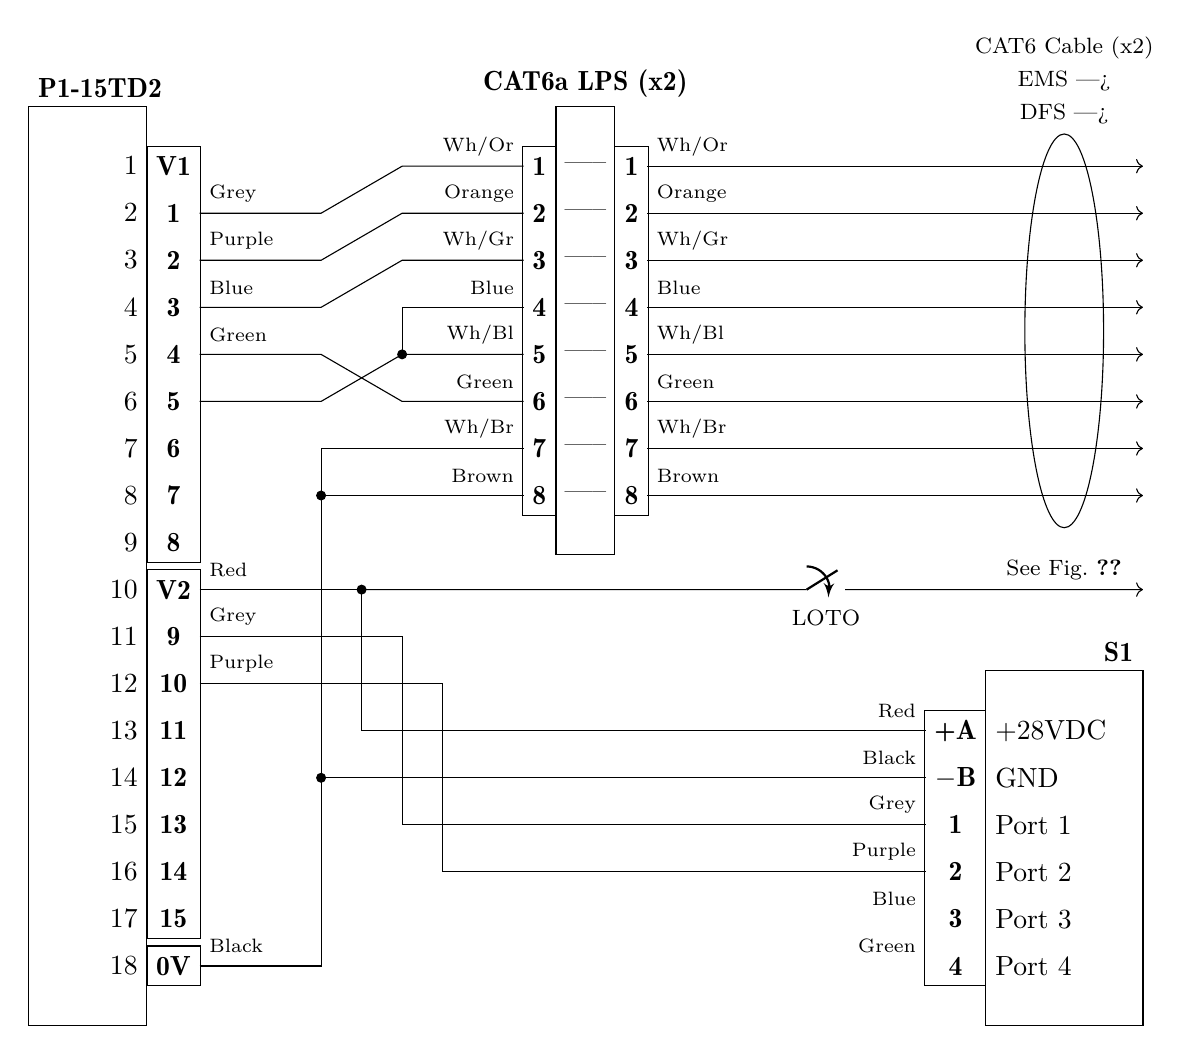
\begin{tikzpicture}
      % \draw[help lines, dashed] grid (12, 3);
      % \draw[help lines, dashed] grid (12, -7);
      % PLC
      \matrix[wire board, wiresright] (plc) {
        1   &  V1  &   \scriptsize \\
        2   &  1   &   \scriptsize Grey \\
        3   &  2   &   \scriptsize Purple \\
        4   &  3   &   \scriptsize Blue \\
        5   &  4   &   \scriptsize Green \\
        6   &  5   &   \scriptsize \\
        7   &  6   &   \scriptsize \\
        8   &  7   &   \scriptsize \\
        9   &  8   &   \scriptsize \\
        10  &  V2  &   \scriptsize Red \\
        11  &  9   &   \scriptsize Grey \\
        12  &  10  &   \scriptsize Purple \\
        13  &  11  &   \scriptsize \\
        14  &  12  &   \scriptsize \\
        15  &  13  &   \scriptsize \\
        16  &  14  &   \scriptsize \\
        17  &  15  &   \scriptsize \\
        18  &  0V  &   \scriptsize Black \\
        };
        \draw (plc-1-2.north east) rectangle (plc-9-1.south east);
        \draw (plc-10-2.north east) rectangle (plc-17-1.south east);
        \draw (plc-18-2.north east) rectangle (plc-18-1.south east);
        \draw (plc-1-2.north west)+(-1.5cm,0.5cm) coordinate(p1) rectangle ($(plc-18-2.south west)+(0,-0.5cm)$);
        \draw (p1) node[anchor=south west, align=left]{\textbf{P1-15TD2}};

        % CAT6 LIGHTNING PROTECTION SYSTEM
        \matrix[wire board, wiresboth, matrix anchor=north, right=5cm of plc.north] (lps) {
          \scriptsize Wh/Or &   1   &  -----  &  1  & \scriptsize Wh/Or\\
          \scriptsize Orange&   2   &  -----  &  2  & \scriptsize Orange\\
          \scriptsize Wh/Gr &   3   &  -----  &  3  & \scriptsize Wh/Gr\\
          \scriptsize Blue  &   4   &  -----  &  4  & \scriptsize Blue\\
          \scriptsize Wh/Bl &   5   &  -----  &  5  & \scriptsize Wh/Bl\\
          \scriptsize Green &   6   &  -----  &  6  & \scriptsize Green\\
          \scriptsize Wh/Br &   7   &  -----  &  7  & \scriptsize Wh/Br\\
          \scriptsize Brown &   8   &  -----  &  8  & \scriptsize Brown\\
        };
        % Boxing the contents
        \draw (lps-1-2.north east) rectangle (lps-8-2.south west);
        \draw (lps-1-4.north east) rectangle (lps-8-4.south west);
        \draw (lps-1-2.north east)+(0cm,0.5cm) rectangle ($(lps-8-4.south west)+(0cm,-0.5cm)$);
        \draw (p1) (current subpath start -| lps-1-3) node[anchor=south, font=\bfseries]{CAT6a LPS (x2)};

        % RF SWITCHES 1
        \path (plc.south) -- ++ (10cm, 0)
        node[matrix, wire board, wiresleft, matrix anchor=south] (shackswitch) {
          \scriptsize Red   &   +A  & +28VDC \\
          \scriptsize Black & $-$B  & GND \\
          \scriptsize Grey  &   1   & Port 1 \\
          \scriptsize Purple&   2   & Port 2 \\
          \scriptsize Blue  &   3   & Port 3 \\
          \scriptsize Green &   4   & Port 4 \\
        };
        \draw (shackswitch-1-2.north west) rectangle (shackswitch-6-3.south west);
        \draw (shackswitch-1-3.north west)+(2cm,0.5cm) coordinate(p3) rectangle ($(shackswitch-6-3.south west)+(0,-0.5cm)$);
        \draw (p3) node[anchor=south east, align=right]{\textbf{S1}};

        % WIRING 
        % plc to lps
        \path(plc-1-3.south west) -- (lps-1-1.south east)
        coordinate[pos=0.25](1q)
        coordinate[pos=0.375](3e)
        coordinate[pos=0.5](m)
        coordinate[pos=0.625](5e)
        coordinate[pos=0.75](3q);
        \draw(plc-2-3.south west) -- (plc-2-1 -| 3e) -- (lps-1-2 -| 5e) -- (lps-1-1.south east);
        \draw(plc-3-3.south west) -- (plc-3-1 -| 3e) -- (lps-2-2 -| 5e) -- (lps-2-1.south east);
        \draw(plc-4-3.south west) -- (plc-4-1 -| 3e) -- (lps-3-2 -| 5e) -- (lps-3-1.south east);
        \draw(plc-5-3.south west) -- (plc-5-1 -| 3e) -- (lps-6-2 -| 5e) -- (lps-6-1.south east);
        \draw(plc-6-3.south west) -- (plc-6-1 -| 3e) -- (lps-5-2 -| 5e) node[circ](asdf){} -- (lps-5-1.south east);
        \draw(asdf) -- (lps-4-2 -| 5e) -- (lps-4-1.south east);
        % plc to shack switch
        \draw(plc-10-3.south west) -- (plc-10-3.south west -| m) node[circ](v2circ){} -- (shackswitch-1-1.south east -| m) -- (shackswitch-1-1.south east);
        \draw(plc-11-3.south west) -- (plc-11-3.south west -| 5e) -- (shackswitch-3-1.south east -| 5e) -- (shackswitch-3-1.south east);
        \draw(plc-12-3.south west) -- (plc-12-3.south west -| 3q) -- (shackswitch-4-1.south east -| 3q) -- (shackswitch-4-1.south east);
        % plc ground wires
        \draw(plc-18-3.south west) -- (plc-18-3.south west -| 3e) -- (shackswitch-2-1.south east -| 3e) node[circ=1pt](gndnode1){};
        \draw(gndnode1) -- (shackswitch-2-1.south east);
        \draw(gndnode1) -- (lps-8-1.south east -| gndnode1) node[circ=1pt](gndnode2){} -- (lps-8-1.south east);
        \draw(gndnode2) |- (lps-7-1.south east);
        % lps cont
        \draw(lps-1-5.south west)[->] -- (lps-1-4 -| p3);
        \draw(lps-2-5.south west)[->] -- (lps-2-4 -| p3);
        \draw(lps-3-5.south west)[->] -- (lps-3-4 -| p3);
        \draw(lps-4-5.south west)[->] -- (lps-4-4 -| p3);
        \draw(lps-5-5.south west)[->] -- (lps-5-4 -| p3);
        \draw(lps-6-5.south west)[->] -- (lps-6-4 -| p3);
        \draw(lps-7-5.south west)[->] -- (lps-7-4 -| p3);
        \draw(lps-8-5.south west)[->] -- (lps-8-4 -| p3);
        % ellipse
        \path(lps-4-3) -- (lps-5-3) coordinate[pos=0.5](lps2midway);
        \draw(lps2midway -| p3)+(-1, 0) ellipse(0.5 and 2.5) coordinate(ellipse);
        \draw(ellipse)+(0, 2.5) node[anchor=south, align=center]{\footnotesize CAT6 Cable (x2)\\\footnotesize EMS --->\\\footnotesize DFS --->};
        % plc to loto
        \draw(v2circ)[->] -- (v2circ -| lps.east) to[switch, name=loto] ++ (2, 0) -- (v2circ -| p3);
        \draw(loto.south) node[anchor=north]{\footnotesize LOTO};
        \draw(v2circ -| ellipse) node[anchor=south]{\footnotesize See Fig.~\ref{fig:serialwiring}};
\end{tikzpicture}
\end{center}
\caption{RFI Shack PLC Line Wiring Diagram.}\label{fig:shackwiring}
\end{figure}

\begin{figure}
  \begin{center}
    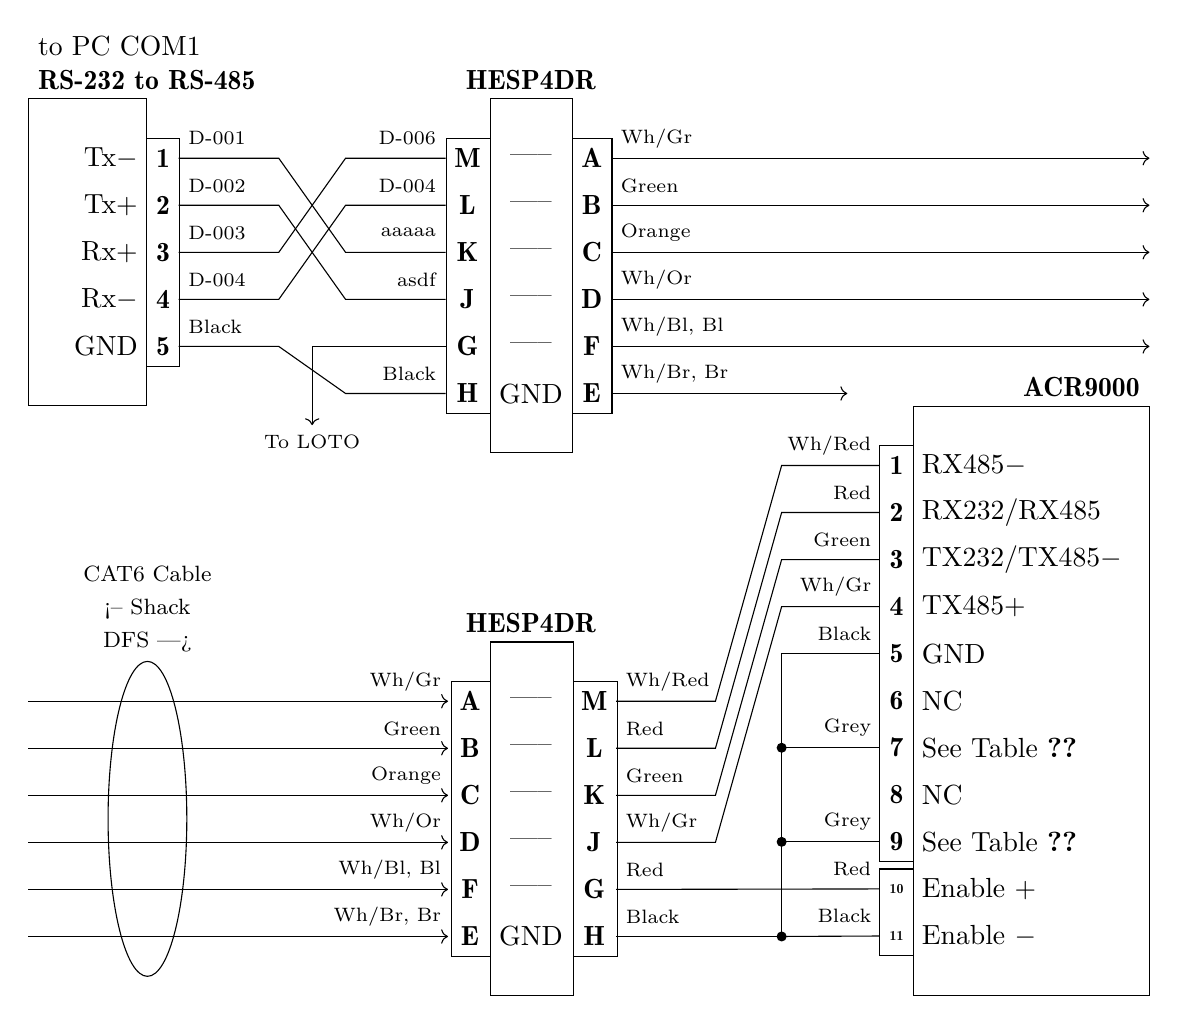
\begin{tikzpicture}
      % \draw[help lines, dashed] grid (12, 3);
      % \draw[help lines, dashed] grid (12, -7);
      % CONVERTER
      \matrix[wire board, wiresright] (converter) {
        Tx$-$ &  1   &   \scriptsize D-001   \\
        Tx+   &  2   &   \scriptsize D-002   \\
        Rx+   &  3   &   \scriptsize D-003   \\
        Rx$-$ &  4   &   \scriptsize D-004   \\
        GND   &  5   &   \scriptsize Black   \\
        };
        \draw (converter-1-2.north east) rectangle (converter-5-2.south west);
        \draw (converter-1-2.north west)+(-1.5cm,0.5cm) coordinate(p1) rectangle ($(converter-5-2.south west)+(0,-0.5cm)$);
        \draw (p1) node[anchor=south west, align=left]{to PC COM1\\\textbf{RS-232 to RS-485}};

        % LIGHTNING PROTECTION SYSTEM
        \matrix[wire board, wiresboth, matrix anchor=north, right=5cm of converter.north] (lps) {
          \scriptsize D-006 &   M   &  -----  &  A  & \scriptsize Wh/Gr\\
          \scriptsize D-004 &   L   &  -----  &  B  & \scriptsize Green\\
          \scriptsize aaaaa &   K   &  -----  &  C  & \scriptsize Orange\\
          \scriptsize asdf  &   J   &  -----  &  D  & \scriptsize Wh/Or\\
          \scriptsize       &   G   &  -----  &  F  & \scriptsize Wh/Bl, Bl\\
          \scriptsize Black &   H   &  GND    &  E  & \scriptsize Wh/Br, Br\\
        };
        % Boxing the contents
        \draw (lps-1-2.north east) rectangle (lps-6-2.south west);
        \draw (lps-1-4.north east) rectangle (lps-6-4.south west);
        \draw (lps-1-2.north east)+(0cm,0.5cm) rectangle ($(lps-6-4.south west)+(0cm,-0.5cm)$);
        \draw (p1) (current subpath start -| lps-1-3) node[anchor=south, font=\bfseries]{HESP4DR};
        % LIGHTNING PROTECTION SYSTEM 2
        \matrix[wire board, wiresboth, matrix anchor=lps2-1-3.north, anchor=north, below=4cm of lps-5-3.south] (lps2) {
          \scriptsize Wh/Gr  &   A   &  -----  &  M  & \scriptsize Wh/Red\\
          \scriptsize Green  &   B   &  -----  &  L  & \scriptsize Red\\
          \scriptsize Orange &   C   &  -----  &  K  & \scriptsize Green\\
          \scriptsize Wh/Or  &   D   &  -----  &  J  & \scriptsize Wh/Gr\\
          \scriptsize Wh/Bl, Bl& F   &  -----  &  G  & \scriptsize Red\\
          \scriptsize Wh/Br, Br& E   &  GND    &  H  & \scriptsize Black\\
        };
        % Boxing the contents
        \draw (lps2-1-2.north east) rectangle (lps2-6-2.south west);
        \draw (lps2-1-4.north east) rectangle (lps2-6-4.south west);
        \draw (lps2-1-2.north east)+(0cm,0.5cm) rectangle ($(lps2-6-4.south west)+(0cm,-0.5cm)$);
        \draw (lps2-1-3.north)+(0, 0.5) node[anchor=south, font=\bfseries]{HESP4DR};

        % DB9 CONNECTOR
        \matrix[wire board, wiresleft, matrix anchor=south, right=5.5cm of lps2.south] (db9) {
          \scriptsize Wh/Red &   1   &   RX485$-$ \\
          \scriptsize Red   &   2   &   RX232/RX485 \\
          \scriptsize Green &   3   &   TX232/TX485$-$ \\
          \scriptsize Wh/Gr &   4   &   TX485+ \\
          \scriptsize Black &   5   &   GND  \\
          \scriptsize       &   6   &   NC \\
          \scriptsize Grey  &   7   &   See Table~\ref{tab:acr9000com1} \\
          \scriptsize       &   8   &   NC \\
          \scriptsize Grey  &   9   &   See Table~\ref{tab:acr9000com1} \\
          \scriptsize Red   &   \tiny10   &   Enable + \\
          \scriptsize Black &   \tiny11   &   Enable $-$ \\
        };
        \draw (db9-1-2.north east) rectangle (db9-9-2.south west);
        \draw (db9-10-2.north east) rectangle (db9-11-2.south west);
        \draw (db9-1-2.north east)+(3cm,0.5cm) coordinate(p3) rectangle ($(db9-11-2.south east)+(0,-0.5cm)$);
        \draw (p3) node[anchor=south east, align=right]{\textbf{ACR9000}};

        % WIRING this is the most hellish thing i've ever done never make a wiring diagram in tikz it isnt worth it
        \path(converter-1-3.south west) -- (lps-1-1.south east)
        coordinate[pos=0.25](1quarter)
        coordinate[pos=0.375](3eighth)
        coordinate[pos=0.5](m)
        coordinate[pos=0.625](5eighth)
        coordinate[pos=0.75](3quarter);
        
        \draw(converter-1-3.south west) -- (3eighth) -- (lps-3-2 -| 5eighth) -- (lps-3-1.south east);
        \draw(converter-2-3.south west) -- (converter-2-2 -| 3eighth) -- (lps-4-2 -| 5eighth) -- (lps-4-1.south east);
        \draw(converter-3-3.south west) -- (converter-3-2 -| 3eighth) -- (5eighth) -- (lps-1-1.south east);
        \draw(converter-4-3.south west) -- (converter-4-2 -| 3eighth) -- (lps-2-2 -| 5eighth) -- (lps-2-1.south east);
        \draw(converter-5-3.south west) -- (converter-5-2 -| 3eighth) -- (lps-6-2 -| 5eighth) -- (lps-6-1.south east);
        \draw(lps-5-1.south east)[->] -- (lps-5-2 -| m) -- ++ (0, -1) node[anchor=north]{\scriptsize To LOTO};

        \path(lps2-1-5.south west) -- (db9-4-1.south east)
        coordinate[pos=0.25](1quarter)
        coordinate[pos=0.375](3eighth)
        coordinate[pos=0.5](m)
        coordinate[pos=0.625](5eighth)
        coordinate[pos=0.75](3quarter);

        \draw(lps-1-5.south west)[->] -- (lps-1-4 -| p3);
        \draw(lps-2-5.south west)[->] -- (lps-2-4 -| p3);
        \draw(lps-3-5.south west)[->] -- (lps-3-4 -| p3);
        \draw(lps-4-5.south west)[->] -- (lps-4-4 -| p3);
        \draw(lps-5-5.south west)[->] -- (lps-5-4 -| p3);
        \draw(lps-6-5.south west)[->] -- ++ (3, 0);

        \draw([xshift=-1pt]lps2-1-1.south east)[<-] -- (lps2-1-2 -| p1);
        \draw([xshift=-1pt]lps2-2-1.south east)[<-] -- (lps2-2-2 -| p1);
        \draw([xshift=-1pt]lps2-3-1.south east)[<-] -- (lps2-3-2 -| p1);
        \draw([xshift=-1pt]lps2-4-1.south east)[<-] -- (lps2-4-2 -| p1);
        \draw([xshift=-1pt]lps2-5-1.south east)[<-] -- (lps2-5-2 -| p1);
        \draw([xshift=-1pt]lps2-6-1.south east)[<-] -- (lps2-6-2 -| p1);

        \path(lps2-3-3) -- (lps2-4-3) coordinate[pos=0.5](lps2midway);
        \draw(lps2midway -| converter-1-1.east) ellipse(0.5 and 2) coordinate(ellipse);
        \draw(ellipse |- lps2-1-3)+(0, 0.5) node[anchor=south, align=center]{\footnotesize CAT6 Cable\\\footnotesize <-- Shack\\\footnotesize DFS --->};
        
        \draw(lps2-1-5.south west) -- (lps2-1-4 -| 3eighth) -- (db9-1-2 -| 5eighth) -- (db9-1-2);
        \draw(lps2-2-5.south west) -- (lps2-2-4 -| 3eighth) -- (db9-2-2 -| 5eighth) -- (db9-2-2);
        \draw(lps2-3-5.south west) -- (lps2-3-4 -| 3eighth) -- (db9-3-2 -| 5eighth) -- (db9-3-2);
        \draw(lps2-4-5.south west) -- (lps2-4-4 -| 3eighth) -- (db9-4-2 -| 5eighth) -- (db9-4-2);
        \draw(lps2-5-5.south west) -- (db9-10-2);
        \draw(lps2-6-5.south west) -- (lps2-6-4 -| 5eighth) node[circ=1pt](gndm){};
        \draw(gndm) -- (db9-11-2);
        \draw(gndm) -- (db9-7-2 -| gndm) node[circ=1pt](gndm2){} -- (db9-7-2);
        \draw(gndm2) |- (db9-5-2);
        \draw(db9-9-2) -- (db9-9-2 -| gndm) node[circ]{};
\end{tikzpicture}
\end{center}
\caption{Shack to DFS Serial and LOTO Line Wiring Diagram.}\label{fig:serialwiring}
\end{figure}
\begin{figure}
  \begin{center}
    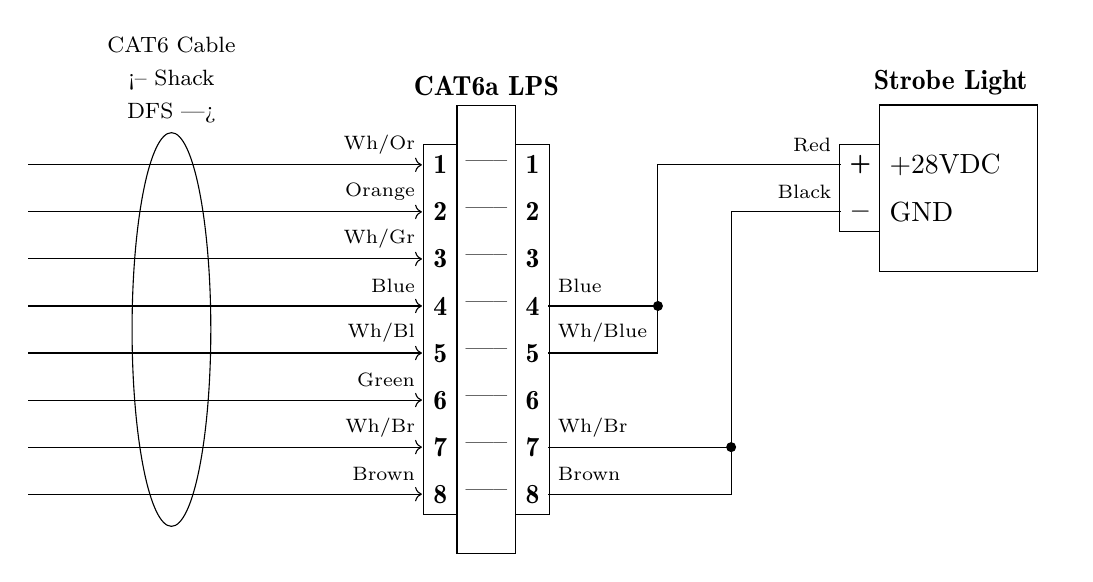
\begin{tikzpicture}
      % \draw[help lines, dashed] grid (12, 3);
      % \draw[help lines, dashed] grid (12, -7);
      % CAT6 LIGHTNING PROTECTION SYSTEM
      \matrix[wire board, wiresboth, matrix anchor=north] (lps) {
        \scriptsize Wh/Or &   1   &  -----  &  1  & \scriptsize \\
        \scriptsize Orange&   2   &  -----  &  2  & \scriptsize \\
        \scriptsize Wh/Gr &   3   &  -----  &  3  & \scriptsize \\
        \scriptsize Blue  &   4   &  -----  &  4  & \scriptsize Blue\\
        \scriptsize Wh/Bl &   5   &  -----  &  5  & \scriptsize Wh/Blue\\
        \scriptsize Green &   6   &  -----  &  6  & \scriptsize \\
        \scriptsize Wh/Br &   7   &  -----  &  7  & \scriptsize Wh/Br\\
        \scriptsize Brown &   8   &  -----  &  8  & \scriptsize Brown\\
      };
      % Boxing the contents
      \draw (lps-1-2.north east) rectangle (lps-8-2.south west);
      \draw (lps-1-4.north east) rectangle (lps-8-4.south west);
      \draw (lps-1-2.north east)+(0cm,0.5cm) rectangle ($(lps-8-4.south west)+(0cm,-0.5cm)$);
      \draw (lps-1-3.north)+(0, 0.5) node[anchor=south, font=\bfseries]{CAT6a LPS};

      % SAFETY LIGHT
      \matrix[wire board, wiresleft, matrix anchor=north, right=5cm of lps.north] (strobe) {
        \scriptsize Red   &   +  & +28VDC \\
        \scriptsize Black &  $-$ & GND \\
      };
      \draw (strobe-1-2.north west) rectangle (strobe-2-3.south west);
      \draw (strobe-1-3.north west)+(2cm,0.5cm) coordinate(p3) rectangle ($(strobe-2-3.south west)+(0,-0.5cm)$);
      \draw (p3) node[anchor=south east, align=right]{\textbf{Strobe Light}};

      % WIRING 
      % to lps
      \draw([xshift=-1pt]lps-1-1.south east)[<-] -- ++ (-5, 0);
      \draw([xshift=-1pt]lps-2-1.south east)[<-] -- ++ (-5, 0);
      \draw([xshift=-1pt]lps-3-1.south east)[<-] -- ++ (-5, 0);
      \draw([xshift=-1pt]lps-4-1.south east)[<-] -- ++ (-5, 0);
      \draw([xshift=-1pt]lps-5-1.south east)[<-] -- ++ (-5, 0);
      \draw([xshift=-1pt]lps-6-1.south east)[<-] -- ++ (-5, 0);
      \draw([xshift=-1pt]lps-7-1.south east)[<-] -- ++ (-5, 0);
      \draw([xshift=-1pt]lps-8-1.south east)[<-] -- ++ (-5, 0);
      % lps to ems switches
      \path(lps-1-5.south west) -- (strobe-1-1.south east)
      coordinate[pos=0.25](1q)
      coordinate[pos=0.375](3e)
      coordinate[pos=0.5](m)
      coordinate[pos=0.625](5e)
      coordinate[pos=0.75](3q);
      \draw(lps-5-5.south west) -- (lps-5-5.south west -| 3e) -- (strobe-1-1.south east -| 3e) -- (strobe-1-1.south east);
      \draw(lps-4-5.south west) -- (lps-4-5.south west -| 3e) node[circ=1pt]{};
      \draw(lps-8-5.south west) -- (lps-8-5.south west -| 5e) -- (strobe-2-1.south east -| 5e) -- (strobe-2-1.south east);
      \draw(lps-7-5.south west) -- (lps-7-5.south west -| 5e) node[circ=1pt]{};
      % ellipse
      \path(lps-4-3) -- (lps-5-3) coordinate[pos=0.5](lps2midway);
      \draw(lps2midway)+(-4, 0) ellipse(0.5 and 2.5) coordinate(ellipse);
      \draw(ellipse)+(0, 2.5) node[anchor=south, align=center]{\footnotesize CAT6 Cable\\\footnotesize <-- Shack\\\footnotesize DFS --->};
      % shift the picture left a bit so it lines up with the figure before
      \path(p3) -- ++ (0.35, 0);
\end{tikzpicture}
\end{center}
\caption{RF-DFS PLC Line Wiring Diagram.}\label{fig:dfscat5wiring}
\end{figure}

\subsection{RF-DFS Components}\label{sec:higdfs}
% motor controller, motors, serial lps
The major components located at the RF-DFS are as follows:
\begin{enumerate}
  \item One Parker Hannifin ACR9000 Motor Controller
  \item Two Parker Hannifin Aries AR-04AE Motor Drivers
  \item One DIN-mounted Sola SDN 2.5-24-100P 24V 2.5A linear power supply
  \item One DIN-mounted Advantech BB-HESP4DR RS-422/485 dataline surge suppressor
  \item One L-com AL-CAT6AJW CAT6a lightning protector
  \item One Global Industrial 12-110VDC forklift strobe light
  \item Two PMA3-14LN+ low noise amplifiers
  \item One 1.7ft lightning rod
\end{enumerate}
Most of these components are located at the base of the pedestal, with the exception of the forklift strobe light which is mounted at the breaker panel inside the DFS fence. All serial, control, and RF lines are run from the shack to a horizontal conduit box at the base of the pedestal. From here, it splits with one conduit line going into the pedestal and another going to the breaker panel.

There are three cables coming from the shack as shown in Figure~\ref{fig:shackblock} -- one coaxial cable and two CAT6 lines. One CAT6 line carries the RS-485 motor control signal and drive enable signal, the other is wired directly to the PLC for controlling the strobe light and reserved for RF-switching upgrades. Refer to Figures~\ref{fig:serialwiring} and~\ref{fig:dfscat5wiring} to ensure correct wiring of these components.

Inside the pedestal, the ACR9000 and Aries drives are connected as referenced in the \textit{ACR9000 Hardware Installation Guide}. The ACR9000's 5-24 volt \textit{Drive Enable} signal is connected to the lockout-tagout switch in the shack.

The feed and LNA housing are mounted at the apex of the dish with four all-thread rods in a square pattern. The lightning rod is mounted above this using the same all-thread.

\subsection{RF-EMS Components}\label{sec:higems}
% switching, amplifiers, lps,
The major components located on the RF-EMS tower are as follows:
\begin{enumerate}
  \item One Electro-Metrics EM-6857 omnidirectional club antenna
  \item Three lightning rods
  \item Panel containing:
  \begin{enumerate}
    \item One IEC 60320 C14 AC power receptacle
    \item One AC line filter
    \item One L-com AL-CAT6AJW CAT6a lightning protectors
    \item One Standard Power SPS 15-5 5V 1.5A linear power supply
    \item One Condor HB12-1.7-A+ 12V 1.7A linear power supply
    \item One Condor HBB15-1.5-A+ 15V 1.5A linear power supply
    \item One Condor HB28-1-A+ 28V 1A linear power supply
    \item Two Dynatech Microwave M4-413K201L SP4T relay switches
    \item Two PMA3-14LN+ low noise amplifiers
  \end{enumerate}
\end{enumerate}
The panel components are connected to eachother through a terminal block similar to the one seen in the RFI shack. The 4 power supplies provide DC power to all of the RF components although only the 12 and 28 volt supplies are used for the LNAs and switches, respectively. The other two power supplies remain from previous iterations of this system and can be used for future upgrades. This terminal block also connects the CAT6 LPS and its lines from the shack to RF switches S2 and S3 as shown in Figure~\ref{fig:emscat5wiring}
\begin{figure}[ht]
  \begin{center}
    \begin{circuitikz}
      % AC power
      \draw(0, 0) node[ocirc](ac){};
      \draw(ac.west) node[anchor=east]{120 VAC};
      \draw(ac) -- ++ (1, 0)
      node[lowpass2shape, anchor=west](lpf){};
      % Circle nodes
      \draw(lpf.east) -- ++ (2, 0)
      node[circ](c1){} -- ++ (2, 0)
      node[circ](c2){} -- ++ (2, 0)
      node[circ](c3){} -- ++ (2, 0)
      node[circ](c4){};
      \draw(c1) -- ++ (0, -0.5) node[sacdcshape, anchor=north](dc1){};
      \draw(c2) -- ++ (0, -0.5) node[sacdcshape, anchor=north](dc2){};
      \draw(c3) -- ++ (0, -0.5) node[sacdcshape, anchor=north](dc3){};
      \draw(c4) -- ++ (0, -0.5) node[sacdcshape, anchor=north](dc4){};
      % AC/DC power supplies
      \draw(dc1.south) node[anchor=north west, color=brown]{\footnotesize 5VDC};
      \draw(dc2.south) node[anchor=north west, color=orange]{\footnotesize 12VDC};
      \draw(dc3.south) node[anchor=north west, color=yellow!60!orange!100]{\footnotesize 15VDC};
      \draw(dc4.south) node[anchor=north west, color=red]{\footnotesize 28VDC};
      % Terminal block
      \draw(dc1.south west) ++ (-1, -1.5) coordinate(termblocknw);
      \draw(termblocknw -| dc4.south east) coordinate(termblockne); 
      \draw(dc4.south east) ++ (0, -2.5) coordinate(termblockse);
      \draw(termblocknw |- termblockse) coordinate(termblocksw); 
      \draw(termblocknw) rectangle (termblockse);
      \foreach \x in {0,1,...,15} {
        \draw([xshift=0.25cm]termblocknw) ++ (\x*0.5cm, 0) coordinate(here) -- (here |- termblocksw);
        }
        \foreach \x in {0,1,...,14} {
        \path([xshift=0.50cm]termblocknw) ++ (\x*0.5cm, 0) coordinate(here) -- (here |- termblocksw) node[ocirc, midway](term\x){};
      }
      \draw(termblocknw |- term0) node[anchor=east](termlabel){Terminal Block};
      % Wires from power supply to terminal block
      \draw(dc1.south)[thick] -- (dc1.south |- termblocknw);
      \draw(dc2.south)[thick] -- (dc2.south |- termblocknw);
      \draw(dc3.south)[thick] -- (dc3.south |- termblocknw);
      \draw(dc4.south)[thick] -- (dc4.south |- termblocknw);
      \draw(dc1.south)[thick, dashed, brown] -- (dc1.south |- termblocknw);
      \draw(dc2.south)[thick, dashed, orange] -- (dc2.south |- termblocknw);
      \draw(dc3.south)[thick, dashed, yellow!60!orange!100] -- (dc3.south |- termblocknw);
      \draw(dc4.south)[thick, dashed, red] -- (dc4.south |- termblocknw);
      \draw(dc1.south |- termblocknw) node[anchor=south west, color=brown]{\footnotesize Brown};
      \draw(dc2.south |- termblocknw) node[anchor=south west, color=orange, inner ysep = 1.5pt]{\footnotesize Orange};
      \draw(dc3.south |- termblocknw) node[anchor=south west, color=yellow!60!orange!100]{\footnotesize Yellow};
      \draw(dc4.south |- termblocknw) node[anchor=south west, color=red]{\footnotesize Red};
      % LPS
      \path(dc1.south |- termblocknw) -- coordinate[midway](dc1m) (dc1.south);
      \draw(ac |- dc1m)[blue] node[ocirc](cat6){} to[tmultiwire=8] (dc1m -| term0) -- (termblocknw -| term0);
      \draw(cat6.west) node[anchor=east, blue]{CAT6a};
      
    \end{circuitikz}
  \end{center}
  \caption{RF-EMS Power Connection Diagram.}\label{fig:emsblock}
\end{figure}

\begin{figure}
  \begin{center}
    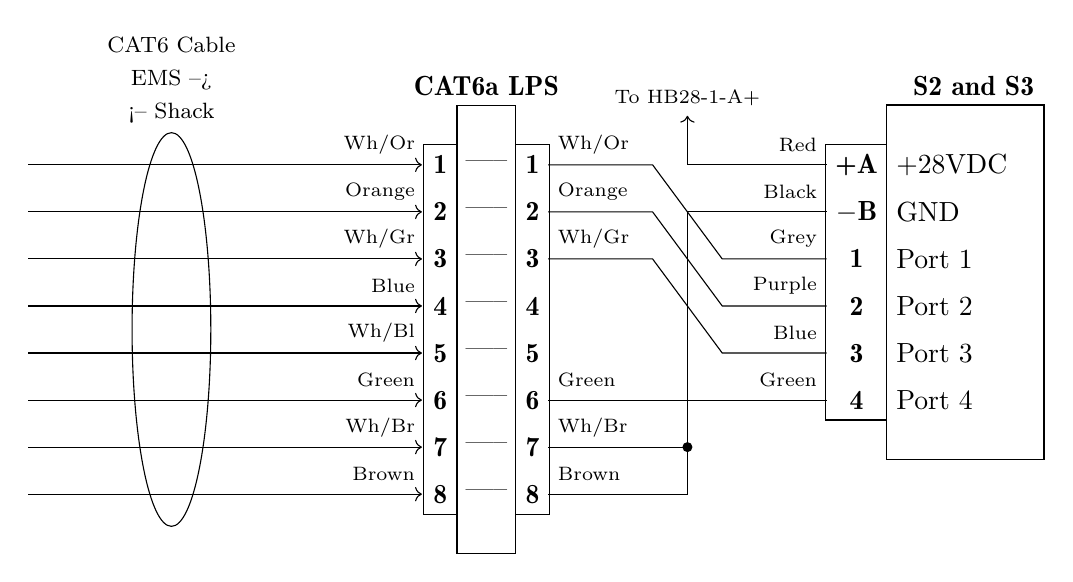
\begin{tikzpicture}
      % \draw[help lines, dashed] grid (12, 3);
      % \draw[help lines, dashed] grid (12, -7);
      % CAT6 LIGHTNING PROTECTION SYSTEM
      \matrix[wire board, wiresboth, matrix anchor=north] (lps) {
        \scriptsize Wh/Or &   1   &  -----  &  1  & \scriptsize Wh/Or\\
        \scriptsize Orange&   2   &  -----  &  2  & \scriptsize Orange\\
        \scriptsize Wh/Gr &   3   &  -----  &  3  & \scriptsize Wh/Gr\\
        \scriptsize Blue  &   4   &  -----  &  4  & \scriptsize \\
        \scriptsize Wh/Bl &   5   &  -----  &  5  & \scriptsize \\
        \scriptsize Green &   6   &  -----  &  6  & \scriptsize Green\\
        \scriptsize Wh/Br &   7   &  -----  &  7  & \scriptsize Wh/Br\\
        \scriptsize Brown &   8   &  -----  &  8  & \scriptsize Brown\\
      };
      % Boxing the contents
      \draw (lps-1-2.north east) rectangle (lps-8-2.south west);
      \draw (lps-1-4.north east) rectangle (lps-8-4.south west);
      \draw (lps-1-2.north east)+(0cm,0.5cm) rectangle ($(lps-8-4.south west)+(0cm,-0.5cm)$);
      \draw (lps-1-3.north)+(0, 0.5) node[anchor=south, font=\bfseries]{CAT6a LPS};

      % RF SWITCHES 2 AND 3
      \matrix[wire board, wiresleft, matrix anchor=north, right=5cm of lps.north] (emsswitches) {
        \scriptsize Red   &   +A  & +28VDC \\
        \scriptsize Black & $-$B  & GND \\
        \scriptsize Grey  &   1   & Port 1 \\
        \scriptsize Purple&   2   & Port 2 \\
        \scriptsize Blue  &   3   & Port 3 \\
        \scriptsize Green &   4   & Port 4 \\
      };
      \draw (emsswitches-1-2.north west) rectangle (emsswitches-6-3.south west);
      \draw (emsswitches-1-3.north west)+(2cm,0.5cm) coordinate(p3) rectangle ($(emsswitches-6-3.south west)+(0,-0.5cm)$);
      \draw (p3) node[anchor=south east, align=right]{\textbf{S2 and S3}};

      % WIRING 
      % to lps
      \draw([xshift=-1pt]lps-1-1.south east)[<-] -- ++ (-5, 0);
      \draw([xshift=-1pt]lps-2-1.south east)[<-] -- ++ (-5, 0);
      \draw([xshift=-1pt]lps-3-1.south east)[<-] -- ++ (-5, 0);
      \draw([xshift=-1pt]lps-4-1.south east)[<-] -- ++ (-5, 0);
      \draw([xshift=-1pt]lps-5-1.south east)[<-] -- ++ (-5, 0);
      \draw([xshift=-1pt]lps-6-1.south east)[<-] -- ++ (-5, 0);
      \draw([xshift=-1pt]lps-7-1.south east)[<-] -- ++ (-5, 0);
      \draw([xshift=-1pt]lps-8-1.south east)[<-] -- ++ (-5, 0);
      % lps to ems switches
      \path(lps-1-5.south west) -- (emsswitches-1-1.south east)
      coordinate[pos=0.25](1q)
      coordinate[pos=0.375](3e)
      coordinate[pos=0.5](m)
      coordinate[pos=0.625](5e)
      coordinate[pos=0.75](3q);
      \draw(lps-1-5.south west) -- (lps-1-5.south west -| 3e) -- (emsswitches-3-2 -| 5e) -- (emsswitches-3-1.south east);
      \draw(lps-2-5.south west) -- (lps-2-5.south west -| 3e) -- (emsswitches-4-2 -| 5e) -- (emsswitches-4-1.south east);
      \draw(lps-3-5.south west) -- (lps-3-5.south west -| 3e) -- (emsswitches-5-2 -| 5e) -- (emsswitches-5-1.south east);
      \draw(lps-6-5.south west) -- (emsswitches-6-1.south east);
      \draw(lps-8-5.south west) -- (lps-8-5.south west -| m) -- (emsswitches-2-1.south east -| m) -- (emsswitches-2-1.south east);
      \draw(lps-7-5.south west) -- (lps-7-5.south west -| m) node[circ=1pt]{};
      \draw(emsswitches-1-1.south east)[->] -- (m) -- (m |- emsswitches.north) node[anchor=south]{\scriptsize To HB28-1-A+};
      % ellipse
      \path(lps-4-3) -- (lps-5-3) coordinate[pos=0.5](lps2midway);
      \draw(lps2midway)+(-4, 0) ellipse(0.5 and 2.5) coordinate(ellipse);
      \draw(ellipse)+(0, 2.5) node[anchor=south, align=center]{\footnotesize CAT6 Cable\\\footnotesize EMS -->\\\footnotesize <-- Shack};
\end{tikzpicture}
\end{center}
\caption{RF-EMS PLC Line Wiring Diagram.}\label{fig:emscat5wiring}
\end{figure}

\section{Communications}\label{sec:comms}
% maybe put pinouts and connections here instead to keep them all together
The Python program controls communications with all off the necessary instruments but it is still necessary for a user to understand how these communications are facilitated in order to troubleshoot issues. The following sections describe how to open communications with each instrument manually and using the Python program.

\subsection{Spectrum Analyzer}\label{sec:commssa}
% scpi commands, how it works, etc, explain not to issue commands while program is running
SCPI commands are issued to the spectrum analyzer via the PyVISA module, this uses an NI-VISA backend and requires it for the program to function. If the user is running the program for the first time, connection should be tested with the NI-VISA Interactive Control program before attempting to use the Python interface. Once a connection is established, issue an identify (\verb|*IDN?|) query to determine that the correct device is connected. Although SCPI commands are relatively universal among instruments, the Python interface is still hard-coded for compatibility with the Keysight N9040B. If a different spectrum analyzer is used, there is no guarantee that it retains the same commands and features as the N9040B, thus some of the issued commands may throw exceptions in the Python interface. 

If the user cannot connect to the spectrum analyzer with NI-VISA, the Python interface will not be able to connect either and they must troubleshoot any errors with hardware connections, drivers, and/or the NI-VISA installation.

Immediately after connecting to an instrument (Described in Section~\ref{sec:usingtheprogram}), the Python interface will attempt to identify the device and display the name above the spectrum plot (See \verb|FrontEnd.initDevice()| in \verb|main.py|). If the connection is successful, the thread running \verb|SpecAn.analyzerDisplayLoop()| in \verb|main.py| will initialize the spectrum plot by issuing \verb|*RST|, querying errors stored on the spectrum analyzer, and querying all values displayed by the widgets to the right of the spectrum plot on the Python interface in Figure~\ref{fig:gui}. If this is successful, The spectrum plot will populate with the same points present on the spectrum analyzer's display and the control panel on the right will populate similarly. Any errors during this process will raise an exception and be output in the terminal.

Care should be taken when issuing SCPI commands either through the terminal, NI-VISA, or the spectrum analyzer's display while the Python program is running in \verb|Continuous| mode as this will likely generate race conditions and raise an exception. When the program is in \verb|Single Sweep| mode, no SCPI commands are issued although the thread running \verb|SpecAn.analyzerDisplayLoop()| will continue to check if a session is open to the device.

\subsection{Motor Controller}\label{sec:commsmc}
% aries command reference stuff here, what bits are used
Communication with the ACR9000 motor controller is facilitated by serial connection over a DB9 cable from the RFI shack. The computer outputs RS-232 which is converted to 4-wire RS-485 before leaving the shack. The ACR9000 also communicates with the Aries azimuth and elevation servo drives via RS-232/485 but this is not controlled, interrupted, or monitored by the PC or Python program in any way.

The language used when sending commands to the ACR9000 is Parker Hannifin's own AcroBASIC, this is a robust language with lots of functionality although at the cost of user-friendliness. The user should reference Parker Hannifin's \textit{ACR Command Language Reference} when troubleshooting problems and making changes to the codebase.

The user can test communication and function at any time using a serial terminal emulator such as PuTTY, TeraTerm, etc., with the default configuration of 9600 baud, 8 data bits, no parity, 1 stop bit, and no flow control. The same precautions for generating race conditions should be taken as in Section~\ref{sec:commssa}. To control the DFS with a terminal emulator, open a connection to the ACR9000 and send a CRLF (Enter), the response from the ACR9000 will show the \textit{Prompt Level} of the device.\ \verb|SYS| is the highest communication level from which the user can navigate to \verb|PROGx| or \verb|PLCx| by typing the aforementioned level and pressing \verb|Enter|, where \verb|x| is a non-negative integer (usually 0).\ \verb|PROG0| is the communication level from which all of the commands used by the Python program will be sent, some relevant commands are listed in Table~\ref{tab:acrcommands}.

\subsubsection{Motor Position}
There is a distinction with how the Python program receives motor position information and how it sends move commands. The ACR9000 initializes its axes to 0 degrees azimuth and 0 degrees elevation when powered on. This causes a problem if the antenna is not parked before being powered down. Because of this, the Python program instead queries encoder position and calculates a vector based on hard-coded encoder positions for x and y axis home in \verb|config.toml| and \verb|defaultconfig.py|. Moving, however, is done by sending \verb|JOG INC| commands in degrees.

The user should regularly calibrate both axes with a level and compass to ensure that the recorded encoder positions for a parked antenna are accurately representative.

\begin{table}[ht]
  \begin{center}\rowcolors{1}{lightgray!30}{white}
    \begin{tabularx}{\linewidth}{p{2cm}|>{\raggedright\arraybackslash}X|>{\raggedright\arraybackslash}X}
      Command          & Function & Example \\ \hline

      \lstinline|PROG| &
      This command switches the communication channel to the designated
      program prompt. &
      The prompt keeps track of your current program or system level as follows: \newline
      \lstinline|SYS>PROG3| \newline
      \lstinline|P03>PROG0| \newline
      \lstinline|P00>SYS| \newline
      \lstinline|SYS>_|
      \\

      \lstinline|DRIVE| \newline
      \lstinline|DRIVE ON| \newline
      \lstinline|DRIVE OFF| \newline
      \lstinline|DRIVE RES|
      &
      The \lstinline|DRIVE| command provides a report-back of the drive's status, lets you
      energize/de-energizes a motor/drive combination or reset the drive. &
      The following example reports the drive status of axis X. \newline
      \lstinline|P00>DRIVE X| \newline
      \lstinline|DRIVE OFF| \newline
      \lstinline|P00>_|
      \\

      \lstinline|JOG| \newline
      \lstinline|JOG ABS| \newline
      \lstinline|JOG INC| &

      Jogging, used along with a second command, sets up an individual velocity profile for an axis to a given velocity, generating a jog offset. This offset can be absolute or incremental from the current position. &
      The following example moves the X axis 5 degrees and Y axis 10 degrees, then back. \newline
      \lstinline|P00>JOG INC X 5| \newline
      \lstinline|P00>JOG INC Y 10| \newline
      \lstinline|P00>JOG ABS X 0 Y 0| \newline
      \lstinline|P00>_|
      \\

      \lstinline|PRINT| \newline
      \lstinline|PRINT BIT792| \newline
      \lstinline|PRINT BIT824| \newline
      \lstinline|PRINT P6144| \newline
      \lstinline|PRINT P6160|
      &
      This command prints a series of expressions (parameter, bit, and string values) to a device. Bits 792 and 824 return -1 if the X and Y axis are moving and 0 if stationary, respectively. Parameters 6144 and 6160 return the X and Y axis encoder positions, respectively. &
      The following example checks if the X axis is moving, then checks its encoder position. \newline
      \lstinline|P00>PRINT BIT792| \newline
      \lstinline|0| \newline
      \lstinline|P00>PRINT P6144| \newline
      \lstinline|-235753513| \newline
      \lstinline|P00>_|
    \end{tabularx}
  \end{center}\rowcolors{1}{white}{white}
  \caption{ACR9000 Commands Used by the Python Program.}\label{tab:acrcommands}
\end{table}

\subsection{PLC}\label{sec:commsplc}
The P1AM-100 uses a SAMD21G18 microcontroller and is programmed with the Arduino Framework, the IDE for this is PlatformIO in VSCode. The P1AM family library should be referenced when making changes to the firmware. Additionally, care should be taken when updating opcodes to also make changes in the Python declaration (See \verb|opcodes.h| and \verb|opcodes.py|).

The basic flow of control in the PLC firmware is to wait for information in the serial buffer, then parse it as it arrives. Opcodes will be expected as a string of binary ASCII characters terminated by a newline character. If the opcode is recognized, the PLC will perform the expected operation and write a response to the serial buffer if necessary.

\section{Software User Guide}
The following section describes how to use the Python interface to connect to and control each instrument. Refer to Figure~\ref{fig:gui} for an image of the root GUI window.

\subsection{Getting Started}
% software installation stuff, ni-visa, other requirements
In order to use the front-end interface, download the following deployment requirements and the latest release on \verb|EMSMONPC2|, then run the executable. Releases are located at the following link: \url{https://github.com/RomiFC/RF-DFS/releases}.
\begin{enumerate}
  \item NI-VISA
  \item NI-488.2 if the spectrum analyzer is connected via GPIB
\end{enumerate}

\subsection{Using the Program}\label{sec:usingtheprogram}
After starting the program, navigate to \verb|Options>Configure| at the top left banner to connect to the appropriate devices/COM ports. The \verb|Connection Status| window will let you know if a device is connected, however, it is up to the user to ensure that the correct device has been selected in the \verb|Configure| menu. The terminal will output any initialization errors (such as if the wrong device/port is selected).

From here, the user can issue SCPI commands to the spectrum analyzer using the control panel on the right, issue motor commands using the \verb|Antenna Position| panel, or select RF chains using the \verb|PLC Operations| panel on the left if it has been initialized. Commands can be issued to the spectrum analyzer by either selecting a button or typing an entry and pressing \verb|Enter|. All entries will be issued in base units for the given parameter (Hz, seconds, etc.), however, shorthand scientific notation is allowed (\verb|5e9| will be passed as 5 GHz).

\begin{figure}
  \begin{center}
    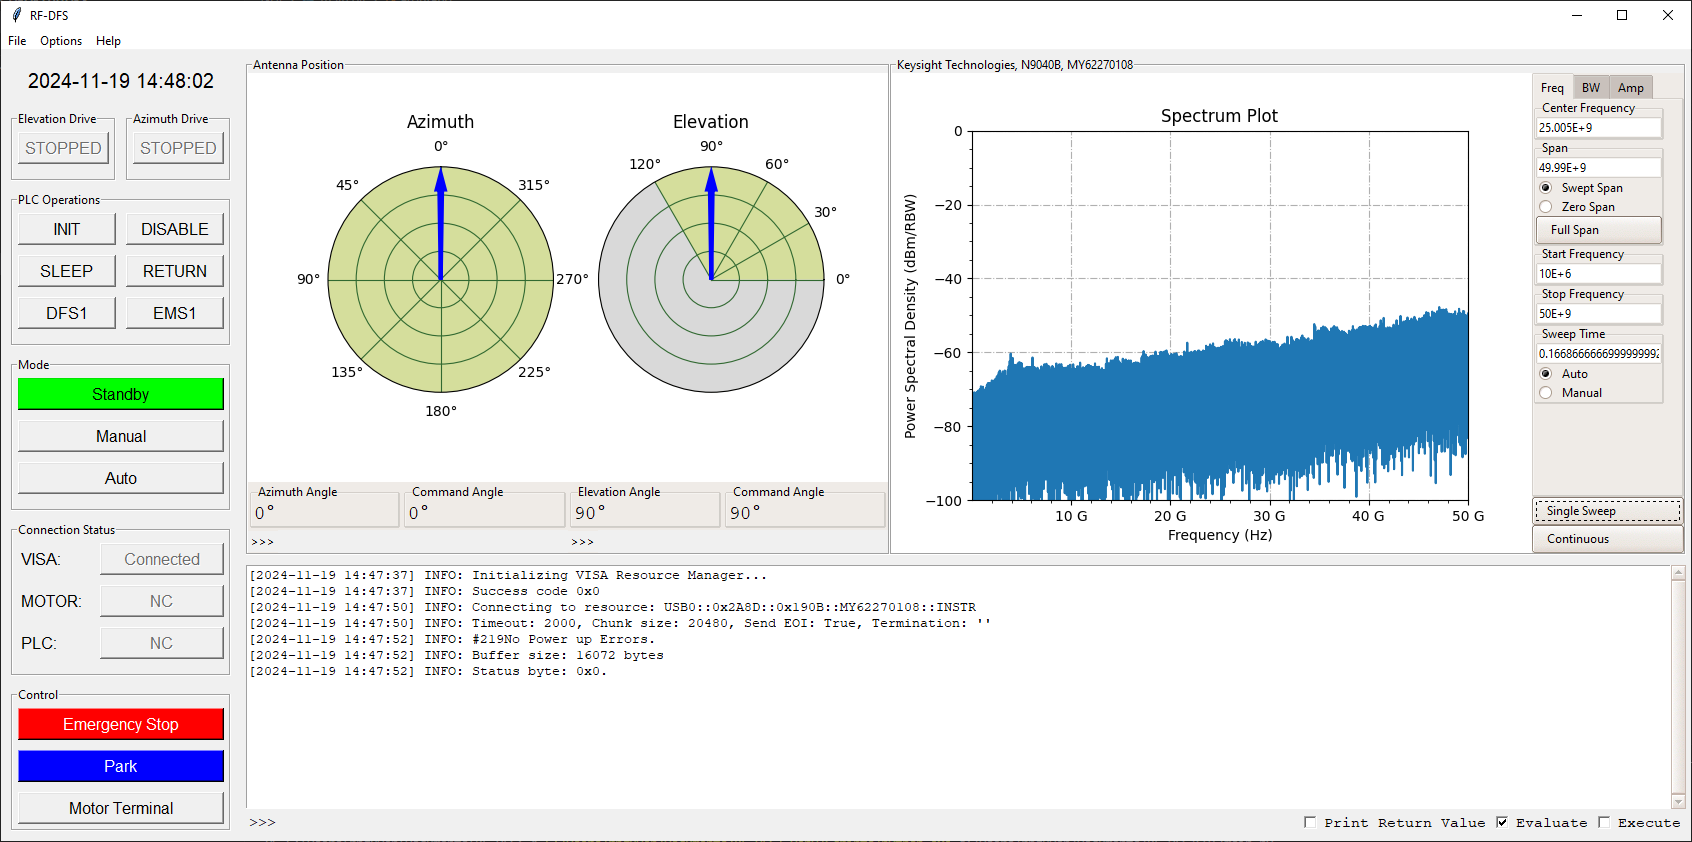
\includegraphics[width=\textwidth]{images/3gui.png}
  \end{center}
  \caption{Python Graphical User Interface.}\label{fig:gui}
\end{figure}

\subsubsection{Terminal}
The terminal at the bottom of the window will be the primary means of communicating information and exceptions to the user. Exceptions are not unconditionally fatal, but they should be noted to investigate if the problem lies in hardware or software. The user should consider saving a log of the terminal under \verb|File>Save log| if necessary. Up and down arrow keys can be used to access previously issued commands to the terminal.

Python commands can also be evaluated or executed in the terminal, the difference between both commands is described in the Python documentation. It is highly recommended to reference the source code when issuing terminal commands, as this has the potential for deadlock, race conditions, and other undefined scenarios if care is not taken. Instances, their attributes, and methods, can all be accessed using the terminal although all commands will be generated in the main thread. As a result, most IO calls will be blocking for the duration of their execution. This can be avoided by using a thread handler, if it exists in the appropriate scope, or generating a thread for the given IO call. See:

\verb|SpecAn.setAnalyzerThreadHandler|:
\begin{lstlisting}[language=Python]
class SpecAn(FrontEnd):
    def setAnalyzerThreadHandler(self, *event, **kwargs):
        _dict = {}
        for key in kwargs:
            _dict[key] = kwargs.get(key)
        thread = threading.Thread(target=self.setAnalyzerValue, kwargs=_dict)
        thread.start()
\end{lstlisting}

\verb|SerialIO.threadHandler|:
\begin{lstlisting}[language=Python]
class SerialIO:
    def threadHandler(self, target, args=(), kwargs={}):
        if not hasattr(SerialIO, target.__name__):
            logging.error(f'Class SerialIO does not contain a method with identifier {target.__name__}')
            return
        thread = threading.Thread(target = target, args = args, kwargs = kwargs, daemon=True)
        thread.start()
\end{lstlisting}

Or, if generating a thread using the \verb|Execute| function, use semicolons to separate lines of code.
\begin{lstlisting}[language=Python]
thread=threading.Thread(target=Vi.openRsrc.write, args=(":SENS:FREQ:STOP 10e9",), daemon=True);thread.start()
\end{lstlisting}
Is equivalent to\dots
\begin{lstlisting}[language=Python]
thread=threading.Thread(target=Vi.openRsrc.write, args=(":SENS:FREQ:STOP 10e9",), daemon=True)
thread.start()
\end{lstlisting}  

\section{Appendix}
\subsection{Development}
Design files are located in the git repository hosted at \url{https://github.com/RomiFC/RF-DFS}. The wiki and \verb|README.md| files contain instructions for setting up a development environment for the Python software and PLC firmware. Functions, methods, and classes, should all be documented with a Python docstring or C/C++ Doxygen brief. Constants and global variables should be declared at the top of each file, below the header and library imports.

Board files are also located in this repository with instructions for importing libraries to the local project directory. Each board contains a changelog located in the \verb|README.md| which contains vital information for distinguishing flaws and fixes between revisions. Each print with a change from the last print should iterate the revision and be documented in the changelog.

\subsection{Receiver Upgrades}
As stated in Section~\ref{sec:rfchain}, this upgrade provides the framework to add additional receivers relatively easily. The Mini-Circuits PMA-183PLN+ was picked as an input stage LNA for a 6--18 GHz receiver although downconverting components would still need to be sourced. Figure~\ref{fig:pma183} shows the measured s-parameters for a designed and assembled amplifier which prove reasonable. Mini-Circuits also claims a nominal 1.4 dB noise figure within the operating frequency which is comparable to the PMA3-14LN+ at a nominal 1.8 dB.

\begin{figure}[!ht]
  \begin{center}
    %% Creator: Matplotlib, PGF backend
%%
%% To include the figure in your LaTeX document, write
%%   \input{<filename>.pgf}
%%
%% Make sure the required packages are loaded in your preamble
%%   \usepackage{pgf}
%%
%% Also ensure that all the required font packages are loaded; for instance,
%% the lmodern package is sometimes necessary when using math font.
%%   \usepackage{lmodern}
%%
%% Figures using additional raster images can only be included by \input if
%% they are in the same directory as the main LaTeX file. For loading figures
%% from other directories you can use the `import` package
%%   \usepackage{import}
%%
%% and then include the figures with
%%   \import{<path to file>}{<filename>.pgf}
%%
%% Matplotlib used the following preamble
%%   \def\mathdefault#1{#1}
%%   \everymath=\expandafter{\the\everymath\displaystyle}
%%   
%%   \ifdefined\pdftexversion\else  % non-pdftex case.
%%     \usepackage{fontspec}
%%   \fi
%%   \makeatletter\@ifpackageloaded{underscore}{}{\usepackage[strings]{underscore}}\makeatother
%%
\begingroup%
\makeatletter%
\begin{pgfpicture}%
\pgfpathrectangle{\pgfpointorigin}{\pgfqpoint{4.416023in}{3.339900in}}%
\pgfusepath{use as bounding box, clip}%
\begin{pgfscope}%
\pgfsetbuttcap%
\pgfsetmiterjoin%
\definecolor{currentfill}{rgb}{1.000000,1.000000,1.000000}%
\pgfsetfillcolor{currentfill}%
\pgfsetlinewidth{0.000000pt}%
\definecolor{currentstroke}{rgb}{1.000000,1.000000,1.000000}%
\pgfsetstrokecolor{currentstroke}%
\pgfsetdash{}{0pt}%
\pgfpathmoveto{\pgfqpoint{0.000000in}{0.000000in}}%
\pgfpathlineto{\pgfqpoint{4.416023in}{0.000000in}}%
\pgfpathlineto{\pgfqpoint{4.416023in}{3.339900in}}%
\pgfpathlineto{\pgfqpoint{0.000000in}{3.339900in}}%
\pgfpathlineto{\pgfqpoint{0.000000in}{0.000000in}}%
\pgfpathclose%
\pgfusepath{fill}%
\end{pgfscope}%
\begin{pgfscope}%
\pgfsetbuttcap%
\pgfsetmiterjoin%
\definecolor{currentfill}{rgb}{1.000000,1.000000,1.000000}%
\pgfsetfillcolor{currentfill}%
\pgfsetlinewidth{0.000000pt}%
\definecolor{currentstroke}{rgb}{0.000000,0.000000,0.000000}%
\pgfsetstrokecolor{currentstroke}%
\pgfsetstrokeopacity{0.000000}%
\pgfsetdash{}{0pt}%
\pgfpathmoveto{\pgfqpoint{0.643596in}{0.515000in}}%
\pgfpathlineto{\pgfqpoint{4.142411in}{0.515000in}}%
\pgfpathlineto{\pgfqpoint{4.142411in}{3.040900in}}%
\pgfpathlineto{\pgfqpoint{0.643596in}{3.040900in}}%
\pgfpathlineto{\pgfqpoint{0.643596in}{0.515000in}}%
\pgfpathclose%
\pgfusepath{fill}%
\end{pgfscope}%
\begin{pgfscope}%
\pgfpathrectangle{\pgfqpoint{0.643596in}{0.515000in}}{\pgfqpoint{3.498815in}{2.525900in}}%
\pgfusepath{clip}%
\pgfsetrectcap%
\pgfsetroundjoin%
\pgfsetlinewidth{0.803000pt}%
\definecolor{currentstroke}{rgb}{0.690196,0.690196,0.690196}%
\pgfsetstrokecolor{currentstroke}%
\pgfsetdash{}{0pt}%
\pgfpathmoveto{\pgfqpoint{0.643596in}{0.515000in}}%
\pgfpathlineto{\pgfqpoint{0.643596in}{3.040900in}}%
\pgfusepath{stroke}%
\end{pgfscope}%
\begin{pgfscope}%
\pgfsetbuttcap%
\pgfsetroundjoin%
\definecolor{currentfill}{rgb}{0.000000,0.000000,0.000000}%
\pgfsetfillcolor{currentfill}%
\pgfsetlinewidth{0.803000pt}%
\definecolor{currentstroke}{rgb}{0.000000,0.000000,0.000000}%
\pgfsetstrokecolor{currentstroke}%
\pgfsetdash{}{0pt}%
\pgfsys@defobject{currentmarker}{\pgfqpoint{0.000000in}{-0.048611in}}{\pgfqpoint{0.000000in}{0.000000in}}{%
\pgfpathmoveto{\pgfqpoint{0.000000in}{0.000000in}}%
\pgfpathlineto{\pgfqpoint{0.000000in}{-0.048611in}}%
\pgfusepath{stroke,fill}%
}%
\begin{pgfscope}%
\pgfsys@transformshift{0.643596in}{0.515000in}%
\pgfsys@useobject{currentmarker}{}%
\end{pgfscope}%
\end{pgfscope}%
\begin{pgfscope}%
\definecolor{textcolor}{rgb}{0.000000,0.000000,0.000000}%
\pgfsetstrokecolor{textcolor}%
\pgfsetfillcolor{textcolor}%
\pgftext[x=0.643596in,y=0.417777in,,top]{\color{textcolor}{\rmfamily\fontsize{10.000000}{12.000000}\selectfont\catcode`\^=\active\def^{\ifmmode\sp\else\^{}\fi}\catcode`\%=\active\def%{\%}$\mathdefault{0}$}}%
\end{pgfscope}%
\begin{pgfscope}%
\pgfpathrectangle{\pgfqpoint{0.643596in}{0.515000in}}{\pgfqpoint{3.498815in}{2.525900in}}%
\pgfusepath{clip}%
\pgfsetrectcap%
\pgfsetroundjoin%
\pgfsetlinewidth{0.803000pt}%
\definecolor{currentstroke}{rgb}{0.690196,0.690196,0.690196}%
\pgfsetstrokecolor{currentstroke}%
\pgfsetdash{}{0pt}%
\pgfpathmoveto{\pgfqpoint{1.080948in}{0.515000in}}%
\pgfpathlineto{\pgfqpoint{1.080948in}{3.040900in}}%
\pgfusepath{stroke}%
\end{pgfscope}%
\begin{pgfscope}%
\pgfsetbuttcap%
\pgfsetroundjoin%
\definecolor{currentfill}{rgb}{0.000000,0.000000,0.000000}%
\pgfsetfillcolor{currentfill}%
\pgfsetlinewidth{0.803000pt}%
\definecolor{currentstroke}{rgb}{0.000000,0.000000,0.000000}%
\pgfsetstrokecolor{currentstroke}%
\pgfsetdash{}{0pt}%
\pgfsys@defobject{currentmarker}{\pgfqpoint{0.000000in}{-0.048611in}}{\pgfqpoint{0.000000in}{0.000000in}}{%
\pgfpathmoveto{\pgfqpoint{0.000000in}{0.000000in}}%
\pgfpathlineto{\pgfqpoint{0.000000in}{-0.048611in}}%
\pgfusepath{stroke,fill}%
}%
\begin{pgfscope}%
\pgfsys@transformshift{1.080948in}{0.515000in}%
\pgfsys@useobject{currentmarker}{}%
\end{pgfscope}%
\end{pgfscope}%
\begin{pgfscope}%
\definecolor{textcolor}{rgb}{0.000000,0.000000,0.000000}%
\pgfsetstrokecolor{textcolor}%
\pgfsetfillcolor{textcolor}%
\pgftext[x=1.080948in,y=0.417777in,,top]{\color{textcolor}{\rmfamily\fontsize{10.000000}{12.000000}\selectfont\catcode`\^=\active\def^{\ifmmode\sp\else\^{}\fi}\catcode`\%=\active\def%{\%}$\mathdefault{2500}$}}%
\end{pgfscope}%
\begin{pgfscope}%
\pgfpathrectangle{\pgfqpoint{0.643596in}{0.515000in}}{\pgfqpoint{3.498815in}{2.525900in}}%
\pgfusepath{clip}%
\pgfsetrectcap%
\pgfsetroundjoin%
\pgfsetlinewidth{0.803000pt}%
\definecolor{currentstroke}{rgb}{0.690196,0.690196,0.690196}%
\pgfsetstrokecolor{currentstroke}%
\pgfsetdash{}{0pt}%
\pgfpathmoveto{\pgfqpoint{1.518300in}{0.515000in}}%
\pgfpathlineto{\pgfqpoint{1.518300in}{3.040900in}}%
\pgfusepath{stroke}%
\end{pgfscope}%
\begin{pgfscope}%
\pgfsetbuttcap%
\pgfsetroundjoin%
\definecolor{currentfill}{rgb}{0.000000,0.000000,0.000000}%
\pgfsetfillcolor{currentfill}%
\pgfsetlinewidth{0.803000pt}%
\definecolor{currentstroke}{rgb}{0.000000,0.000000,0.000000}%
\pgfsetstrokecolor{currentstroke}%
\pgfsetdash{}{0pt}%
\pgfsys@defobject{currentmarker}{\pgfqpoint{0.000000in}{-0.048611in}}{\pgfqpoint{0.000000in}{0.000000in}}{%
\pgfpathmoveto{\pgfqpoint{0.000000in}{0.000000in}}%
\pgfpathlineto{\pgfqpoint{0.000000in}{-0.048611in}}%
\pgfusepath{stroke,fill}%
}%
\begin{pgfscope}%
\pgfsys@transformshift{1.518300in}{0.515000in}%
\pgfsys@useobject{currentmarker}{}%
\end{pgfscope}%
\end{pgfscope}%
\begin{pgfscope}%
\definecolor{textcolor}{rgb}{0.000000,0.000000,0.000000}%
\pgfsetstrokecolor{textcolor}%
\pgfsetfillcolor{textcolor}%
\pgftext[x=1.518300in,y=0.417777in,,top]{\color{textcolor}{\rmfamily\fontsize{10.000000}{12.000000}\selectfont\catcode`\^=\active\def^{\ifmmode\sp\else\^{}\fi}\catcode`\%=\active\def%{\%}$\mathdefault{5000}$}}%
\end{pgfscope}%
\begin{pgfscope}%
\pgfpathrectangle{\pgfqpoint{0.643596in}{0.515000in}}{\pgfqpoint{3.498815in}{2.525900in}}%
\pgfusepath{clip}%
\pgfsetrectcap%
\pgfsetroundjoin%
\pgfsetlinewidth{0.803000pt}%
\definecolor{currentstroke}{rgb}{0.690196,0.690196,0.690196}%
\pgfsetstrokecolor{currentstroke}%
\pgfsetdash{}{0pt}%
\pgfpathmoveto{\pgfqpoint{1.955652in}{0.515000in}}%
\pgfpathlineto{\pgfqpoint{1.955652in}{3.040900in}}%
\pgfusepath{stroke}%
\end{pgfscope}%
\begin{pgfscope}%
\pgfsetbuttcap%
\pgfsetroundjoin%
\definecolor{currentfill}{rgb}{0.000000,0.000000,0.000000}%
\pgfsetfillcolor{currentfill}%
\pgfsetlinewidth{0.803000pt}%
\definecolor{currentstroke}{rgb}{0.000000,0.000000,0.000000}%
\pgfsetstrokecolor{currentstroke}%
\pgfsetdash{}{0pt}%
\pgfsys@defobject{currentmarker}{\pgfqpoint{0.000000in}{-0.048611in}}{\pgfqpoint{0.000000in}{0.000000in}}{%
\pgfpathmoveto{\pgfqpoint{0.000000in}{0.000000in}}%
\pgfpathlineto{\pgfqpoint{0.000000in}{-0.048611in}}%
\pgfusepath{stroke,fill}%
}%
\begin{pgfscope}%
\pgfsys@transformshift{1.955652in}{0.515000in}%
\pgfsys@useobject{currentmarker}{}%
\end{pgfscope}%
\end{pgfscope}%
\begin{pgfscope}%
\definecolor{textcolor}{rgb}{0.000000,0.000000,0.000000}%
\pgfsetstrokecolor{textcolor}%
\pgfsetfillcolor{textcolor}%
\pgftext[x=1.955652in,y=0.417777in,,top]{\color{textcolor}{\rmfamily\fontsize{10.000000}{12.000000}\selectfont\catcode`\^=\active\def^{\ifmmode\sp\else\^{}\fi}\catcode`\%=\active\def%{\%}$\mathdefault{7500}$}}%
\end{pgfscope}%
\begin{pgfscope}%
\pgfpathrectangle{\pgfqpoint{0.643596in}{0.515000in}}{\pgfqpoint{3.498815in}{2.525900in}}%
\pgfusepath{clip}%
\pgfsetrectcap%
\pgfsetroundjoin%
\pgfsetlinewidth{0.803000pt}%
\definecolor{currentstroke}{rgb}{0.690196,0.690196,0.690196}%
\pgfsetstrokecolor{currentstroke}%
\pgfsetdash{}{0pt}%
\pgfpathmoveto{\pgfqpoint{2.393003in}{0.515000in}}%
\pgfpathlineto{\pgfqpoint{2.393003in}{3.040900in}}%
\pgfusepath{stroke}%
\end{pgfscope}%
\begin{pgfscope}%
\pgfsetbuttcap%
\pgfsetroundjoin%
\definecolor{currentfill}{rgb}{0.000000,0.000000,0.000000}%
\pgfsetfillcolor{currentfill}%
\pgfsetlinewidth{0.803000pt}%
\definecolor{currentstroke}{rgb}{0.000000,0.000000,0.000000}%
\pgfsetstrokecolor{currentstroke}%
\pgfsetdash{}{0pt}%
\pgfsys@defobject{currentmarker}{\pgfqpoint{0.000000in}{-0.048611in}}{\pgfqpoint{0.000000in}{0.000000in}}{%
\pgfpathmoveto{\pgfqpoint{0.000000in}{0.000000in}}%
\pgfpathlineto{\pgfqpoint{0.000000in}{-0.048611in}}%
\pgfusepath{stroke,fill}%
}%
\begin{pgfscope}%
\pgfsys@transformshift{2.393003in}{0.515000in}%
\pgfsys@useobject{currentmarker}{}%
\end{pgfscope}%
\end{pgfscope}%
\begin{pgfscope}%
\definecolor{textcolor}{rgb}{0.000000,0.000000,0.000000}%
\pgfsetstrokecolor{textcolor}%
\pgfsetfillcolor{textcolor}%
\pgftext[x=2.393003in,y=0.417777in,,top]{\color{textcolor}{\rmfamily\fontsize{10.000000}{12.000000}\selectfont\catcode`\^=\active\def^{\ifmmode\sp\else\^{}\fi}\catcode`\%=\active\def%{\%}$\mathdefault{10000}$}}%
\end{pgfscope}%
\begin{pgfscope}%
\pgfpathrectangle{\pgfqpoint{0.643596in}{0.515000in}}{\pgfqpoint{3.498815in}{2.525900in}}%
\pgfusepath{clip}%
\pgfsetrectcap%
\pgfsetroundjoin%
\pgfsetlinewidth{0.803000pt}%
\definecolor{currentstroke}{rgb}{0.690196,0.690196,0.690196}%
\pgfsetstrokecolor{currentstroke}%
\pgfsetdash{}{0pt}%
\pgfpathmoveto{\pgfqpoint{2.830355in}{0.515000in}}%
\pgfpathlineto{\pgfqpoint{2.830355in}{3.040900in}}%
\pgfusepath{stroke}%
\end{pgfscope}%
\begin{pgfscope}%
\pgfsetbuttcap%
\pgfsetroundjoin%
\definecolor{currentfill}{rgb}{0.000000,0.000000,0.000000}%
\pgfsetfillcolor{currentfill}%
\pgfsetlinewidth{0.803000pt}%
\definecolor{currentstroke}{rgb}{0.000000,0.000000,0.000000}%
\pgfsetstrokecolor{currentstroke}%
\pgfsetdash{}{0pt}%
\pgfsys@defobject{currentmarker}{\pgfqpoint{0.000000in}{-0.048611in}}{\pgfqpoint{0.000000in}{0.000000in}}{%
\pgfpathmoveto{\pgfqpoint{0.000000in}{0.000000in}}%
\pgfpathlineto{\pgfqpoint{0.000000in}{-0.048611in}}%
\pgfusepath{stroke,fill}%
}%
\begin{pgfscope}%
\pgfsys@transformshift{2.830355in}{0.515000in}%
\pgfsys@useobject{currentmarker}{}%
\end{pgfscope}%
\end{pgfscope}%
\begin{pgfscope}%
\definecolor{textcolor}{rgb}{0.000000,0.000000,0.000000}%
\pgfsetstrokecolor{textcolor}%
\pgfsetfillcolor{textcolor}%
\pgftext[x=2.830355in,y=0.417777in,,top]{\color{textcolor}{\rmfamily\fontsize{10.000000}{12.000000}\selectfont\catcode`\^=\active\def^{\ifmmode\sp\else\^{}\fi}\catcode`\%=\active\def%{\%}$\mathdefault{12500}$}}%
\end{pgfscope}%
\begin{pgfscope}%
\pgfpathrectangle{\pgfqpoint{0.643596in}{0.515000in}}{\pgfqpoint{3.498815in}{2.525900in}}%
\pgfusepath{clip}%
\pgfsetrectcap%
\pgfsetroundjoin%
\pgfsetlinewidth{0.803000pt}%
\definecolor{currentstroke}{rgb}{0.690196,0.690196,0.690196}%
\pgfsetstrokecolor{currentstroke}%
\pgfsetdash{}{0pt}%
\pgfpathmoveto{\pgfqpoint{3.267707in}{0.515000in}}%
\pgfpathlineto{\pgfqpoint{3.267707in}{3.040900in}}%
\pgfusepath{stroke}%
\end{pgfscope}%
\begin{pgfscope}%
\pgfsetbuttcap%
\pgfsetroundjoin%
\definecolor{currentfill}{rgb}{0.000000,0.000000,0.000000}%
\pgfsetfillcolor{currentfill}%
\pgfsetlinewidth{0.803000pt}%
\definecolor{currentstroke}{rgb}{0.000000,0.000000,0.000000}%
\pgfsetstrokecolor{currentstroke}%
\pgfsetdash{}{0pt}%
\pgfsys@defobject{currentmarker}{\pgfqpoint{0.000000in}{-0.048611in}}{\pgfqpoint{0.000000in}{0.000000in}}{%
\pgfpathmoveto{\pgfqpoint{0.000000in}{0.000000in}}%
\pgfpathlineto{\pgfqpoint{0.000000in}{-0.048611in}}%
\pgfusepath{stroke,fill}%
}%
\begin{pgfscope}%
\pgfsys@transformshift{3.267707in}{0.515000in}%
\pgfsys@useobject{currentmarker}{}%
\end{pgfscope}%
\end{pgfscope}%
\begin{pgfscope}%
\definecolor{textcolor}{rgb}{0.000000,0.000000,0.000000}%
\pgfsetstrokecolor{textcolor}%
\pgfsetfillcolor{textcolor}%
\pgftext[x=3.267707in,y=0.417777in,,top]{\color{textcolor}{\rmfamily\fontsize{10.000000}{12.000000}\selectfont\catcode`\^=\active\def^{\ifmmode\sp\else\^{}\fi}\catcode`\%=\active\def%{\%}$\mathdefault{15000}$}}%
\end{pgfscope}%
\begin{pgfscope}%
\pgfpathrectangle{\pgfqpoint{0.643596in}{0.515000in}}{\pgfqpoint{3.498815in}{2.525900in}}%
\pgfusepath{clip}%
\pgfsetrectcap%
\pgfsetroundjoin%
\pgfsetlinewidth{0.803000pt}%
\definecolor{currentstroke}{rgb}{0.690196,0.690196,0.690196}%
\pgfsetstrokecolor{currentstroke}%
\pgfsetdash{}{0pt}%
\pgfpathmoveto{\pgfqpoint{3.705059in}{0.515000in}}%
\pgfpathlineto{\pgfqpoint{3.705059in}{3.040900in}}%
\pgfusepath{stroke}%
\end{pgfscope}%
\begin{pgfscope}%
\pgfsetbuttcap%
\pgfsetroundjoin%
\definecolor{currentfill}{rgb}{0.000000,0.000000,0.000000}%
\pgfsetfillcolor{currentfill}%
\pgfsetlinewidth{0.803000pt}%
\definecolor{currentstroke}{rgb}{0.000000,0.000000,0.000000}%
\pgfsetstrokecolor{currentstroke}%
\pgfsetdash{}{0pt}%
\pgfsys@defobject{currentmarker}{\pgfqpoint{0.000000in}{-0.048611in}}{\pgfqpoint{0.000000in}{0.000000in}}{%
\pgfpathmoveto{\pgfqpoint{0.000000in}{0.000000in}}%
\pgfpathlineto{\pgfqpoint{0.000000in}{-0.048611in}}%
\pgfusepath{stroke,fill}%
}%
\begin{pgfscope}%
\pgfsys@transformshift{3.705059in}{0.515000in}%
\pgfsys@useobject{currentmarker}{}%
\end{pgfscope}%
\end{pgfscope}%
\begin{pgfscope}%
\definecolor{textcolor}{rgb}{0.000000,0.000000,0.000000}%
\pgfsetstrokecolor{textcolor}%
\pgfsetfillcolor{textcolor}%
\pgftext[x=3.705059in,y=0.417777in,,top]{\color{textcolor}{\rmfamily\fontsize{10.000000}{12.000000}\selectfont\catcode`\^=\active\def^{\ifmmode\sp\else\^{}\fi}\catcode`\%=\active\def%{\%}$\mathdefault{17500}$}}%
\end{pgfscope}%
\begin{pgfscope}%
\pgfpathrectangle{\pgfqpoint{0.643596in}{0.515000in}}{\pgfqpoint{3.498815in}{2.525900in}}%
\pgfusepath{clip}%
\pgfsetrectcap%
\pgfsetroundjoin%
\pgfsetlinewidth{0.803000pt}%
\definecolor{currentstroke}{rgb}{0.690196,0.690196,0.690196}%
\pgfsetstrokecolor{currentstroke}%
\pgfsetdash{}{0pt}%
\pgfpathmoveto{\pgfqpoint{4.142411in}{0.515000in}}%
\pgfpathlineto{\pgfqpoint{4.142411in}{3.040900in}}%
\pgfusepath{stroke}%
\end{pgfscope}%
\begin{pgfscope}%
\pgfsetbuttcap%
\pgfsetroundjoin%
\definecolor{currentfill}{rgb}{0.000000,0.000000,0.000000}%
\pgfsetfillcolor{currentfill}%
\pgfsetlinewidth{0.803000pt}%
\definecolor{currentstroke}{rgb}{0.000000,0.000000,0.000000}%
\pgfsetstrokecolor{currentstroke}%
\pgfsetdash{}{0pt}%
\pgfsys@defobject{currentmarker}{\pgfqpoint{0.000000in}{-0.048611in}}{\pgfqpoint{0.000000in}{0.000000in}}{%
\pgfpathmoveto{\pgfqpoint{0.000000in}{0.000000in}}%
\pgfpathlineto{\pgfqpoint{0.000000in}{-0.048611in}}%
\pgfusepath{stroke,fill}%
}%
\begin{pgfscope}%
\pgfsys@transformshift{4.142411in}{0.515000in}%
\pgfsys@useobject{currentmarker}{}%
\end{pgfscope}%
\end{pgfscope}%
\begin{pgfscope}%
\definecolor{textcolor}{rgb}{0.000000,0.000000,0.000000}%
\pgfsetstrokecolor{textcolor}%
\pgfsetfillcolor{textcolor}%
\pgftext[x=4.142411in,y=0.417777in,,top]{\color{textcolor}{\rmfamily\fontsize{10.000000}{12.000000}\selectfont\catcode`\^=\active\def^{\ifmmode\sp\else\^{}\fi}\catcode`\%=\active\def%{\%}$\mathdefault{20000}$}}%
\end{pgfscope}%
\begin{pgfscope}%
\pgfsetbuttcap%
\pgfsetroundjoin%
\definecolor{currentfill}{rgb}{0.000000,0.000000,0.000000}%
\pgfsetfillcolor{currentfill}%
\pgfsetlinewidth{0.602250pt}%
\definecolor{currentstroke}{rgb}{0.000000,0.000000,0.000000}%
\pgfsetstrokecolor{currentstroke}%
\pgfsetdash{}{0pt}%
\pgfsys@defobject{currentmarker}{\pgfqpoint{0.000000in}{-0.027778in}}{\pgfqpoint{0.000000in}{0.000000in}}{%
\pgfpathmoveto{\pgfqpoint{0.000000in}{0.000000in}}%
\pgfpathlineto{\pgfqpoint{0.000000in}{-0.027778in}}%
\pgfusepath{stroke,fill}%
}%
\begin{pgfscope}%
\pgfsys@transformshift{0.731066in}{0.515000in}%
\pgfsys@useobject{currentmarker}{}%
\end{pgfscope}%
\end{pgfscope}%
\begin{pgfscope}%
\pgfsetbuttcap%
\pgfsetroundjoin%
\definecolor{currentfill}{rgb}{0.000000,0.000000,0.000000}%
\pgfsetfillcolor{currentfill}%
\pgfsetlinewidth{0.602250pt}%
\definecolor{currentstroke}{rgb}{0.000000,0.000000,0.000000}%
\pgfsetstrokecolor{currentstroke}%
\pgfsetdash{}{0pt}%
\pgfsys@defobject{currentmarker}{\pgfqpoint{0.000000in}{-0.027778in}}{\pgfqpoint{0.000000in}{0.000000in}}{%
\pgfpathmoveto{\pgfqpoint{0.000000in}{0.000000in}}%
\pgfpathlineto{\pgfqpoint{0.000000in}{-0.027778in}}%
\pgfusepath{stroke,fill}%
}%
\begin{pgfscope}%
\pgfsys@transformshift{0.818537in}{0.515000in}%
\pgfsys@useobject{currentmarker}{}%
\end{pgfscope}%
\end{pgfscope}%
\begin{pgfscope}%
\pgfsetbuttcap%
\pgfsetroundjoin%
\definecolor{currentfill}{rgb}{0.000000,0.000000,0.000000}%
\pgfsetfillcolor{currentfill}%
\pgfsetlinewidth{0.602250pt}%
\definecolor{currentstroke}{rgb}{0.000000,0.000000,0.000000}%
\pgfsetstrokecolor{currentstroke}%
\pgfsetdash{}{0pt}%
\pgfsys@defobject{currentmarker}{\pgfqpoint{0.000000in}{-0.027778in}}{\pgfqpoint{0.000000in}{0.000000in}}{%
\pgfpathmoveto{\pgfqpoint{0.000000in}{0.000000in}}%
\pgfpathlineto{\pgfqpoint{0.000000in}{-0.027778in}}%
\pgfusepath{stroke,fill}%
}%
\begin{pgfscope}%
\pgfsys@transformshift{0.906007in}{0.515000in}%
\pgfsys@useobject{currentmarker}{}%
\end{pgfscope}%
\end{pgfscope}%
\begin{pgfscope}%
\pgfsetbuttcap%
\pgfsetroundjoin%
\definecolor{currentfill}{rgb}{0.000000,0.000000,0.000000}%
\pgfsetfillcolor{currentfill}%
\pgfsetlinewidth{0.602250pt}%
\definecolor{currentstroke}{rgb}{0.000000,0.000000,0.000000}%
\pgfsetstrokecolor{currentstroke}%
\pgfsetdash{}{0pt}%
\pgfsys@defobject{currentmarker}{\pgfqpoint{0.000000in}{-0.027778in}}{\pgfqpoint{0.000000in}{0.000000in}}{%
\pgfpathmoveto{\pgfqpoint{0.000000in}{0.000000in}}%
\pgfpathlineto{\pgfqpoint{0.000000in}{-0.027778in}}%
\pgfusepath{stroke,fill}%
}%
\begin{pgfscope}%
\pgfsys@transformshift{0.993477in}{0.515000in}%
\pgfsys@useobject{currentmarker}{}%
\end{pgfscope}%
\end{pgfscope}%
\begin{pgfscope}%
\pgfsetbuttcap%
\pgfsetroundjoin%
\definecolor{currentfill}{rgb}{0.000000,0.000000,0.000000}%
\pgfsetfillcolor{currentfill}%
\pgfsetlinewidth{0.602250pt}%
\definecolor{currentstroke}{rgb}{0.000000,0.000000,0.000000}%
\pgfsetstrokecolor{currentstroke}%
\pgfsetdash{}{0pt}%
\pgfsys@defobject{currentmarker}{\pgfqpoint{0.000000in}{-0.027778in}}{\pgfqpoint{0.000000in}{0.000000in}}{%
\pgfpathmoveto{\pgfqpoint{0.000000in}{0.000000in}}%
\pgfpathlineto{\pgfqpoint{0.000000in}{-0.027778in}}%
\pgfusepath{stroke,fill}%
}%
\begin{pgfscope}%
\pgfsys@transformshift{1.168418in}{0.515000in}%
\pgfsys@useobject{currentmarker}{}%
\end{pgfscope}%
\end{pgfscope}%
\begin{pgfscope}%
\pgfsetbuttcap%
\pgfsetroundjoin%
\definecolor{currentfill}{rgb}{0.000000,0.000000,0.000000}%
\pgfsetfillcolor{currentfill}%
\pgfsetlinewidth{0.602250pt}%
\definecolor{currentstroke}{rgb}{0.000000,0.000000,0.000000}%
\pgfsetstrokecolor{currentstroke}%
\pgfsetdash{}{0pt}%
\pgfsys@defobject{currentmarker}{\pgfqpoint{0.000000in}{-0.027778in}}{\pgfqpoint{0.000000in}{0.000000in}}{%
\pgfpathmoveto{\pgfqpoint{0.000000in}{0.000000in}}%
\pgfpathlineto{\pgfqpoint{0.000000in}{-0.027778in}}%
\pgfusepath{stroke,fill}%
}%
\begin{pgfscope}%
\pgfsys@transformshift{1.255889in}{0.515000in}%
\pgfsys@useobject{currentmarker}{}%
\end{pgfscope}%
\end{pgfscope}%
\begin{pgfscope}%
\pgfsetbuttcap%
\pgfsetroundjoin%
\definecolor{currentfill}{rgb}{0.000000,0.000000,0.000000}%
\pgfsetfillcolor{currentfill}%
\pgfsetlinewidth{0.602250pt}%
\definecolor{currentstroke}{rgb}{0.000000,0.000000,0.000000}%
\pgfsetstrokecolor{currentstroke}%
\pgfsetdash{}{0pt}%
\pgfsys@defobject{currentmarker}{\pgfqpoint{0.000000in}{-0.027778in}}{\pgfqpoint{0.000000in}{0.000000in}}{%
\pgfpathmoveto{\pgfqpoint{0.000000in}{0.000000in}}%
\pgfpathlineto{\pgfqpoint{0.000000in}{-0.027778in}}%
\pgfusepath{stroke,fill}%
}%
\begin{pgfscope}%
\pgfsys@transformshift{1.343359in}{0.515000in}%
\pgfsys@useobject{currentmarker}{}%
\end{pgfscope}%
\end{pgfscope}%
\begin{pgfscope}%
\pgfsetbuttcap%
\pgfsetroundjoin%
\definecolor{currentfill}{rgb}{0.000000,0.000000,0.000000}%
\pgfsetfillcolor{currentfill}%
\pgfsetlinewidth{0.602250pt}%
\definecolor{currentstroke}{rgb}{0.000000,0.000000,0.000000}%
\pgfsetstrokecolor{currentstroke}%
\pgfsetdash{}{0pt}%
\pgfsys@defobject{currentmarker}{\pgfqpoint{0.000000in}{-0.027778in}}{\pgfqpoint{0.000000in}{0.000000in}}{%
\pgfpathmoveto{\pgfqpoint{0.000000in}{0.000000in}}%
\pgfpathlineto{\pgfqpoint{0.000000in}{-0.027778in}}%
\pgfusepath{stroke,fill}%
}%
\begin{pgfscope}%
\pgfsys@transformshift{1.430829in}{0.515000in}%
\pgfsys@useobject{currentmarker}{}%
\end{pgfscope}%
\end{pgfscope}%
\begin{pgfscope}%
\pgfsetbuttcap%
\pgfsetroundjoin%
\definecolor{currentfill}{rgb}{0.000000,0.000000,0.000000}%
\pgfsetfillcolor{currentfill}%
\pgfsetlinewidth{0.602250pt}%
\definecolor{currentstroke}{rgb}{0.000000,0.000000,0.000000}%
\pgfsetstrokecolor{currentstroke}%
\pgfsetdash{}{0pt}%
\pgfsys@defobject{currentmarker}{\pgfqpoint{0.000000in}{-0.027778in}}{\pgfqpoint{0.000000in}{0.000000in}}{%
\pgfpathmoveto{\pgfqpoint{0.000000in}{0.000000in}}%
\pgfpathlineto{\pgfqpoint{0.000000in}{-0.027778in}}%
\pgfusepath{stroke,fill}%
}%
\begin{pgfscope}%
\pgfsys@transformshift{1.605770in}{0.515000in}%
\pgfsys@useobject{currentmarker}{}%
\end{pgfscope}%
\end{pgfscope}%
\begin{pgfscope}%
\pgfsetbuttcap%
\pgfsetroundjoin%
\definecolor{currentfill}{rgb}{0.000000,0.000000,0.000000}%
\pgfsetfillcolor{currentfill}%
\pgfsetlinewidth{0.602250pt}%
\definecolor{currentstroke}{rgb}{0.000000,0.000000,0.000000}%
\pgfsetstrokecolor{currentstroke}%
\pgfsetdash{}{0pt}%
\pgfsys@defobject{currentmarker}{\pgfqpoint{0.000000in}{-0.027778in}}{\pgfqpoint{0.000000in}{0.000000in}}{%
\pgfpathmoveto{\pgfqpoint{0.000000in}{0.000000in}}%
\pgfpathlineto{\pgfqpoint{0.000000in}{-0.027778in}}%
\pgfusepath{stroke,fill}%
}%
\begin{pgfscope}%
\pgfsys@transformshift{1.693240in}{0.515000in}%
\pgfsys@useobject{currentmarker}{}%
\end{pgfscope}%
\end{pgfscope}%
\begin{pgfscope}%
\pgfsetbuttcap%
\pgfsetroundjoin%
\definecolor{currentfill}{rgb}{0.000000,0.000000,0.000000}%
\pgfsetfillcolor{currentfill}%
\pgfsetlinewidth{0.602250pt}%
\definecolor{currentstroke}{rgb}{0.000000,0.000000,0.000000}%
\pgfsetstrokecolor{currentstroke}%
\pgfsetdash{}{0pt}%
\pgfsys@defobject{currentmarker}{\pgfqpoint{0.000000in}{-0.027778in}}{\pgfqpoint{0.000000in}{0.000000in}}{%
\pgfpathmoveto{\pgfqpoint{0.000000in}{0.000000in}}%
\pgfpathlineto{\pgfqpoint{0.000000in}{-0.027778in}}%
\pgfusepath{stroke,fill}%
}%
\begin{pgfscope}%
\pgfsys@transformshift{1.780711in}{0.515000in}%
\pgfsys@useobject{currentmarker}{}%
\end{pgfscope}%
\end{pgfscope}%
\begin{pgfscope}%
\pgfsetbuttcap%
\pgfsetroundjoin%
\definecolor{currentfill}{rgb}{0.000000,0.000000,0.000000}%
\pgfsetfillcolor{currentfill}%
\pgfsetlinewidth{0.602250pt}%
\definecolor{currentstroke}{rgb}{0.000000,0.000000,0.000000}%
\pgfsetstrokecolor{currentstroke}%
\pgfsetdash{}{0pt}%
\pgfsys@defobject{currentmarker}{\pgfqpoint{0.000000in}{-0.027778in}}{\pgfqpoint{0.000000in}{0.000000in}}{%
\pgfpathmoveto{\pgfqpoint{0.000000in}{0.000000in}}%
\pgfpathlineto{\pgfqpoint{0.000000in}{-0.027778in}}%
\pgfusepath{stroke,fill}%
}%
\begin{pgfscope}%
\pgfsys@transformshift{1.868181in}{0.515000in}%
\pgfsys@useobject{currentmarker}{}%
\end{pgfscope}%
\end{pgfscope}%
\begin{pgfscope}%
\pgfsetbuttcap%
\pgfsetroundjoin%
\definecolor{currentfill}{rgb}{0.000000,0.000000,0.000000}%
\pgfsetfillcolor{currentfill}%
\pgfsetlinewidth{0.602250pt}%
\definecolor{currentstroke}{rgb}{0.000000,0.000000,0.000000}%
\pgfsetstrokecolor{currentstroke}%
\pgfsetdash{}{0pt}%
\pgfsys@defobject{currentmarker}{\pgfqpoint{0.000000in}{-0.027778in}}{\pgfqpoint{0.000000in}{0.000000in}}{%
\pgfpathmoveto{\pgfqpoint{0.000000in}{0.000000in}}%
\pgfpathlineto{\pgfqpoint{0.000000in}{-0.027778in}}%
\pgfusepath{stroke,fill}%
}%
\begin{pgfscope}%
\pgfsys@transformshift{2.043122in}{0.515000in}%
\pgfsys@useobject{currentmarker}{}%
\end{pgfscope}%
\end{pgfscope}%
\begin{pgfscope}%
\pgfsetbuttcap%
\pgfsetroundjoin%
\definecolor{currentfill}{rgb}{0.000000,0.000000,0.000000}%
\pgfsetfillcolor{currentfill}%
\pgfsetlinewidth{0.602250pt}%
\definecolor{currentstroke}{rgb}{0.000000,0.000000,0.000000}%
\pgfsetstrokecolor{currentstroke}%
\pgfsetdash{}{0pt}%
\pgfsys@defobject{currentmarker}{\pgfqpoint{0.000000in}{-0.027778in}}{\pgfqpoint{0.000000in}{0.000000in}}{%
\pgfpathmoveto{\pgfqpoint{0.000000in}{0.000000in}}%
\pgfpathlineto{\pgfqpoint{0.000000in}{-0.027778in}}%
\pgfusepath{stroke,fill}%
}%
\begin{pgfscope}%
\pgfsys@transformshift{2.130592in}{0.515000in}%
\pgfsys@useobject{currentmarker}{}%
\end{pgfscope}%
\end{pgfscope}%
\begin{pgfscope}%
\pgfsetbuttcap%
\pgfsetroundjoin%
\definecolor{currentfill}{rgb}{0.000000,0.000000,0.000000}%
\pgfsetfillcolor{currentfill}%
\pgfsetlinewidth{0.602250pt}%
\definecolor{currentstroke}{rgb}{0.000000,0.000000,0.000000}%
\pgfsetstrokecolor{currentstroke}%
\pgfsetdash{}{0pt}%
\pgfsys@defobject{currentmarker}{\pgfqpoint{0.000000in}{-0.027778in}}{\pgfqpoint{0.000000in}{0.000000in}}{%
\pgfpathmoveto{\pgfqpoint{0.000000in}{0.000000in}}%
\pgfpathlineto{\pgfqpoint{0.000000in}{-0.027778in}}%
\pgfusepath{stroke,fill}%
}%
\begin{pgfscope}%
\pgfsys@transformshift{2.218063in}{0.515000in}%
\pgfsys@useobject{currentmarker}{}%
\end{pgfscope}%
\end{pgfscope}%
\begin{pgfscope}%
\pgfsetbuttcap%
\pgfsetroundjoin%
\definecolor{currentfill}{rgb}{0.000000,0.000000,0.000000}%
\pgfsetfillcolor{currentfill}%
\pgfsetlinewidth{0.602250pt}%
\definecolor{currentstroke}{rgb}{0.000000,0.000000,0.000000}%
\pgfsetstrokecolor{currentstroke}%
\pgfsetdash{}{0pt}%
\pgfsys@defobject{currentmarker}{\pgfqpoint{0.000000in}{-0.027778in}}{\pgfqpoint{0.000000in}{0.000000in}}{%
\pgfpathmoveto{\pgfqpoint{0.000000in}{0.000000in}}%
\pgfpathlineto{\pgfqpoint{0.000000in}{-0.027778in}}%
\pgfusepath{stroke,fill}%
}%
\begin{pgfscope}%
\pgfsys@transformshift{2.305533in}{0.515000in}%
\pgfsys@useobject{currentmarker}{}%
\end{pgfscope}%
\end{pgfscope}%
\begin{pgfscope}%
\pgfsetbuttcap%
\pgfsetroundjoin%
\definecolor{currentfill}{rgb}{0.000000,0.000000,0.000000}%
\pgfsetfillcolor{currentfill}%
\pgfsetlinewidth{0.602250pt}%
\definecolor{currentstroke}{rgb}{0.000000,0.000000,0.000000}%
\pgfsetstrokecolor{currentstroke}%
\pgfsetdash{}{0pt}%
\pgfsys@defobject{currentmarker}{\pgfqpoint{0.000000in}{-0.027778in}}{\pgfqpoint{0.000000in}{0.000000in}}{%
\pgfpathmoveto{\pgfqpoint{0.000000in}{0.000000in}}%
\pgfpathlineto{\pgfqpoint{0.000000in}{-0.027778in}}%
\pgfusepath{stroke,fill}%
}%
\begin{pgfscope}%
\pgfsys@transformshift{2.480474in}{0.515000in}%
\pgfsys@useobject{currentmarker}{}%
\end{pgfscope}%
\end{pgfscope}%
\begin{pgfscope}%
\pgfsetbuttcap%
\pgfsetroundjoin%
\definecolor{currentfill}{rgb}{0.000000,0.000000,0.000000}%
\pgfsetfillcolor{currentfill}%
\pgfsetlinewidth{0.602250pt}%
\definecolor{currentstroke}{rgb}{0.000000,0.000000,0.000000}%
\pgfsetstrokecolor{currentstroke}%
\pgfsetdash{}{0pt}%
\pgfsys@defobject{currentmarker}{\pgfqpoint{0.000000in}{-0.027778in}}{\pgfqpoint{0.000000in}{0.000000in}}{%
\pgfpathmoveto{\pgfqpoint{0.000000in}{0.000000in}}%
\pgfpathlineto{\pgfqpoint{0.000000in}{-0.027778in}}%
\pgfusepath{stroke,fill}%
}%
\begin{pgfscope}%
\pgfsys@transformshift{2.567944in}{0.515000in}%
\pgfsys@useobject{currentmarker}{}%
\end{pgfscope}%
\end{pgfscope}%
\begin{pgfscope}%
\pgfsetbuttcap%
\pgfsetroundjoin%
\definecolor{currentfill}{rgb}{0.000000,0.000000,0.000000}%
\pgfsetfillcolor{currentfill}%
\pgfsetlinewidth{0.602250pt}%
\definecolor{currentstroke}{rgb}{0.000000,0.000000,0.000000}%
\pgfsetstrokecolor{currentstroke}%
\pgfsetdash{}{0pt}%
\pgfsys@defobject{currentmarker}{\pgfqpoint{0.000000in}{-0.027778in}}{\pgfqpoint{0.000000in}{0.000000in}}{%
\pgfpathmoveto{\pgfqpoint{0.000000in}{0.000000in}}%
\pgfpathlineto{\pgfqpoint{0.000000in}{-0.027778in}}%
\pgfusepath{stroke,fill}%
}%
\begin{pgfscope}%
\pgfsys@transformshift{2.655415in}{0.515000in}%
\pgfsys@useobject{currentmarker}{}%
\end{pgfscope}%
\end{pgfscope}%
\begin{pgfscope}%
\pgfsetbuttcap%
\pgfsetroundjoin%
\definecolor{currentfill}{rgb}{0.000000,0.000000,0.000000}%
\pgfsetfillcolor{currentfill}%
\pgfsetlinewidth{0.602250pt}%
\definecolor{currentstroke}{rgb}{0.000000,0.000000,0.000000}%
\pgfsetstrokecolor{currentstroke}%
\pgfsetdash{}{0pt}%
\pgfsys@defobject{currentmarker}{\pgfqpoint{0.000000in}{-0.027778in}}{\pgfqpoint{0.000000in}{0.000000in}}{%
\pgfpathmoveto{\pgfqpoint{0.000000in}{0.000000in}}%
\pgfpathlineto{\pgfqpoint{0.000000in}{-0.027778in}}%
\pgfusepath{stroke,fill}%
}%
\begin{pgfscope}%
\pgfsys@transformshift{2.742885in}{0.515000in}%
\pgfsys@useobject{currentmarker}{}%
\end{pgfscope}%
\end{pgfscope}%
\begin{pgfscope}%
\pgfsetbuttcap%
\pgfsetroundjoin%
\definecolor{currentfill}{rgb}{0.000000,0.000000,0.000000}%
\pgfsetfillcolor{currentfill}%
\pgfsetlinewidth{0.602250pt}%
\definecolor{currentstroke}{rgb}{0.000000,0.000000,0.000000}%
\pgfsetstrokecolor{currentstroke}%
\pgfsetdash{}{0pt}%
\pgfsys@defobject{currentmarker}{\pgfqpoint{0.000000in}{-0.027778in}}{\pgfqpoint{0.000000in}{0.000000in}}{%
\pgfpathmoveto{\pgfqpoint{0.000000in}{0.000000in}}%
\pgfpathlineto{\pgfqpoint{0.000000in}{-0.027778in}}%
\pgfusepath{stroke,fill}%
}%
\begin{pgfscope}%
\pgfsys@transformshift{2.917826in}{0.515000in}%
\pgfsys@useobject{currentmarker}{}%
\end{pgfscope}%
\end{pgfscope}%
\begin{pgfscope}%
\pgfsetbuttcap%
\pgfsetroundjoin%
\definecolor{currentfill}{rgb}{0.000000,0.000000,0.000000}%
\pgfsetfillcolor{currentfill}%
\pgfsetlinewidth{0.602250pt}%
\definecolor{currentstroke}{rgb}{0.000000,0.000000,0.000000}%
\pgfsetstrokecolor{currentstroke}%
\pgfsetdash{}{0pt}%
\pgfsys@defobject{currentmarker}{\pgfqpoint{0.000000in}{-0.027778in}}{\pgfqpoint{0.000000in}{0.000000in}}{%
\pgfpathmoveto{\pgfqpoint{0.000000in}{0.000000in}}%
\pgfpathlineto{\pgfqpoint{0.000000in}{-0.027778in}}%
\pgfusepath{stroke,fill}%
}%
\begin{pgfscope}%
\pgfsys@transformshift{3.005296in}{0.515000in}%
\pgfsys@useobject{currentmarker}{}%
\end{pgfscope}%
\end{pgfscope}%
\begin{pgfscope}%
\pgfsetbuttcap%
\pgfsetroundjoin%
\definecolor{currentfill}{rgb}{0.000000,0.000000,0.000000}%
\pgfsetfillcolor{currentfill}%
\pgfsetlinewidth{0.602250pt}%
\definecolor{currentstroke}{rgb}{0.000000,0.000000,0.000000}%
\pgfsetstrokecolor{currentstroke}%
\pgfsetdash{}{0pt}%
\pgfsys@defobject{currentmarker}{\pgfqpoint{0.000000in}{-0.027778in}}{\pgfqpoint{0.000000in}{0.000000in}}{%
\pgfpathmoveto{\pgfqpoint{0.000000in}{0.000000in}}%
\pgfpathlineto{\pgfqpoint{0.000000in}{-0.027778in}}%
\pgfusepath{stroke,fill}%
}%
\begin{pgfscope}%
\pgfsys@transformshift{3.092766in}{0.515000in}%
\pgfsys@useobject{currentmarker}{}%
\end{pgfscope}%
\end{pgfscope}%
\begin{pgfscope}%
\pgfsetbuttcap%
\pgfsetroundjoin%
\definecolor{currentfill}{rgb}{0.000000,0.000000,0.000000}%
\pgfsetfillcolor{currentfill}%
\pgfsetlinewidth{0.602250pt}%
\definecolor{currentstroke}{rgb}{0.000000,0.000000,0.000000}%
\pgfsetstrokecolor{currentstroke}%
\pgfsetdash{}{0pt}%
\pgfsys@defobject{currentmarker}{\pgfqpoint{0.000000in}{-0.027778in}}{\pgfqpoint{0.000000in}{0.000000in}}{%
\pgfpathmoveto{\pgfqpoint{0.000000in}{0.000000in}}%
\pgfpathlineto{\pgfqpoint{0.000000in}{-0.027778in}}%
\pgfusepath{stroke,fill}%
}%
\begin{pgfscope}%
\pgfsys@transformshift{3.180237in}{0.515000in}%
\pgfsys@useobject{currentmarker}{}%
\end{pgfscope}%
\end{pgfscope}%
\begin{pgfscope}%
\pgfsetbuttcap%
\pgfsetroundjoin%
\definecolor{currentfill}{rgb}{0.000000,0.000000,0.000000}%
\pgfsetfillcolor{currentfill}%
\pgfsetlinewidth{0.602250pt}%
\definecolor{currentstroke}{rgb}{0.000000,0.000000,0.000000}%
\pgfsetstrokecolor{currentstroke}%
\pgfsetdash{}{0pt}%
\pgfsys@defobject{currentmarker}{\pgfqpoint{0.000000in}{-0.027778in}}{\pgfqpoint{0.000000in}{0.000000in}}{%
\pgfpathmoveto{\pgfqpoint{0.000000in}{0.000000in}}%
\pgfpathlineto{\pgfqpoint{0.000000in}{-0.027778in}}%
\pgfusepath{stroke,fill}%
}%
\begin{pgfscope}%
\pgfsys@transformshift{3.355178in}{0.515000in}%
\pgfsys@useobject{currentmarker}{}%
\end{pgfscope}%
\end{pgfscope}%
\begin{pgfscope}%
\pgfsetbuttcap%
\pgfsetroundjoin%
\definecolor{currentfill}{rgb}{0.000000,0.000000,0.000000}%
\pgfsetfillcolor{currentfill}%
\pgfsetlinewidth{0.602250pt}%
\definecolor{currentstroke}{rgb}{0.000000,0.000000,0.000000}%
\pgfsetstrokecolor{currentstroke}%
\pgfsetdash{}{0pt}%
\pgfsys@defobject{currentmarker}{\pgfqpoint{0.000000in}{-0.027778in}}{\pgfqpoint{0.000000in}{0.000000in}}{%
\pgfpathmoveto{\pgfqpoint{0.000000in}{0.000000in}}%
\pgfpathlineto{\pgfqpoint{0.000000in}{-0.027778in}}%
\pgfusepath{stroke,fill}%
}%
\begin{pgfscope}%
\pgfsys@transformshift{3.442648in}{0.515000in}%
\pgfsys@useobject{currentmarker}{}%
\end{pgfscope}%
\end{pgfscope}%
\begin{pgfscope}%
\pgfsetbuttcap%
\pgfsetroundjoin%
\definecolor{currentfill}{rgb}{0.000000,0.000000,0.000000}%
\pgfsetfillcolor{currentfill}%
\pgfsetlinewidth{0.602250pt}%
\definecolor{currentstroke}{rgb}{0.000000,0.000000,0.000000}%
\pgfsetstrokecolor{currentstroke}%
\pgfsetdash{}{0pt}%
\pgfsys@defobject{currentmarker}{\pgfqpoint{0.000000in}{-0.027778in}}{\pgfqpoint{0.000000in}{0.000000in}}{%
\pgfpathmoveto{\pgfqpoint{0.000000in}{0.000000in}}%
\pgfpathlineto{\pgfqpoint{0.000000in}{-0.027778in}}%
\pgfusepath{stroke,fill}%
}%
\begin{pgfscope}%
\pgfsys@transformshift{3.530118in}{0.515000in}%
\pgfsys@useobject{currentmarker}{}%
\end{pgfscope}%
\end{pgfscope}%
\begin{pgfscope}%
\pgfsetbuttcap%
\pgfsetroundjoin%
\definecolor{currentfill}{rgb}{0.000000,0.000000,0.000000}%
\pgfsetfillcolor{currentfill}%
\pgfsetlinewidth{0.602250pt}%
\definecolor{currentstroke}{rgb}{0.000000,0.000000,0.000000}%
\pgfsetstrokecolor{currentstroke}%
\pgfsetdash{}{0pt}%
\pgfsys@defobject{currentmarker}{\pgfqpoint{0.000000in}{-0.027778in}}{\pgfqpoint{0.000000in}{0.000000in}}{%
\pgfpathmoveto{\pgfqpoint{0.000000in}{0.000000in}}%
\pgfpathlineto{\pgfqpoint{0.000000in}{-0.027778in}}%
\pgfusepath{stroke,fill}%
}%
\begin{pgfscope}%
\pgfsys@transformshift{3.617589in}{0.515000in}%
\pgfsys@useobject{currentmarker}{}%
\end{pgfscope}%
\end{pgfscope}%
\begin{pgfscope}%
\pgfsetbuttcap%
\pgfsetroundjoin%
\definecolor{currentfill}{rgb}{0.000000,0.000000,0.000000}%
\pgfsetfillcolor{currentfill}%
\pgfsetlinewidth{0.602250pt}%
\definecolor{currentstroke}{rgb}{0.000000,0.000000,0.000000}%
\pgfsetstrokecolor{currentstroke}%
\pgfsetdash{}{0pt}%
\pgfsys@defobject{currentmarker}{\pgfqpoint{0.000000in}{-0.027778in}}{\pgfqpoint{0.000000in}{0.000000in}}{%
\pgfpathmoveto{\pgfqpoint{0.000000in}{0.000000in}}%
\pgfpathlineto{\pgfqpoint{0.000000in}{-0.027778in}}%
\pgfusepath{stroke,fill}%
}%
\begin{pgfscope}%
\pgfsys@transformshift{3.792530in}{0.515000in}%
\pgfsys@useobject{currentmarker}{}%
\end{pgfscope}%
\end{pgfscope}%
\begin{pgfscope}%
\pgfsetbuttcap%
\pgfsetroundjoin%
\definecolor{currentfill}{rgb}{0.000000,0.000000,0.000000}%
\pgfsetfillcolor{currentfill}%
\pgfsetlinewidth{0.602250pt}%
\definecolor{currentstroke}{rgb}{0.000000,0.000000,0.000000}%
\pgfsetstrokecolor{currentstroke}%
\pgfsetdash{}{0pt}%
\pgfsys@defobject{currentmarker}{\pgfqpoint{0.000000in}{-0.027778in}}{\pgfqpoint{0.000000in}{0.000000in}}{%
\pgfpathmoveto{\pgfqpoint{0.000000in}{0.000000in}}%
\pgfpathlineto{\pgfqpoint{0.000000in}{-0.027778in}}%
\pgfusepath{stroke,fill}%
}%
\begin{pgfscope}%
\pgfsys@transformshift{3.880000in}{0.515000in}%
\pgfsys@useobject{currentmarker}{}%
\end{pgfscope}%
\end{pgfscope}%
\begin{pgfscope}%
\pgfsetbuttcap%
\pgfsetroundjoin%
\definecolor{currentfill}{rgb}{0.000000,0.000000,0.000000}%
\pgfsetfillcolor{currentfill}%
\pgfsetlinewidth{0.602250pt}%
\definecolor{currentstroke}{rgb}{0.000000,0.000000,0.000000}%
\pgfsetstrokecolor{currentstroke}%
\pgfsetdash{}{0pt}%
\pgfsys@defobject{currentmarker}{\pgfqpoint{0.000000in}{-0.027778in}}{\pgfqpoint{0.000000in}{0.000000in}}{%
\pgfpathmoveto{\pgfqpoint{0.000000in}{0.000000in}}%
\pgfpathlineto{\pgfqpoint{0.000000in}{-0.027778in}}%
\pgfusepath{stroke,fill}%
}%
\begin{pgfscope}%
\pgfsys@transformshift{3.967470in}{0.515000in}%
\pgfsys@useobject{currentmarker}{}%
\end{pgfscope}%
\end{pgfscope}%
\begin{pgfscope}%
\pgfsetbuttcap%
\pgfsetroundjoin%
\definecolor{currentfill}{rgb}{0.000000,0.000000,0.000000}%
\pgfsetfillcolor{currentfill}%
\pgfsetlinewidth{0.602250pt}%
\definecolor{currentstroke}{rgb}{0.000000,0.000000,0.000000}%
\pgfsetstrokecolor{currentstroke}%
\pgfsetdash{}{0pt}%
\pgfsys@defobject{currentmarker}{\pgfqpoint{0.000000in}{-0.027778in}}{\pgfqpoint{0.000000in}{0.000000in}}{%
\pgfpathmoveto{\pgfqpoint{0.000000in}{0.000000in}}%
\pgfpathlineto{\pgfqpoint{0.000000in}{-0.027778in}}%
\pgfusepath{stroke,fill}%
}%
\begin{pgfscope}%
\pgfsys@transformshift{4.054941in}{0.515000in}%
\pgfsys@useobject{currentmarker}{}%
\end{pgfscope}%
\end{pgfscope}%
\begin{pgfscope}%
\definecolor{textcolor}{rgb}{0.000000,0.000000,0.000000}%
\pgfsetstrokecolor{textcolor}%
\pgfsetfillcolor{textcolor}%
\pgftext[x=2.393003in,y=0.238889in,,top]{\color{textcolor}{\rmfamily\fontsize{10.000000}{12.000000}\selectfont\catcode`\^=\active\def^{\ifmmode\sp\else\^{}\fi}\catcode`\%=\active\def%{\%}Frequency (MHz)}}%
\end{pgfscope}%
\begin{pgfscope}%
\pgfpathrectangle{\pgfqpoint{0.643596in}{0.515000in}}{\pgfqpoint{3.498815in}{2.525900in}}%
\pgfusepath{clip}%
\pgfsetrectcap%
\pgfsetroundjoin%
\pgfsetlinewidth{0.803000pt}%
\definecolor{currentstroke}{rgb}{0.690196,0.690196,0.690196}%
\pgfsetstrokecolor{currentstroke}%
\pgfsetdash{}{0pt}%
\pgfpathmoveto{\pgfqpoint{0.643596in}{0.515000in}}%
\pgfpathlineto{\pgfqpoint{4.142411in}{0.515000in}}%
\pgfusepath{stroke}%
\end{pgfscope}%
\begin{pgfscope}%
\pgfsetbuttcap%
\pgfsetroundjoin%
\definecolor{currentfill}{rgb}{0.000000,0.000000,0.000000}%
\pgfsetfillcolor{currentfill}%
\pgfsetlinewidth{0.803000pt}%
\definecolor{currentstroke}{rgb}{0.000000,0.000000,0.000000}%
\pgfsetstrokecolor{currentstroke}%
\pgfsetdash{}{0pt}%
\pgfsys@defobject{currentmarker}{\pgfqpoint{-0.048611in}{0.000000in}}{\pgfqpoint{-0.000000in}{0.000000in}}{%
\pgfpathmoveto{\pgfqpoint{-0.000000in}{0.000000in}}%
\pgfpathlineto{\pgfqpoint{-0.048611in}{0.000000in}}%
\pgfusepath{stroke,fill}%
}%
\begin{pgfscope}%
\pgfsys@transformshift{0.643596in}{0.515000in}%
\pgfsys@useobject{currentmarker}{}%
\end{pgfscope}%
\end{pgfscope}%
\begin{pgfscope}%
\definecolor{textcolor}{rgb}{0.000000,0.000000,0.000000}%
\pgfsetstrokecolor{textcolor}%
\pgfsetfillcolor{textcolor}%
\pgftext[x=0.299459in, y=0.466805in, left, base]{\color{textcolor}{\rmfamily\fontsize{10.000000}{12.000000}\selectfont\catcode`\^=\active\def^{\ifmmode\sp\else\^{}\fi}\catcode`\%=\active\def%{\%}$\mathdefault{\ensuremath{-}30}$}}%
\end{pgfscope}%
\begin{pgfscope}%
\pgfpathrectangle{\pgfqpoint{0.643596in}{0.515000in}}{\pgfqpoint{3.498815in}{2.525900in}}%
\pgfusepath{clip}%
\pgfsetrectcap%
\pgfsetroundjoin%
\pgfsetlinewidth{0.803000pt}%
\definecolor{currentstroke}{rgb}{0.690196,0.690196,0.690196}%
\pgfsetstrokecolor{currentstroke}%
\pgfsetdash{}{0pt}%
\pgfpathmoveto{\pgfqpoint{0.643596in}{0.935983in}}%
\pgfpathlineto{\pgfqpoint{4.142411in}{0.935983in}}%
\pgfusepath{stroke}%
\end{pgfscope}%
\begin{pgfscope}%
\pgfsetbuttcap%
\pgfsetroundjoin%
\definecolor{currentfill}{rgb}{0.000000,0.000000,0.000000}%
\pgfsetfillcolor{currentfill}%
\pgfsetlinewidth{0.803000pt}%
\definecolor{currentstroke}{rgb}{0.000000,0.000000,0.000000}%
\pgfsetstrokecolor{currentstroke}%
\pgfsetdash{}{0pt}%
\pgfsys@defobject{currentmarker}{\pgfqpoint{-0.048611in}{0.000000in}}{\pgfqpoint{-0.000000in}{0.000000in}}{%
\pgfpathmoveto{\pgfqpoint{-0.000000in}{0.000000in}}%
\pgfpathlineto{\pgfqpoint{-0.048611in}{0.000000in}}%
\pgfusepath{stroke,fill}%
}%
\begin{pgfscope}%
\pgfsys@transformshift{0.643596in}{0.935983in}%
\pgfsys@useobject{currentmarker}{}%
\end{pgfscope}%
\end{pgfscope}%
\begin{pgfscope}%
\definecolor{textcolor}{rgb}{0.000000,0.000000,0.000000}%
\pgfsetstrokecolor{textcolor}%
\pgfsetfillcolor{textcolor}%
\pgftext[x=0.299459in, y=0.887789in, left, base]{\color{textcolor}{\rmfamily\fontsize{10.000000}{12.000000}\selectfont\catcode`\^=\active\def^{\ifmmode\sp\else\^{}\fi}\catcode`\%=\active\def%{\%}$\mathdefault{\ensuremath{-}20}$}}%
\end{pgfscope}%
\begin{pgfscope}%
\pgfpathrectangle{\pgfqpoint{0.643596in}{0.515000in}}{\pgfqpoint{3.498815in}{2.525900in}}%
\pgfusepath{clip}%
\pgfsetrectcap%
\pgfsetroundjoin%
\pgfsetlinewidth{0.803000pt}%
\definecolor{currentstroke}{rgb}{0.690196,0.690196,0.690196}%
\pgfsetstrokecolor{currentstroke}%
\pgfsetdash{}{0pt}%
\pgfpathmoveto{\pgfqpoint{0.643596in}{1.356966in}}%
\pgfpathlineto{\pgfqpoint{4.142411in}{1.356966in}}%
\pgfusepath{stroke}%
\end{pgfscope}%
\begin{pgfscope}%
\pgfsetbuttcap%
\pgfsetroundjoin%
\definecolor{currentfill}{rgb}{0.000000,0.000000,0.000000}%
\pgfsetfillcolor{currentfill}%
\pgfsetlinewidth{0.803000pt}%
\definecolor{currentstroke}{rgb}{0.000000,0.000000,0.000000}%
\pgfsetstrokecolor{currentstroke}%
\pgfsetdash{}{0pt}%
\pgfsys@defobject{currentmarker}{\pgfqpoint{-0.048611in}{0.000000in}}{\pgfqpoint{-0.000000in}{0.000000in}}{%
\pgfpathmoveto{\pgfqpoint{-0.000000in}{0.000000in}}%
\pgfpathlineto{\pgfqpoint{-0.048611in}{0.000000in}}%
\pgfusepath{stroke,fill}%
}%
\begin{pgfscope}%
\pgfsys@transformshift{0.643596in}{1.356966in}%
\pgfsys@useobject{currentmarker}{}%
\end{pgfscope}%
\end{pgfscope}%
\begin{pgfscope}%
\definecolor{textcolor}{rgb}{0.000000,0.000000,0.000000}%
\pgfsetstrokecolor{textcolor}%
\pgfsetfillcolor{textcolor}%
\pgftext[x=0.299459in, y=1.308772in, left, base]{\color{textcolor}{\rmfamily\fontsize{10.000000}{12.000000}\selectfont\catcode`\^=\active\def^{\ifmmode\sp\else\^{}\fi}\catcode`\%=\active\def%{\%}$\mathdefault{\ensuremath{-}10}$}}%
\end{pgfscope}%
\begin{pgfscope}%
\pgfpathrectangle{\pgfqpoint{0.643596in}{0.515000in}}{\pgfqpoint{3.498815in}{2.525900in}}%
\pgfusepath{clip}%
\pgfsetrectcap%
\pgfsetroundjoin%
\pgfsetlinewidth{0.803000pt}%
\definecolor{currentstroke}{rgb}{0.690196,0.690196,0.690196}%
\pgfsetstrokecolor{currentstroke}%
\pgfsetdash{}{0pt}%
\pgfpathmoveto{\pgfqpoint{0.643596in}{1.777950in}}%
\pgfpathlineto{\pgfqpoint{4.142411in}{1.777950in}}%
\pgfusepath{stroke}%
\end{pgfscope}%
\begin{pgfscope}%
\pgfsetbuttcap%
\pgfsetroundjoin%
\definecolor{currentfill}{rgb}{0.000000,0.000000,0.000000}%
\pgfsetfillcolor{currentfill}%
\pgfsetlinewidth{0.803000pt}%
\definecolor{currentstroke}{rgb}{0.000000,0.000000,0.000000}%
\pgfsetstrokecolor{currentstroke}%
\pgfsetdash{}{0pt}%
\pgfsys@defobject{currentmarker}{\pgfqpoint{-0.048611in}{0.000000in}}{\pgfqpoint{-0.000000in}{0.000000in}}{%
\pgfpathmoveto{\pgfqpoint{-0.000000in}{0.000000in}}%
\pgfpathlineto{\pgfqpoint{-0.048611in}{0.000000in}}%
\pgfusepath{stroke,fill}%
}%
\begin{pgfscope}%
\pgfsys@transformshift{0.643596in}{1.777950in}%
\pgfsys@useobject{currentmarker}{}%
\end{pgfscope}%
\end{pgfscope}%
\begin{pgfscope}%
\definecolor{textcolor}{rgb}{0.000000,0.000000,0.000000}%
\pgfsetstrokecolor{textcolor}%
\pgfsetfillcolor{textcolor}%
\pgftext[x=0.476929in, y=1.729755in, left, base]{\color{textcolor}{\rmfamily\fontsize{10.000000}{12.000000}\selectfont\catcode`\^=\active\def^{\ifmmode\sp\else\^{}\fi}\catcode`\%=\active\def%{\%}$\mathdefault{0}$}}%
\end{pgfscope}%
\begin{pgfscope}%
\pgfpathrectangle{\pgfqpoint{0.643596in}{0.515000in}}{\pgfqpoint{3.498815in}{2.525900in}}%
\pgfusepath{clip}%
\pgfsetrectcap%
\pgfsetroundjoin%
\pgfsetlinewidth{0.803000pt}%
\definecolor{currentstroke}{rgb}{0.690196,0.690196,0.690196}%
\pgfsetstrokecolor{currentstroke}%
\pgfsetdash{}{0pt}%
\pgfpathmoveto{\pgfqpoint{0.643596in}{2.198933in}}%
\pgfpathlineto{\pgfqpoint{4.142411in}{2.198933in}}%
\pgfusepath{stroke}%
\end{pgfscope}%
\begin{pgfscope}%
\pgfsetbuttcap%
\pgfsetroundjoin%
\definecolor{currentfill}{rgb}{0.000000,0.000000,0.000000}%
\pgfsetfillcolor{currentfill}%
\pgfsetlinewidth{0.803000pt}%
\definecolor{currentstroke}{rgb}{0.000000,0.000000,0.000000}%
\pgfsetstrokecolor{currentstroke}%
\pgfsetdash{}{0pt}%
\pgfsys@defobject{currentmarker}{\pgfqpoint{-0.048611in}{0.000000in}}{\pgfqpoint{-0.000000in}{0.000000in}}{%
\pgfpathmoveto{\pgfqpoint{-0.000000in}{0.000000in}}%
\pgfpathlineto{\pgfqpoint{-0.048611in}{0.000000in}}%
\pgfusepath{stroke,fill}%
}%
\begin{pgfscope}%
\pgfsys@transformshift{0.643596in}{2.198933in}%
\pgfsys@useobject{currentmarker}{}%
\end{pgfscope}%
\end{pgfscope}%
\begin{pgfscope}%
\definecolor{textcolor}{rgb}{0.000000,0.000000,0.000000}%
\pgfsetstrokecolor{textcolor}%
\pgfsetfillcolor{textcolor}%
\pgftext[x=0.407484in, y=2.150739in, left, base]{\color{textcolor}{\rmfamily\fontsize{10.000000}{12.000000}\selectfont\catcode`\^=\active\def^{\ifmmode\sp\else\^{}\fi}\catcode`\%=\active\def%{\%}$\mathdefault{10}$}}%
\end{pgfscope}%
\begin{pgfscope}%
\pgfpathrectangle{\pgfqpoint{0.643596in}{0.515000in}}{\pgfqpoint{3.498815in}{2.525900in}}%
\pgfusepath{clip}%
\pgfsetrectcap%
\pgfsetroundjoin%
\pgfsetlinewidth{0.803000pt}%
\definecolor{currentstroke}{rgb}{0.690196,0.690196,0.690196}%
\pgfsetstrokecolor{currentstroke}%
\pgfsetdash{}{0pt}%
\pgfpathmoveto{\pgfqpoint{0.643596in}{2.619916in}}%
\pgfpathlineto{\pgfqpoint{4.142411in}{2.619916in}}%
\pgfusepath{stroke}%
\end{pgfscope}%
\begin{pgfscope}%
\pgfsetbuttcap%
\pgfsetroundjoin%
\definecolor{currentfill}{rgb}{0.000000,0.000000,0.000000}%
\pgfsetfillcolor{currentfill}%
\pgfsetlinewidth{0.803000pt}%
\definecolor{currentstroke}{rgb}{0.000000,0.000000,0.000000}%
\pgfsetstrokecolor{currentstroke}%
\pgfsetdash{}{0pt}%
\pgfsys@defobject{currentmarker}{\pgfqpoint{-0.048611in}{0.000000in}}{\pgfqpoint{-0.000000in}{0.000000in}}{%
\pgfpathmoveto{\pgfqpoint{-0.000000in}{0.000000in}}%
\pgfpathlineto{\pgfqpoint{-0.048611in}{0.000000in}}%
\pgfusepath{stroke,fill}%
}%
\begin{pgfscope}%
\pgfsys@transformshift{0.643596in}{2.619916in}%
\pgfsys@useobject{currentmarker}{}%
\end{pgfscope}%
\end{pgfscope}%
\begin{pgfscope}%
\definecolor{textcolor}{rgb}{0.000000,0.000000,0.000000}%
\pgfsetstrokecolor{textcolor}%
\pgfsetfillcolor{textcolor}%
\pgftext[x=0.407484in, y=2.571722in, left, base]{\color{textcolor}{\rmfamily\fontsize{10.000000}{12.000000}\selectfont\catcode`\^=\active\def^{\ifmmode\sp\else\^{}\fi}\catcode`\%=\active\def%{\%}$\mathdefault{20}$}}%
\end{pgfscope}%
\begin{pgfscope}%
\pgfpathrectangle{\pgfqpoint{0.643596in}{0.515000in}}{\pgfqpoint{3.498815in}{2.525900in}}%
\pgfusepath{clip}%
\pgfsetrectcap%
\pgfsetroundjoin%
\pgfsetlinewidth{0.803000pt}%
\definecolor{currentstroke}{rgb}{0.690196,0.690196,0.690196}%
\pgfsetstrokecolor{currentstroke}%
\pgfsetdash{}{0pt}%
\pgfpathmoveto{\pgfqpoint{0.643596in}{3.040900in}}%
\pgfpathlineto{\pgfqpoint{4.142411in}{3.040900in}}%
\pgfusepath{stroke}%
\end{pgfscope}%
\begin{pgfscope}%
\pgfsetbuttcap%
\pgfsetroundjoin%
\definecolor{currentfill}{rgb}{0.000000,0.000000,0.000000}%
\pgfsetfillcolor{currentfill}%
\pgfsetlinewidth{0.803000pt}%
\definecolor{currentstroke}{rgb}{0.000000,0.000000,0.000000}%
\pgfsetstrokecolor{currentstroke}%
\pgfsetdash{}{0pt}%
\pgfsys@defobject{currentmarker}{\pgfqpoint{-0.048611in}{0.000000in}}{\pgfqpoint{-0.000000in}{0.000000in}}{%
\pgfpathmoveto{\pgfqpoint{-0.000000in}{0.000000in}}%
\pgfpathlineto{\pgfqpoint{-0.048611in}{0.000000in}}%
\pgfusepath{stroke,fill}%
}%
\begin{pgfscope}%
\pgfsys@transformshift{0.643596in}{3.040900in}%
\pgfsys@useobject{currentmarker}{}%
\end{pgfscope}%
\end{pgfscope}%
\begin{pgfscope}%
\definecolor{textcolor}{rgb}{0.000000,0.000000,0.000000}%
\pgfsetstrokecolor{textcolor}%
\pgfsetfillcolor{textcolor}%
\pgftext[x=0.407484in, y=2.992705in, left, base]{\color{textcolor}{\rmfamily\fontsize{10.000000}{12.000000}\selectfont\catcode`\^=\active\def^{\ifmmode\sp\else\^{}\fi}\catcode`\%=\active\def%{\%}$\mathdefault{30}$}}%
\end{pgfscope}%
\begin{pgfscope}%
\pgfsetbuttcap%
\pgfsetroundjoin%
\definecolor{currentfill}{rgb}{0.000000,0.000000,0.000000}%
\pgfsetfillcolor{currentfill}%
\pgfsetlinewidth{0.602250pt}%
\definecolor{currentstroke}{rgb}{0.000000,0.000000,0.000000}%
\pgfsetstrokecolor{currentstroke}%
\pgfsetdash{}{0pt}%
\pgfsys@defobject{currentmarker}{\pgfqpoint{-0.027778in}{0.000000in}}{\pgfqpoint{-0.000000in}{0.000000in}}{%
\pgfpathmoveto{\pgfqpoint{-0.000000in}{0.000000in}}%
\pgfpathlineto{\pgfqpoint{-0.027778in}{0.000000in}}%
\pgfusepath{stroke,fill}%
}%
\begin{pgfscope}%
\pgfsys@transformshift{0.643596in}{0.599196in}%
\pgfsys@useobject{currentmarker}{}%
\end{pgfscope}%
\end{pgfscope}%
\begin{pgfscope}%
\pgfsetbuttcap%
\pgfsetroundjoin%
\definecolor{currentfill}{rgb}{0.000000,0.000000,0.000000}%
\pgfsetfillcolor{currentfill}%
\pgfsetlinewidth{0.602250pt}%
\definecolor{currentstroke}{rgb}{0.000000,0.000000,0.000000}%
\pgfsetstrokecolor{currentstroke}%
\pgfsetdash{}{0pt}%
\pgfsys@defobject{currentmarker}{\pgfqpoint{-0.027778in}{0.000000in}}{\pgfqpoint{-0.000000in}{0.000000in}}{%
\pgfpathmoveto{\pgfqpoint{-0.000000in}{0.000000in}}%
\pgfpathlineto{\pgfqpoint{-0.027778in}{0.000000in}}%
\pgfusepath{stroke,fill}%
}%
\begin{pgfscope}%
\pgfsys@transformshift{0.643596in}{0.683393in}%
\pgfsys@useobject{currentmarker}{}%
\end{pgfscope}%
\end{pgfscope}%
\begin{pgfscope}%
\pgfsetbuttcap%
\pgfsetroundjoin%
\definecolor{currentfill}{rgb}{0.000000,0.000000,0.000000}%
\pgfsetfillcolor{currentfill}%
\pgfsetlinewidth{0.602250pt}%
\definecolor{currentstroke}{rgb}{0.000000,0.000000,0.000000}%
\pgfsetstrokecolor{currentstroke}%
\pgfsetdash{}{0pt}%
\pgfsys@defobject{currentmarker}{\pgfqpoint{-0.027778in}{0.000000in}}{\pgfqpoint{-0.000000in}{0.000000in}}{%
\pgfpathmoveto{\pgfqpoint{-0.000000in}{0.000000in}}%
\pgfpathlineto{\pgfqpoint{-0.027778in}{0.000000in}}%
\pgfusepath{stroke,fill}%
}%
\begin{pgfscope}%
\pgfsys@transformshift{0.643596in}{0.767590in}%
\pgfsys@useobject{currentmarker}{}%
\end{pgfscope}%
\end{pgfscope}%
\begin{pgfscope}%
\pgfsetbuttcap%
\pgfsetroundjoin%
\definecolor{currentfill}{rgb}{0.000000,0.000000,0.000000}%
\pgfsetfillcolor{currentfill}%
\pgfsetlinewidth{0.602250pt}%
\definecolor{currentstroke}{rgb}{0.000000,0.000000,0.000000}%
\pgfsetstrokecolor{currentstroke}%
\pgfsetdash{}{0pt}%
\pgfsys@defobject{currentmarker}{\pgfqpoint{-0.027778in}{0.000000in}}{\pgfqpoint{-0.000000in}{0.000000in}}{%
\pgfpathmoveto{\pgfqpoint{-0.000000in}{0.000000in}}%
\pgfpathlineto{\pgfqpoint{-0.027778in}{0.000000in}}%
\pgfusepath{stroke,fill}%
}%
\begin{pgfscope}%
\pgfsys@transformshift{0.643596in}{0.851786in}%
\pgfsys@useobject{currentmarker}{}%
\end{pgfscope}%
\end{pgfscope}%
\begin{pgfscope}%
\pgfsetbuttcap%
\pgfsetroundjoin%
\definecolor{currentfill}{rgb}{0.000000,0.000000,0.000000}%
\pgfsetfillcolor{currentfill}%
\pgfsetlinewidth{0.602250pt}%
\definecolor{currentstroke}{rgb}{0.000000,0.000000,0.000000}%
\pgfsetstrokecolor{currentstroke}%
\pgfsetdash{}{0pt}%
\pgfsys@defobject{currentmarker}{\pgfqpoint{-0.027778in}{0.000000in}}{\pgfqpoint{-0.000000in}{0.000000in}}{%
\pgfpathmoveto{\pgfqpoint{-0.000000in}{0.000000in}}%
\pgfpathlineto{\pgfqpoint{-0.027778in}{0.000000in}}%
\pgfusepath{stroke,fill}%
}%
\begin{pgfscope}%
\pgfsys@transformshift{0.643596in}{1.020180in}%
\pgfsys@useobject{currentmarker}{}%
\end{pgfscope}%
\end{pgfscope}%
\begin{pgfscope}%
\pgfsetbuttcap%
\pgfsetroundjoin%
\definecolor{currentfill}{rgb}{0.000000,0.000000,0.000000}%
\pgfsetfillcolor{currentfill}%
\pgfsetlinewidth{0.602250pt}%
\definecolor{currentstroke}{rgb}{0.000000,0.000000,0.000000}%
\pgfsetstrokecolor{currentstroke}%
\pgfsetdash{}{0pt}%
\pgfsys@defobject{currentmarker}{\pgfqpoint{-0.027778in}{0.000000in}}{\pgfqpoint{-0.000000in}{0.000000in}}{%
\pgfpathmoveto{\pgfqpoint{-0.000000in}{0.000000in}}%
\pgfpathlineto{\pgfqpoint{-0.027778in}{0.000000in}}%
\pgfusepath{stroke,fill}%
}%
\begin{pgfscope}%
\pgfsys@transformshift{0.643596in}{1.104376in}%
\pgfsys@useobject{currentmarker}{}%
\end{pgfscope}%
\end{pgfscope}%
\begin{pgfscope}%
\pgfsetbuttcap%
\pgfsetroundjoin%
\definecolor{currentfill}{rgb}{0.000000,0.000000,0.000000}%
\pgfsetfillcolor{currentfill}%
\pgfsetlinewidth{0.602250pt}%
\definecolor{currentstroke}{rgb}{0.000000,0.000000,0.000000}%
\pgfsetstrokecolor{currentstroke}%
\pgfsetdash{}{0pt}%
\pgfsys@defobject{currentmarker}{\pgfqpoint{-0.027778in}{0.000000in}}{\pgfqpoint{-0.000000in}{0.000000in}}{%
\pgfpathmoveto{\pgfqpoint{-0.000000in}{0.000000in}}%
\pgfpathlineto{\pgfqpoint{-0.027778in}{0.000000in}}%
\pgfusepath{stroke,fill}%
}%
\begin{pgfscope}%
\pgfsys@transformshift{0.643596in}{1.188573in}%
\pgfsys@useobject{currentmarker}{}%
\end{pgfscope}%
\end{pgfscope}%
\begin{pgfscope}%
\pgfsetbuttcap%
\pgfsetroundjoin%
\definecolor{currentfill}{rgb}{0.000000,0.000000,0.000000}%
\pgfsetfillcolor{currentfill}%
\pgfsetlinewidth{0.602250pt}%
\definecolor{currentstroke}{rgb}{0.000000,0.000000,0.000000}%
\pgfsetstrokecolor{currentstroke}%
\pgfsetdash{}{0pt}%
\pgfsys@defobject{currentmarker}{\pgfqpoint{-0.027778in}{0.000000in}}{\pgfqpoint{-0.000000in}{0.000000in}}{%
\pgfpathmoveto{\pgfqpoint{-0.000000in}{0.000000in}}%
\pgfpathlineto{\pgfqpoint{-0.027778in}{0.000000in}}%
\pgfusepath{stroke,fill}%
}%
\begin{pgfscope}%
\pgfsys@transformshift{0.643596in}{1.272770in}%
\pgfsys@useobject{currentmarker}{}%
\end{pgfscope}%
\end{pgfscope}%
\begin{pgfscope}%
\pgfsetbuttcap%
\pgfsetroundjoin%
\definecolor{currentfill}{rgb}{0.000000,0.000000,0.000000}%
\pgfsetfillcolor{currentfill}%
\pgfsetlinewidth{0.602250pt}%
\definecolor{currentstroke}{rgb}{0.000000,0.000000,0.000000}%
\pgfsetstrokecolor{currentstroke}%
\pgfsetdash{}{0pt}%
\pgfsys@defobject{currentmarker}{\pgfqpoint{-0.027778in}{0.000000in}}{\pgfqpoint{-0.000000in}{0.000000in}}{%
\pgfpathmoveto{\pgfqpoint{-0.000000in}{0.000000in}}%
\pgfpathlineto{\pgfqpoint{-0.027778in}{0.000000in}}%
\pgfusepath{stroke,fill}%
}%
\begin{pgfscope}%
\pgfsys@transformshift{0.643596in}{1.441163in}%
\pgfsys@useobject{currentmarker}{}%
\end{pgfscope}%
\end{pgfscope}%
\begin{pgfscope}%
\pgfsetbuttcap%
\pgfsetroundjoin%
\definecolor{currentfill}{rgb}{0.000000,0.000000,0.000000}%
\pgfsetfillcolor{currentfill}%
\pgfsetlinewidth{0.602250pt}%
\definecolor{currentstroke}{rgb}{0.000000,0.000000,0.000000}%
\pgfsetstrokecolor{currentstroke}%
\pgfsetdash{}{0pt}%
\pgfsys@defobject{currentmarker}{\pgfqpoint{-0.027778in}{0.000000in}}{\pgfqpoint{-0.000000in}{0.000000in}}{%
\pgfpathmoveto{\pgfqpoint{-0.000000in}{0.000000in}}%
\pgfpathlineto{\pgfqpoint{-0.027778in}{0.000000in}}%
\pgfusepath{stroke,fill}%
}%
\begin{pgfscope}%
\pgfsys@transformshift{0.643596in}{1.525360in}%
\pgfsys@useobject{currentmarker}{}%
\end{pgfscope}%
\end{pgfscope}%
\begin{pgfscope}%
\pgfsetbuttcap%
\pgfsetroundjoin%
\definecolor{currentfill}{rgb}{0.000000,0.000000,0.000000}%
\pgfsetfillcolor{currentfill}%
\pgfsetlinewidth{0.602250pt}%
\definecolor{currentstroke}{rgb}{0.000000,0.000000,0.000000}%
\pgfsetstrokecolor{currentstroke}%
\pgfsetdash{}{0pt}%
\pgfsys@defobject{currentmarker}{\pgfqpoint{-0.027778in}{0.000000in}}{\pgfqpoint{-0.000000in}{0.000000in}}{%
\pgfpathmoveto{\pgfqpoint{-0.000000in}{0.000000in}}%
\pgfpathlineto{\pgfqpoint{-0.027778in}{0.000000in}}%
\pgfusepath{stroke,fill}%
}%
\begin{pgfscope}%
\pgfsys@transformshift{0.643596in}{1.609556in}%
\pgfsys@useobject{currentmarker}{}%
\end{pgfscope}%
\end{pgfscope}%
\begin{pgfscope}%
\pgfsetbuttcap%
\pgfsetroundjoin%
\definecolor{currentfill}{rgb}{0.000000,0.000000,0.000000}%
\pgfsetfillcolor{currentfill}%
\pgfsetlinewidth{0.602250pt}%
\definecolor{currentstroke}{rgb}{0.000000,0.000000,0.000000}%
\pgfsetstrokecolor{currentstroke}%
\pgfsetdash{}{0pt}%
\pgfsys@defobject{currentmarker}{\pgfqpoint{-0.027778in}{0.000000in}}{\pgfqpoint{-0.000000in}{0.000000in}}{%
\pgfpathmoveto{\pgfqpoint{-0.000000in}{0.000000in}}%
\pgfpathlineto{\pgfqpoint{-0.027778in}{0.000000in}}%
\pgfusepath{stroke,fill}%
}%
\begin{pgfscope}%
\pgfsys@transformshift{0.643596in}{1.693753in}%
\pgfsys@useobject{currentmarker}{}%
\end{pgfscope}%
\end{pgfscope}%
\begin{pgfscope}%
\pgfsetbuttcap%
\pgfsetroundjoin%
\definecolor{currentfill}{rgb}{0.000000,0.000000,0.000000}%
\pgfsetfillcolor{currentfill}%
\pgfsetlinewidth{0.602250pt}%
\definecolor{currentstroke}{rgb}{0.000000,0.000000,0.000000}%
\pgfsetstrokecolor{currentstroke}%
\pgfsetdash{}{0pt}%
\pgfsys@defobject{currentmarker}{\pgfqpoint{-0.027778in}{0.000000in}}{\pgfqpoint{-0.000000in}{0.000000in}}{%
\pgfpathmoveto{\pgfqpoint{-0.000000in}{0.000000in}}%
\pgfpathlineto{\pgfqpoint{-0.027778in}{0.000000in}}%
\pgfusepath{stroke,fill}%
}%
\begin{pgfscope}%
\pgfsys@transformshift{0.643596in}{1.862146in}%
\pgfsys@useobject{currentmarker}{}%
\end{pgfscope}%
\end{pgfscope}%
\begin{pgfscope}%
\pgfsetbuttcap%
\pgfsetroundjoin%
\definecolor{currentfill}{rgb}{0.000000,0.000000,0.000000}%
\pgfsetfillcolor{currentfill}%
\pgfsetlinewidth{0.602250pt}%
\definecolor{currentstroke}{rgb}{0.000000,0.000000,0.000000}%
\pgfsetstrokecolor{currentstroke}%
\pgfsetdash{}{0pt}%
\pgfsys@defobject{currentmarker}{\pgfqpoint{-0.027778in}{0.000000in}}{\pgfqpoint{-0.000000in}{0.000000in}}{%
\pgfpathmoveto{\pgfqpoint{-0.000000in}{0.000000in}}%
\pgfpathlineto{\pgfqpoint{-0.027778in}{0.000000in}}%
\pgfusepath{stroke,fill}%
}%
\begin{pgfscope}%
\pgfsys@transformshift{0.643596in}{1.946343in}%
\pgfsys@useobject{currentmarker}{}%
\end{pgfscope}%
\end{pgfscope}%
\begin{pgfscope}%
\pgfsetbuttcap%
\pgfsetroundjoin%
\definecolor{currentfill}{rgb}{0.000000,0.000000,0.000000}%
\pgfsetfillcolor{currentfill}%
\pgfsetlinewidth{0.602250pt}%
\definecolor{currentstroke}{rgb}{0.000000,0.000000,0.000000}%
\pgfsetstrokecolor{currentstroke}%
\pgfsetdash{}{0pt}%
\pgfsys@defobject{currentmarker}{\pgfqpoint{-0.027778in}{0.000000in}}{\pgfqpoint{-0.000000in}{0.000000in}}{%
\pgfpathmoveto{\pgfqpoint{-0.000000in}{0.000000in}}%
\pgfpathlineto{\pgfqpoint{-0.027778in}{0.000000in}}%
\pgfusepath{stroke,fill}%
}%
\begin{pgfscope}%
\pgfsys@transformshift{0.643596in}{2.030540in}%
\pgfsys@useobject{currentmarker}{}%
\end{pgfscope}%
\end{pgfscope}%
\begin{pgfscope}%
\pgfsetbuttcap%
\pgfsetroundjoin%
\definecolor{currentfill}{rgb}{0.000000,0.000000,0.000000}%
\pgfsetfillcolor{currentfill}%
\pgfsetlinewidth{0.602250pt}%
\definecolor{currentstroke}{rgb}{0.000000,0.000000,0.000000}%
\pgfsetstrokecolor{currentstroke}%
\pgfsetdash{}{0pt}%
\pgfsys@defobject{currentmarker}{\pgfqpoint{-0.027778in}{0.000000in}}{\pgfqpoint{-0.000000in}{0.000000in}}{%
\pgfpathmoveto{\pgfqpoint{-0.000000in}{0.000000in}}%
\pgfpathlineto{\pgfqpoint{-0.027778in}{0.000000in}}%
\pgfusepath{stroke,fill}%
}%
\begin{pgfscope}%
\pgfsys@transformshift{0.643596in}{2.114736in}%
\pgfsys@useobject{currentmarker}{}%
\end{pgfscope}%
\end{pgfscope}%
\begin{pgfscope}%
\pgfsetbuttcap%
\pgfsetroundjoin%
\definecolor{currentfill}{rgb}{0.000000,0.000000,0.000000}%
\pgfsetfillcolor{currentfill}%
\pgfsetlinewidth{0.602250pt}%
\definecolor{currentstroke}{rgb}{0.000000,0.000000,0.000000}%
\pgfsetstrokecolor{currentstroke}%
\pgfsetdash{}{0pt}%
\pgfsys@defobject{currentmarker}{\pgfqpoint{-0.027778in}{0.000000in}}{\pgfqpoint{-0.000000in}{0.000000in}}{%
\pgfpathmoveto{\pgfqpoint{-0.000000in}{0.000000in}}%
\pgfpathlineto{\pgfqpoint{-0.027778in}{0.000000in}}%
\pgfusepath{stroke,fill}%
}%
\begin{pgfscope}%
\pgfsys@transformshift{0.643596in}{2.283130in}%
\pgfsys@useobject{currentmarker}{}%
\end{pgfscope}%
\end{pgfscope}%
\begin{pgfscope}%
\pgfsetbuttcap%
\pgfsetroundjoin%
\definecolor{currentfill}{rgb}{0.000000,0.000000,0.000000}%
\pgfsetfillcolor{currentfill}%
\pgfsetlinewidth{0.602250pt}%
\definecolor{currentstroke}{rgb}{0.000000,0.000000,0.000000}%
\pgfsetstrokecolor{currentstroke}%
\pgfsetdash{}{0pt}%
\pgfsys@defobject{currentmarker}{\pgfqpoint{-0.027778in}{0.000000in}}{\pgfqpoint{-0.000000in}{0.000000in}}{%
\pgfpathmoveto{\pgfqpoint{-0.000000in}{0.000000in}}%
\pgfpathlineto{\pgfqpoint{-0.027778in}{0.000000in}}%
\pgfusepath{stroke,fill}%
}%
\begin{pgfscope}%
\pgfsys@transformshift{0.643596in}{2.367326in}%
\pgfsys@useobject{currentmarker}{}%
\end{pgfscope}%
\end{pgfscope}%
\begin{pgfscope}%
\pgfsetbuttcap%
\pgfsetroundjoin%
\definecolor{currentfill}{rgb}{0.000000,0.000000,0.000000}%
\pgfsetfillcolor{currentfill}%
\pgfsetlinewidth{0.602250pt}%
\definecolor{currentstroke}{rgb}{0.000000,0.000000,0.000000}%
\pgfsetstrokecolor{currentstroke}%
\pgfsetdash{}{0pt}%
\pgfsys@defobject{currentmarker}{\pgfqpoint{-0.027778in}{0.000000in}}{\pgfqpoint{-0.000000in}{0.000000in}}{%
\pgfpathmoveto{\pgfqpoint{-0.000000in}{0.000000in}}%
\pgfpathlineto{\pgfqpoint{-0.027778in}{0.000000in}}%
\pgfusepath{stroke,fill}%
}%
\begin{pgfscope}%
\pgfsys@transformshift{0.643596in}{2.451523in}%
\pgfsys@useobject{currentmarker}{}%
\end{pgfscope}%
\end{pgfscope}%
\begin{pgfscope}%
\pgfsetbuttcap%
\pgfsetroundjoin%
\definecolor{currentfill}{rgb}{0.000000,0.000000,0.000000}%
\pgfsetfillcolor{currentfill}%
\pgfsetlinewidth{0.602250pt}%
\definecolor{currentstroke}{rgb}{0.000000,0.000000,0.000000}%
\pgfsetstrokecolor{currentstroke}%
\pgfsetdash{}{0pt}%
\pgfsys@defobject{currentmarker}{\pgfqpoint{-0.027778in}{0.000000in}}{\pgfqpoint{-0.000000in}{0.000000in}}{%
\pgfpathmoveto{\pgfqpoint{-0.000000in}{0.000000in}}%
\pgfpathlineto{\pgfqpoint{-0.027778in}{0.000000in}}%
\pgfusepath{stroke,fill}%
}%
\begin{pgfscope}%
\pgfsys@transformshift{0.643596in}{2.535720in}%
\pgfsys@useobject{currentmarker}{}%
\end{pgfscope}%
\end{pgfscope}%
\begin{pgfscope}%
\pgfsetbuttcap%
\pgfsetroundjoin%
\definecolor{currentfill}{rgb}{0.000000,0.000000,0.000000}%
\pgfsetfillcolor{currentfill}%
\pgfsetlinewidth{0.602250pt}%
\definecolor{currentstroke}{rgb}{0.000000,0.000000,0.000000}%
\pgfsetstrokecolor{currentstroke}%
\pgfsetdash{}{0pt}%
\pgfsys@defobject{currentmarker}{\pgfqpoint{-0.027778in}{0.000000in}}{\pgfqpoint{-0.000000in}{0.000000in}}{%
\pgfpathmoveto{\pgfqpoint{-0.000000in}{0.000000in}}%
\pgfpathlineto{\pgfqpoint{-0.027778in}{0.000000in}}%
\pgfusepath{stroke,fill}%
}%
\begin{pgfscope}%
\pgfsys@transformshift{0.643596in}{2.704113in}%
\pgfsys@useobject{currentmarker}{}%
\end{pgfscope}%
\end{pgfscope}%
\begin{pgfscope}%
\pgfsetbuttcap%
\pgfsetroundjoin%
\definecolor{currentfill}{rgb}{0.000000,0.000000,0.000000}%
\pgfsetfillcolor{currentfill}%
\pgfsetlinewidth{0.602250pt}%
\definecolor{currentstroke}{rgb}{0.000000,0.000000,0.000000}%
\pgfsetstrokecolor{currentstroke}%
\pgfsetdash{}{0pt}%
\pgfsys@defobject{currentmarker}{\pgfqpoint{-0.027778in}{0.000000in}}{\pgfqpoint{-0.000000in}{0.000000in}}{%
\pgfpathmoveto{\pgfqpoint{-0.000000in}{0.000000in}}%
\pgfpathlineto{\pgfqpoint{-0.027778in}{0.000000in}}%
\pgfusepath{stroke,fill}%
}%
\begin{pgfscope}%
\pgfsys@transformshift{0.643596in}{2.788310in}%
\pgfsys@useobject{currentmarker}{}%
\end{pgfscope}%
\end{pgfscope}%
\begin{pgfscope}%
\pgfsetbuttcap%
\pgfsetroundjoin%
\definecolor{currentfill}{rgb}{0.000000,0.000000,0.000000}%
\pgfsetfillcolor{currentfill}%
\pgfsetlinewidth{0.602250pt}%
\definecolor{currentstroke}{rgb}{0.000000,0.000000,0.000000}%
\pgfsetstrokecolor{currentstroke}%
\pgfsetdash{}{0pt}%
\pgfsys@defobject{currentmarker}{\pgfqpoint{-0.027778in}{0.000000in}}{\pgfqpoint{-0.000000in}{0.000000in}}{%
\pgfpathmoveto{\pgfqpoint{-0.000000in}{0.000000in}}%
\pgfpathlineto{\pgfqpoint{-0.027778in}{0.000000in}}%
\pgfusepath{stroke,fill}%
}%
\begin{pgfscope}%
\pgfsys@transformshift{0.643596in}{2.872507in}%
\pgfsys@useobject{currentmarker}{}%
\end{pgfscope}%
\end{pgfscope}%
\begin{pgfscope}%
\pgfsetbuttcap%
\pgfsetroundjoin%
\definecolor{currentfill}{rgb}{0.000000,0.000000,0.000000}%
\pgfsetfillcolor{currentfill}%
\pgfsetlinewidth{0.602250pt}%
\definecolor{currentstroke}{rgb}{0.000000,0.000000,0.000000}%
\pgfsetstrokecolor{currentstroke}%
\pgfsetdash{}{0pt}%
\pgfsys@defobject{currentmarker}{\pgfqpoint{-0.027778in}{0.000000in}}{\pgfqpoint{-0.000000in}{0.000000in}}{%
\pgfpathmoveto{\pgfqpoint{-0.000000in}{0.000000in}}%
\pgfpathlineto{\pgfqpoint{-0.027778in}{0.000000in}}%
\pgfusepath{stroke,fill}%
}%
\begin{pgfscope}%
\pgfsys@transformshift{0.643596in}{2.956703in}%
\pgfsys@useobject{currentmarker}{}%
\end{pgfscope}%
\end{pgfscope}%
\begin{pgfscope}%
\definecolor{textcolor}{rgb}{0.000000,0.000000,0.000000}%
\pgfsetstrokecolor{textcolor}%
\pgfsetfillcolor{textcolor}%
\pgftext[x=0.243904in,y=1.777950in,,bottom,rotate=90.000000]{\color{textcolor}{\rmfamily\fontsize{10.000000}{12.000000}\selectfont\catcode`\^=\active\def^{\ifmmode\sp\else\^{}\fi}\catcode`\%=\active\def%{\%}$S_{ij}$ (dB)}}%
\end{pgfscope}%
\begin{pgfscope}%
\pgfpathrectangle{\pgfqpoint{0.643596in}{0.515000in}}{\pgfqpoint{3.498815in}{2.525900in}}%
\pgfusepath{clip}%
\pgfsetrectcap%
\pgfsetroundjoin%
\pgfsetlinewidth{1.505625pt}%
\definecolor{currentstroke}{rgb}{0.000000,0.000000,1.000000}%
\pgfsetstrokecolor{currentstroke}%
\pgfsetstrokeopacity{0.700000}%
\pgfsetdash{}{0pt}%
\pgfpathmoveto{\pgfqpoint{0.645345in}{1.544917in}}%
\pgfpathlineto{\pgfqpoint{0.671099in}{0.505000in}}%
\pgfpathmoveto{\pgfqpoint{0.803271in}{0.505000in}}%
\pgfpathlineto{\pgfqpoint{0.820242in}{0.648122in}}%
\pgfpathlineto{\pgfqpoint{0.855222in}{0.982455in}}%
\pgfpathlineto{\pgfqpoint{0.890201in}{1.281857in}}%
\pgfpathlineto{\pgfqpoint{0.925181in}{1.547095in}}%
\pgfpathlineto{\pgfqpoint{0.960160in}{1.737553in}}%
\pgfpathlineto{\pgfqpoint{0.995139in}{1.848731in}}%
\pgfpathlineto{\pgfqpoint{1.030119in}{1.947611in}}%
\pgfpathlineto{\pgfqpoint{1.065098in}{2.068428in}}%
\pgfpathlineto{\pgfqpoint{1.100078in}{2.167571in}}%
\pgfpathlineto{\pgfqpoint{1.135057in}{2.277855in}}%
\pgfpathlineto{\pgfqpoint{1.170036in}{2.399724in}}%
\pgfpathlineto{\pgfqpoint{1.205016in}{2.495854in}}%
\pgfpathlineto{\pgfqpoint{1.239995in}{2.577210in}}%
\pgfpathlineto{\pgfqpoint{1.274975in}{2.672440in}}%
\pgfpathlineto{\pgfqpoint{1.309954in}{2.716807in}}%
\pgfpathlineto{\pgfqpoint{1.344933in}{2.778674in}}%
\pgfpathlineto{\pgfqpoint{1.379913in}{2.807626in}}%
\pgfpathlineto{\pgfqpoint{1.414892in}{2.830273in}}%
\pgfpathlineto{\pgfqpoint{1.449872in}{2.841354in}}%
\pgfpathlineto{\pgfqpoint{1.484851in}{2.856395in}}%
\pgfpathlineto{\pgfqpoint{1.519830in}{2.851102in}}%
\pgfpathlineto{\pgfqpoint{1.554810in}{2.853850in}}%
\pgfpathlineto{\pgfqpoint{1.589789in}{2.866239in}}%
\pgfpathlineto{\pgfqpoint{1.624769in}{2.867895in}}%
\pgfpathlineto{\pgfqpoint{1.659748in}{2.876744in}}%
\pgfpathlineto{\pgfqpoint{1.694727in}{2.861801in}}%
\pgfpathlineto{\pgfqpoint{1.729707in}{2.872256in}}%
\pgfpathlineto{\pgfqpoint{1.764686in}{2.865254in}}%
\pgfpathlineto{\pgfqpoint{1.799666in}{2.855463in}}%
\pgfpathlineto{\pgfqpoint{1.834645in}{2.851707in}}%
\pgfpathlineto{\pgfqpoint{1.869624in}{2.853529in}}%
\pgfpathlineto{\pgfqpoint{1.904604in}{2.846219in}}%
\pgfpathlineto{\pgfqpoint{1.939583in}{2.848939in}}%
\pgfpathlineto{\pgfqpoint{1.974563in}{2.841995in}}%
\pgfpathlineto{\pgfqpoint{2.009542in}{2.853146in}}%
\pgfpathlineto{\pgfqpoint{2.044522in}{2.845896in}}%
\pgfpathlineto{\pgfqpoint{2.079501in}{2.848044in}}%
\pgfpathlineto{\pgfqpoint{2.114480in}{2.852381in}}%
\pgfpathlineto{\pgfqpoint{2.149460in}{2.847431in}}%
\pgfpathlineto{\pgfqpoint{2.184439in}{2.850252in}}%
\pgfpathlineto{\pgfqpoint{2.219419in}{2.849940in}}%
\pgfpathlineto{\pgfqpoint{2.254398in}{2.852988in}}%
\pgfpathlineto{\pgfqpoint{2.289377in}{2.842374in}}%
\pgfpathlineto{\pgfqpoint{2.324357in}{2.845974in}}%
\pgfpathlineto{\pgfqpoint{2.359336in}{2.848016in}}%
\pgfpathlineto{\pgfqpoint{2.394316in}{2.856501in}}%
\pgfpathlineto{\pgfqpoint{2.464274in}{2.850111in}}%
\pgfpathlineto{\pgfqpoint{2.499254in}{2.855900in}}%
\pgfpathlineto{\pgfqpoint{2.534233in}{2.851222in}}%
\pgfpathlineto{\pgfqpoint{2.569213in}{2.858844in}}%
\pgfpathlineto{\pgfqpoint{2.604192in}{2.851607in}}%
\pgfpathlineto{\pgfqpoint{2.639171in}{2.856153in}}%
\pgfpathlineto{\pgfqpoint{2.674151in}{2.852865in}}%
\pgfpathlineto{\pgfqpoint{2.709130in}{2.851581in}}%
\pgfpathlineto{\pgfqpoint{2.744110in}{2.851880in}}%
\pgfpathlineto{\pgfqpoint{2.779089in}{2.848310in}}%
\pgfpathlineto{\pgfqpoint{2.814068in}{2.859429in}}%
\pgfpathlineto{\pgfqpoint{2.849048in}{2.859535in}}%
\pgfpathlineto{\pgfqpoint{2.884027in}{2.864650in}}%
\pgfpathlineto{\pgfqpoint{2.953986in}{2.877496in}}%
\pgfpathlineto{\pgfqpoint{2.988965in}{2.881946in}}%
\pgfpathlineto{\pgfqpoint{3.023945in}{2.894862in}}%
\pgfpathlineto{\pgfqpoint{3.058924in}{2.898776in}}%
\pgfpathlineto{\pgfqpoint{3.093904in}{2.899641in}}%
\pgfpathlineto{\pgfqpoint{3.128883in}{2.898845in}}%
\pgfpathlineto{\pgfqpoint{3.163862in}{2.892927in}}%
\pgfpathlineto{\pgfqpoint{3.198842in}{2.891361in}}%
\pgfpathlineto{\pgfqpoint{3.303780in}{2.896869in}}%
\pgfpathlineto{\pgfqpoint{3.338759in}{2.903682in}}%
\pgfpathlineto{\pgfqpoint{3.373739in}{2.916218in}}%
\pgfpathlineto{\pgfqpoint{3.408718in}{2.933052in}}%
\pgfpathlineto{\pgfqpoint{3.443698in}{2.934251in}}%
\pgfpathlineto{\pgfqpoint{3.478677in}{2.950930in}}%
\pgfpathlineto{\pgfqpoint{3.513656in}{2.960295in}}%
\pgfpathlineto{\pgfqpoint{3.548636in}{2.946019in}}%
\pgfpathlineto{\pgfqpoint{3.583615in}{2.922765in}}%
\pgfpathlineto{\pgfqpoint{3.618595in}{2.916355in}}%
\pgfpathlineto{\pgfqpoint{3.653574in}{2.891889in}}%
\pgfpathlineto{\pgfqpoint{3.688553in}{2.889355in}}%
\pgfpathlineto{\pgfqpoint{3.723533in}{2.896715in}}%
\pgfpathlineto{\pgfqpoint{3.758512in}{2.886979in}}%
\pgfpathlineto{\pgfqpoint{3.793492in}{2.886899in}}%
\pgfpathlineto{\pgfqpoint{3.828471in}{2.885573in}}%
\pgfpathlineto{\pgfqpoint{3.863450in}{2.909023in}}%
\pgfpathlineto{\pgfqpoint{3.898430in}{2.884726in}}%
\pgfpathlineto{\pgfqpoint{3.933409in}{2.848446in}}%
\pgfpathlineto{\pgfqpoint{3.968389in}{2.827644in}}%
\pgfpathlineto{\pgfqpoint{4.003368in}{2.821997in}}%
\pgfpathlineto{\pgfqpoint{4.038348in}{2.797253in}}%
\pgfpathlineto{\pgfqpoint{4.073327in}{2.768178in}}%
\pgfpathlineto{\pgfqpoint{4.108306in}{2.715533in}}%
\pgfpathlineto{\pgfqpoint{4.143286in}{2.674775in}}%
\pgfpathlineto{\pgfqpoint{4.152411in}{2.654967in}}%
\pgfpathlineto{\pgfqpoint{4.152411in}{2.654967in}}%
\pgfusepath{stroke}%
\end{pgfscope}%
\begin{pgfscope}%
\pgfpathrectangle{\pgfqpoint{0.643596in}{0.515000in}}{\pgfqpoint{3.498815in}{2.525900in}}%
\pgfusepath{clip}%
\pgfsetrectcap%
\pgfsetroundjoin%
\pgfsetlinewidth{1.505625pt}%
\definecolor{currentstroke}{rgb}{1.000000,0.647059,0.000000}%
\pgfsetstrokecolor{currentstroke}%
\pgfsetstrokeopacity{0.700000}%
\pgfsetdash{}{0pt}%
\pgfpathmoveto{\pgfqpoint{0.645345in}{2.044529in}}%
\pgfpathlineto{\pgfqpoint{0.680325in}{1.753226in}}%
\pgfpathlineto{\pgfqpoint{0.715304in}{1.740348in}}%
\pgfpathlineto{\pgfqpoint{0.785263in}{1.708789in}}%
\pgfpathlineto{\pgfqpoint{0.820242in}{1.722344in}}%
\pgfpathlineto{\pgfqpoint{0.855222in}{1.712563in}}%
\pgfpathlineto{\pgfqpoint{0.890201in}{1.716962in}}%
\pgfpathlineto{\pgfqpoint{0.925181in}{1.685035in}}%
\pgfpathlineto{\pgfqpoint{0.960160in}{1.643913in}}%
\pgfpathlineto{\pgfqpoint{0.995139in}{1.633416in}}%
\pgfpathlineto{\pgfqpoint{1.030119in}{1.629183in}}%
\pgfpathlineto{\pgfqpoint{1.065098in}{1.632821in}}%
\pgfpathlineto{\pgfqpoint{1.100078in}{1.615408in}}%
\pgfpathlineto{\pgfqpoint{1.170036in}{1.638728in}}%
\pgfpathlineto{\pgfqpoint{1.205016in}{1.637058in}}%
\pgfpathlineto{\pgfqpoint{1.239995in}{1.623365in}}%
\pgfpathlineto{\pgfqpoint{1.274975in}{1.593005in}}%
\pgfpathlineto{\pgfqpoint{1.344933in}{1.535880in}}%
\pgfpathlineto{\pgfqpoint{1.379913in}{1.511528in}}%
\pgfpathlineto{\pgfqpoint{1.414892in}{1.445103in}}%
\pgfpathlineto{\pgfqpoint{1.449872in}{1.372580in}}%
\pgfpathlineto{\pgfqpoint{1.484851in}{1.309642in}}%
\pgfpathlineto{\pgfqpoint{1.519830in}{1.235322in}}%
\pgfpathlineto{\pgfqpoint{1.554810in}{1.179349in}}%
\pgfpathlineto{\pgfqpoint{1.589789in}{1.128741in}}%
\pgfpathlineto{\pgfqpoint{1.624769in}{1.069362in}}%
\pgfpathlineto{\pgfqpoint{1.694727in}{1.064194in}}%
\pgfpathlineto{\pgfqpoint{1.729707in}{1.179487in}}%
\pgfpathlineto{\pgfqpoint{1.764686in}{1.243638in}}%
\pgfpathlineto{\pgfqpoint{1.799666in}{1.293027in}}%
\pgfpathlineto{\pgfqpoint{1.834645in}{1.330581in}}%
\pgfpathlineto{\pgfqpoint{1.869624in}{1.376375in}}%
\pgfpathlineto{\pgfqpoint{1.904604in}{1.392846in}}%
\pgfpathlineto{\pgfqpoint{1.939583in}{1.413573in}}%
\pgfpathlineto{\pgfqpoint{1.974563in}{1.410237in}}%
\pgfpathlineto{\pgfqpoint{2.009542in}{1.430271in}}%
\pgfpathlineto{\pgfqpoint{2.044522in}{1.417480in}}%
\pgfpathlineto{\pgfqpoint{2.079501in}{1.396257in}}%
\pgfpathlineto{\pgfqpoint{2.114480in}{1.346537in}}%
\pgfpathlineto{\pgfqpoint{2.149460in}{1.332612in}}%
\pgfpathlineto{\pgfqpoint{2.184439in}{1.303993in}}%
\pgfpathlineto{\pgfqpoint{2.219419in}{1.281297in}}%
\pgfpathlineto{\pgfqpoint{2.254398in}{1.238883in}}%
\pgfpathlineto{\pgfqpoint{2.289377in}{1.171541in}}%
\pgfpathlineto{\pgfqpoint{2.324357in}{1.139952in}}%
\pgfpathlineto{\pgfqpoint{2.359336in}{1.074612in}}%
\pgfpathlineto{\pgfqpoint{2.394316in}{0.982956in}}%
\pgfpathlineto{\pgfqpoint{2.429295in}{0.764037in}}%
\pgfpathlineto{\pgfqpoint{2.443834in}{0.505000in}}%
\pgfpathmoveto{\pgfqpoint{2.492864in}{0.505000in}}%
\pgfpathlineto{\pgfqpoint{2.499254in}{0.586391in}}%
\pgfpathlineto{\pgfqpoint{2.534233in}{0.953942in}}%
\pgfpathlineto{\pgfqpoint{2.569213in}{1.091537in}}%
\pgfpathlineto{\pgfqpoint{2.604192in}{1.209716in}}%
\pgfpathlineto{\pgfqpoint{2.639171in}{1.317265in}}%
\pgfpathlineto{\pgfqpoint{2.674151in}{1.344239in}}%
\pgfpathlineto{\pgfqpoint{2.709130in}{1.353436in}}%
\pgfpathlineto{\pgfqpoint{2.744110in}{1.413393in}}%
\pgfpathlineto{\pgfqpoint{2.779089in}{1.397924in}}%
\pgfpathlineto{\pgfqpoint{2.814068in}{1.402420in}}%
\pgfpathlineto{\pgfqpoint{2.849048in}{1.400897in}}%
\pgfpathlineto{\pgfqpoint{2.884027in}{1.348444in}}%
\pgfpathlineto{\pgfqpoint{2.919007in}{1.309590in}}%
\pgfpathlineto{\pgfqpoint{2.953986in}{1.222301in}}%
\pgfpathlineto{\pgfqpoint{2.988965in}{1.174280in}}%
\pgfpathlineto{\pgfqpoint{3.023945in}{1.084275in}}%
\pgfpathlineto{\pgfqpoint{3.058924in}{1.058756in}}%
\pgfpathlineto{\pgfqpoint{3.093904in}{1.174364in}}%
\pgfpathlineto{\pgfqpoint{3.128883in}{1.271293in}}%
\pgfpathlineto{\pgfqpoint{3.163862in}{1.334734in}}%
\pgfpathlineto{\pgfqpoint{3.198842in}{1.385381in}}%
\pgfpathlineto{\pgfqpoint{3.233821in}{1.420329in}}%
\pgfpathlineto{\pgfqpoint{3.268801in}{1.423521in}}%
\pgfpathlineto{\pgfqpoint{3.303780in}{1.421100in}}%
\pgfpathlineto{\pgfqpoint{3.338759in}{1.390008in}}%
\pgfpathlineto{\pgfqpoint{3.373739in}{1.372143in}}%
\pgfpathlineto{\pgfqpoint{3.408718in}{1.269494in}}%
\pgfpathlineto{\pgfqpoint{3.443698in}{1.141838in}}%
\pgfpathlineto{\pgfqpoint{3.478677in}{0.768537in}}%
\pgfpathlineto{\pgfqpoint{3.513656in}{0.941096in}}%
\pgfpathlineto{\pgfqpoint{3.583615in}{1.268093in}}%
\pgfpathlineto{\pgfqpoint{3.618595in}{1.367780in}}%
\pgfpathlineto{\pgfqpoint{3.653574in}{1.398664in}}%
\pgfpathlineto{\pgfqpoint{3.688553in}{1.441806in}}%
\pgfpathlineto{\pgfqpoint{3.723533in}{1.516073in}}%
\pgfpathlineto{\pgfqpoint{3.758512in}{1.547748in}}%
\pgfpathlineto{\pgfqpoint{3.793492in}{1.542123in}}%
\pgfpathlineto{\pgfqpoint{3.828471in}{1.552990in}}%
\pgfpathlineto{\pgfqpoint{3.863450in}{1.546610in}}%
\pgfpathlineto{\pgfqpoint{3.898430in}{1.506646in}}%
\pgfpathlineto{\pgfqpoint{3.933409in}{1.497889in}}%
\pgfpathlineto{\pgfqpoint{3.968389in}{1.511919in}}%
\pgfpathlineto{\pgfqpoint{4.003368in}{1.560397in}}%
\pgfpathlineto{\pgfqpoint{4.038348in}{1.562262in}}%
\pgfpathlineto{\pgfqpoint{4.073327in}{1.588772in}}%
\pgfpathlineto{\pgfqpoint{4.108306in}{1.579972in}}%
\pgfpathlineto{\pgfqpoint{4.143286in}{1.594673in}}%
\pgfpathlineto{\pgfqpoint{4.152411in}{1.589295in}}%
\pgfpathlineto{\pgfqpoint{4.152411in}{1.589295in}}%
\pgfusepath{stroke}%
\end{pgfscope}%
\begin{pgfscope}%
\pgfsetrectcap%
\pgfsetmiterjoin%
\pgfsetlinewidth{0.803000pt}%
\definecolor{currentstroke}{rgb}{0.000000,0.000000,0.000000}%
\pgfsetstrokecolor{currentstroke}%
\pgfsetdash{}{0pt}%
\pgfpathmoveto{\pgfqpoint{0.643596in}{0.515000in}}%
\pgfpathlineto{\pgfqpoint{0.643596in}{3.040900in}}%
\pgfusepath{stroke}%
\end{pgfscope}%
\begin{pgfscope}%
\pgfsetrectcap%
\pgfsetmiterjoin%
\pgfsetlinewidth{0.803000pt}%
\definecolor{currentstroke}{rgb}{0.000000,0.000000,0.000000}%
\pgfsetstrokecolor{currentstroke}%
\pgfsetdash{}{0pt}%
\pgfpathmoveto{\pgfqpoint{4.142411in}{0.515000in}}%
\pgfpathlineto{\pgfqpoint{4.142411in}{3.040900in}}%
\pgfusepath{stroke}%
\end{pgfscope}%
\begin{pgfscope}%
\pgfsetrectcap%
\pgfsetmiterjoin%
\pgfsetlinewidth{0.803000pt}%
\definecolor{currentstroke}{rgb}{0.000000,0.000000,0.000000}%
\pgfsetstrokecolor{currentstroke}%
\pgfsetdash{}{0pt}%
\pgfpathmoveto{\pgfqpoint{0.643596in}{0.515000in}}%
\pgfpathlineto{\pgfqpoint{4.142411in}{0.515000in}}%
\pgfusepath{stroke}%
\end{pgfscope}%
\begin{pgfscope}%
\pgfsetrectcap%
\pgfsetmiterjoin%
\pgfsetlinewidth{0.803000pt}%
\definecolor{currentstroke}{rgb}{0.000000,0.000000,0.000000}%
\pgfsetstrokecolor{currentstroke}%
\pgfsetdash{}{0pt}%
\pgfpathmoveto{\pgfqpoint{0.643596in}{3.040900in}}%
\pgfpathlineto{\pgfqpoint{4.142411in}{3.040900in}}%
\pgfusepath{stroke}%
\end{pgfscope}%
\begin{pgfscope}%
\definecolor{textcolor}{rgb}{0.000000,0.000000,0.000000}%
\pgfsetstrokecolor{textcolor}%
\pgfsetfillcolor{textcolor}%
\pgftext[x=2.393003in,y=3.124233in,,base]{\color{textcolor}{\rmfamily\fontsize{12.000000}{14.400000}\selectfont\catcode`\^=\active\def^{\ifmmode\sp\else\^{}\fi}\catcode`\%=\active\def%{\%}PMA-183PLN+}}%
\end{pgfscope}%
\begin{pgfscope}%
\pgfsetbuttcap%
\pgfsetmiterjoin%
\definecolor{currentfill}{rgb}{1.000000,1.000000,1.000000}%
\pgfsetfillcolor{currentfill}%
\pgfsetlinewidth{1.003750pt}%
\definecolor{currentstroke}{rgb}{0.800000,0.800000,0.800000}%
\pgfsetstrokecolor{currentstroke}%
\pgfsetdash{}{0pt}%
\pgfpathmoveto{\pgfqpoint{0.740818in}{0.584444in}}%
\pgfpathlineto{\pgfqpoint{1.388099in}{0.584444in}}%
\pgfpathquadraticcurveto{\pgfqpoint{1.415877in}{0.584444in}}{\pgfqpoint{1.415877in}{0.612222in}}%
\pgfpathlineto{\pgfqpoint{1.415877in}{0.985555in}}%
\pgfpathquadraticcurveto{\pgfqpoint{1.415877in}{1.013333in}}{\pgfqpoint{1.388099in}{1.013333in}}%
\pgfpathlineto{\pgfqpoint{0.740818in}{1.013333in}}%
\pgfpathquadraticcurveto{\pgfqpoint{0.713040in}{1.013333in}}{\pgfqpoint{0.713040in}{0.985555in}}%
\pgfpathlineto{\pgfqpoint{0.713040in}{0.612222in}}%
\pgfpathquadraticcurveto{\pgfqpoint{0.713040in}{0.584444in}}{\pgfqpoint{0.740818in}{0.584444in}}%
\pgfpathlineto{\pgfqpoint{0.740818in}{0.584444in}}%
\pgfpathclose%
\pgfusepath{stroke,fill}%
\end{pgfscope}%
\begin{pgfscope}%
\pgfsetrectcap%
\pgfsetroundjoin%
\pgfsetlinewidth{1.505625pt}%
\definecolor{currentstroke}{rgb}{0.000000,0.000000,1.000000}%
\pgfsetstrokecolor{currentstroke}%
\pgfsetstrokeopacity{0.700000}%
\pgfsetdash{}{0pt}%
\pgfpathmoveto{\pgfqpoint{0.768596in}{0.909166in}}%
\pgfpathlineto{\pgfqpoint{0.907485in}{0.909166in}}%
\pgfpathlineto{\pgfqpoint{1.046374in}{0.909166in}}%
\pgfusepath{stroke}%
\end{pgfscope}%
\begin{pgfscope}%
\definecolor{textcolor}{rgb}{0.000000,0.000000,0.000000}%
\pgfsetstrokecolor{textcolor}%
\pgfsetfillcolor{textcolor}%
\pgftext[x=1.157485in,y=0.860555in,left,base]{\color{textcolor}{\rmfamily\fontsize{10.000000}{12.000000}\selectfont\catcode`\^=\active\def^{\ifmmode\sp\else\^{}\fi}\catcode`\%=\active\def%{\%}$S_{21}$}}%
\end{pgfscope}%
\begin{pgfscope}%
\pgfsetrectcap%
\pgfsetroundjoin%
\pgfsetlinewidth{1.505625pt}%
\definecolor{currentstroke}{rgb}{1.000000,0.647059,0.000000}%
\pgfsetstrokecolor{currentstroke}%
\pgfsetstrokeopacity{0.700000}%
\pgfsetdash{}{0pt}%
\pgfpathmoveto{\pgfqpoint{0.768596in}{0.715555in}}%
\pgfpathlineto{\pgfqpoint{0.907485in}{0.715555in}}%
\pgfpathlineto{\pgfqpoint{1.046374in}{0.715555in}}%
\pgfusepath{stroke}%
\end{pgfscope}%
\begin{pgfscope}%
\definecolor{textcolor}{rgb}{0.000000,0.000000,0.000000}%
\pgfsetstrokecolor{textcolor}%
\pgfsetfillcolor{textcolor}%
\pgftext[x=1.157485in,y=0.666944in,left,base]{\color{textcolor}{\rmfamily\fontsize{10.000000}{12.000000}\selectfont\catcode`\^=\active\def^{\ifmmode\sp\else\^{}\fi}\catcode`\%=\active\def%{\%}$S_{11}$}}%
\end{pgfscope}%
\end{pgfpicture}%
\makeatother%
\endgroup%

  \end{center}
  \caption{Assembled PMA-183PLN+ Scattering Parameters}\label{fig:pma183}
\end{figure}

It may also be wise to put a switchable power amplifier at the RFI shack as shown in Figure~\ref{fig:poweramplifier}, this would improve the sensitivity of the receiver without causing compression or intermodulation distortion products. Additionally, if a sufficiently wideband PA was chosen, it could be used in conjunction with any of the signal chains after the downconverting stage as opposed to developing PAs for each receiver. The Mini-Circuits PMA5-83-LV+ could be a good candidate for this although boards have not been developed for it. This MMIC is also pin-compatible with the PMA5-83-2W+, a more expensive, higher power, amplifier.

Table~\ref{tab:amplifiercomparison} shows a comparison of the discussed amplifiers with typical values for operating frequency, gain, noise figure, output power at 1 dB compression, output third order intercept, and output power at saturation.

\begin{figure}
  \begin{center}
    \begin{circuitikz}
      \draw(0, 0) node[bnc](port1){N9040b};
      \draw(port1.hot) -- ++ (1, 0)
      node[rotary switch = 4 in 60 wiper 60, anchor=in](sw4){};
      \draw(sw4.out 1) -| ++ (1, 0.5) -- ++ (3, 0) |- ++ (1, -0.5)
      node[rotary switch = 4 in 60 wiper 60, anchor=out 1, xscale=-1](sw5){};
      \draw(sw4.out 2) to[amp, invert, t=\ctikzflipx{\small PA}] (sw5.out 2);
      \draw(sw5.in) -- ++ (1, 0)
      node[rotary switch = 4 in 60 wiper 60, anchor=in](sw1){};
      \draw(sw1.out 1)[->] -- ++ (1.5, 0) coordinate(emsnode);
      \draw(sw1.out 2)[->] -- (current subpath start -| emsnode) coordinate(dfsnode);

      % LABELS
      \draw(sw1.north) node[anchor=south]{S1};
      \draw(sw4.north) node[anchor=south]{S4};
      \draw(sw5.north) node[anchor=south]{S5};
      \draw(emsnode.east) node[anchor=west]{To EMS};
      \draw(dfsnode.east) node[anchor=west]{To DFS};
    \end{circuitikz}
  \end{center}
  \caption{Optional Power Amplifier Inside Shack.}\label{fig:poweramplifier}
\end{figure}
\begin{table}\rowcolors{1}{lightgray!30}{white}
  \begin{center}
    \begin{tabular}{l|l|l|l|l|l|l}
      MMIC        & Freq (GHz) & Gain (dB) & NF (dB) & P1dB (dBm) & OIP3 (dBm) & P\textsubscript{SAT} (dBm)\\ \hline
      PMA3-14LN+  & 0.01--10   & 22.6      & 1.8     & +22        & +30.4      & \\
      PMA-183PLN+ & 6--18      & 26.3      & 1.2     & +8.6       & +22        & \\
      PMA5-83-LV+ & 0.01--10   & 12.9      & 2.6     & +28.7      & +40.8      & +31.2\\
      PMA5-83-2W+ & 0.01--10   & 11.9      & 3.5     & +31        & +43.5      & +33
    \end{tabular}
  \end{center}
  \caption{Amplifier Comparison with Typical Values.}\label{tab:amplifiercomparison}
\end{table}\rowcolors{1}{white}{white}

Another potential upgrade is a calibrated noise source at both the EMS and DFS antennas. This would be connected with a directional coupler or RF switch in front of the receivers to allow the operator to characterize gain and noise figure of the system and ensure that all receivers are working properly.

\subsection{RF Component Design}
This section serves to supplement the information in Section~\ref{sec:rfchain} and the git repository with lessons learned in PCB design.

The decision to design PCBs was done as a cost saving measure, considering a connectorized power amplifier may cost \$2000 as opposed to \$200 or less for one built in-house. It also means the footprints, trace dimensions, components, etc., could be reused in future designs so long as the supplier (OSHPark) and stackup remains the same. The most difficult part of this process was testing trace dimensions and SMA launch footprints for a combination that provides an effective wideband impedance match. Early revisions of amplifiers suffered from oscillations, instability, and poor return loss due to large SMA landing pads and center conductors.

\begin{figure}[ht]
  \begin{center}
    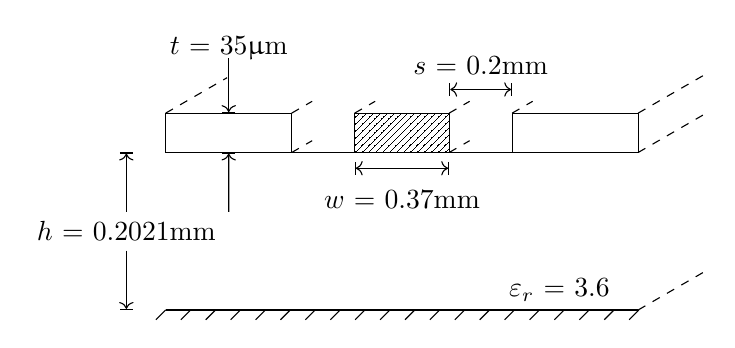
\begin{tikzpicture}
      \draw (0,0) node[name=sw]{} -- ++ (6,0) node[name=se]{};
      \draw[
          draw = none,
          decoration = {border, segment length=9, amplitude=5, angle = -135},
          postaction = {decorate, draw}
      ] (0,0) -- ++ (6.5,0);
      \draw (0, 2) node[name=nw]{} -- ++ (6, 0) node[name=ne]{};
      \draw (6, 2)[dashed] -- ++ (30: 1);
      \draw (6, 0)[dashed] -- ++ (30: 1);
      % Trace (Width = 1.2)
      \draw[pattern = flexible hatch] (2.4, 2) node[name=ms-sw]{} rectangle (3.6, 2.5) node[name=ms-ne]{};
      \draw (3.6, 2)[dashed] -- ++ (30: 0.3);
      \draw (2.4, 2.5)[dashed] -- ++ (30: 0.3);
      \draw (3.6, 2.5)[dashed] -- ++ (30: 0.3);
      % Coplanar GND (Width = 2.6)
      \draw (0, 2) rectangle ++ (1.6, 0.5);
      \draw (4.4, 2) rectangle ++ (1.6, 0.5);
      \draw (0, 2.5)[dashed] -- ++ (30: 0.9);
      \draw (6, 2.5)[dashed] -- ++ (30: 1);
      \draw (1.6, 2)[dashed] -- ++ (30: 0.3);
      \draw (1.6, 2.5)[dashed] -- ++ (30: 0.3);
      \draw (4.4, 2.5)[dashed] -- ++ (30: 0.3);
      % Gap (Width = 0.8)
      \draw (3.6, 2.8)[|<->|] -- (4.4, 2.8);
      \draw (4, 3.1) node{$s$ = 0.2mm};
      % Height
      \draw (-0.5, 1) node[name = height]{$h$ = 0.2021mm};
      \draw (height.north)[->|] -- (-0.5,2);
      \draw (height.south)[->|] -- (-0.5,0);
      % Width
      \draw (2.4, 1.8)[|<->|] -- (3.6, 1.8);
      \draw (3, 1.4) node{$w$ = 0.37mm};
      % Thickness
      \draw (height.north) ++ (1.3, 0)[->|] -- (0.8, 2);
      \draw (0.8, 2.5)[|<-] -- ++ (0, 0.7) node[name=t]{};
      \draw (t.north) node{$t$ = 35$\upmu$m};
      % Dielectric Constant
      \draw (5, 0.25) node[name = er]{$\varepsilon_r$ = 3.6};
    \end{tikzpicture}
  \end{center}
  \caption{Grounded Coplanar Waveguide Dimensions.}\label{fig:gcpw}
\end{figure}

The best-performing design as of date uses Mueller BU-1420761881 connectors with the footprint shown in Figure~\ref{fig:sma}. This footprint is also present in the repository, but the layer 2 ground cutout needs to be generated manually for each connector. The layer 1 ground cutout may also perform better with its right angles smoothed although the dimensions for this are not strict. Layers 3 and 4 are continuous ground planes. A grounded coplanar waveguide (Shown in Figure~\ref{fig:gcpw}) extends in a straight line from the SMA center conductor to the MMIC input pin. The dimensions were chosen as a compromise between ease of soldering components, where a larger trace width is better, and impedance matching the trace to MMIC pins, where a smaller trace width is better. As a result, only 0402 components will fit directly on the trace and SMA connectors with a center pin larger than 10 mils will likely incur problems.

For the best performance and stability, each RF trace should be fenced by two rows of plated through-hole vias on each side, with plenty of vias underneath and around MMIC components as well. One set of rows placed 1.2mm from the center of the trace with 1.2mm of via spacing, combined with another set of rows at 2.4mm from the center of the trace and the same via spacing worked well, however, the exact dimensions of this do not seem to be strict with the general rule of too many vias being preferable to not enough vias.

\colorlet{pcbcopper}{orange!30}
\colorlet{pcbother}{lightgray!30}
\colorlet{pcbother2}{cyan!25}
\begin{figure}
  \begin{center}
    \begin{tikzpicture}[z={(3.85mm, 6.5mm)}]
      \def\yfactor{0.75}
      \foreach \y in {0, 1, 2, 3} {\coordinate(ne\y) at (4.5, \yfactor*\y, 5);}
      \begin{scope}[canvas is xz plane at y=0]
        \draw(0, 0) node[anchor=north west, fill=pcbother2]{Layer 4};
        \draw(0, 0) [fill=pcbother]rectangle (ne0);
      \end{scope}
      \begin{scope}[canvas is xz plane at y=\yfactor*1]
        \draw(0, 0) node[anchor=north west, fill=pcbother2]{Layer 3};
        \draw(0, 0) [fill=pcbother]rectangle (ne1);
      \end{scope}
      \begin{scope}[canvas is xz plane at y=\yfactor*2]
        \draw(0, 0) node[anchor=north west, fill=pcbother2]{Layer 2};
        \draw(0, 0) [fill=pcbother]rectangle (ne2);
        \path(0, 0) -- coordinate[pos=0.5](midpointsouth) (current subpath start -| ne2);
        \draw([xshift=-0.35cm]midpointsouth) coordinate(rectanglesw) [fill=white]rectangle ++ (0.7, 2) coordinate(rectanglene);
      \end{scope}
      \begin{scope}[canvas is xz plane at y=\yfactor*3]
        \draw(0, 0) node[anchor=north west, fill=pcbother2]{Layer 1};
        \draw(0, 0) [fill=white]rectangle (ne3);
        \fill[pcbcopper](0, 0) -- (0, 5) -- (1.7, 5) -- (1.7, 2) -- (1.25, 2) -- (1.25, 0) -- cycle;
        \fill[pcbcopper](4.5, 0) -- (4.5, 5) -- (2.8, 5) -- (2.8, 2) -- (3.25, 2) -- (3.25, 0) -- cycle;
        \draw(0, 0) rectangle (ne3);
        \path(0, 0) -- coordinate[pos=0.5](midpointsouth) (current subpath start -| ne3);
        \draw([xshift=-1cm]midpointsouth) -- ++ (0, 2) -- ++ (0.45, 0) to (\tikztostart |- ne3);
        \draw([xshift=1cm]midpointsouth) -- ++ (0, 2) -- ++ (-0.45, 0) to (\tikztostart |- ne3);

        \draw([xshift=-0.25cm]midpointsouth) coordinate(tracesw) -- (current subpath start |- ne3);
        \draw([xshift=0.25cm]midpointsouth) -- (current subpath start |- ne3) coordinate(tracene);
        \fill[pcbcopper]([xshift=-0.25cm]midpointsouth) rectangle (tracene);
        \pgflowlevelsynccm % Makes arrows transform on plane but only works with explicit coords (no names)
        \draw[dotted](1.25, 2) -- ++ (-0.5, 0);
        \draw[<->|](0.75, 0) -- node[pos=0.5, fill=pcbcopper]{5.08} (0.75, 2);
        \draw[dotted](1.25, 2) -- ++ (0, 0.5);
        \draw[dotted](3.25, 2) -- ++ (0, 0.5);
        \draw[|<-](1.25, 2.5) -- ++ (-0.25, 0);
        \draw[|<-](3.25, 2.5) -- ++ (0.25, 0);
        \draw(3.5, 2.5) node[fill=pcbcopper, anchor=west]{1.41};
        \draw(2.25, 1) node[rotate=90]{\small Trace};
        \draw(2.25, 4) node[rotate=90]{\small Trace};
      \end{scope}

      \tikzset{xshift=7cm}
      \foreach \y in {0, 1, 2, 3} {\coordinate(ne\y) at (4.5, \yfactor*\y, 5);}
      \begin{scope}[canvas is xz plane at y=0]
        \draw(0, 0) node[anchor=north west, fill=pcbother2]{Layer 4};
        \draw(0, 0) [fill=pcbother]rectangle (ne0);
      \end{scope}
      \begin{scope}[canvas is xz plane at y=\yfactor*1]
        \draw(0, 0) node[anchor=north west, fill=pcbother2]{Layer 3};
        \draw(0, 0) [fill=pcbother]rectangle (ne1);
      \end{scope}
      \begin{scope}[canvas is xz plane at y=\yfactor*2]
        \draw(0, 0) node[anchor=north west, fill=pcbother2]{Layer 2};
        \draw(0, 0) [fill=pcbcopper]rectangle (ne2);
        \path(0, 0) -- coordinate[pos=0.5](midpointsouth) (current subpath start -| ne2);
        \draw([xshift=-0.35cm]midpointsouth) coordinate(rectanglesw) [fill=white]rectangle ++ (0.7, 2) coordinate(rectanglene);
        
        \draw[dotted](rectanglesw |- rectanglene) -- ++ (0, 0.5);
        \draw[dotted](rectanglene) -- ++ (0, 0.5);
        \pgflowlevelsynccm % Makes arrows transform on plane but only works with explicit coords (no names)
        \draw[<->|](1.4, 0) -- node[pos=0.5, fill=pcbcopper]{5.08} (1.4, 2);
        \draw[dotted](1.5, 2) -- (2, 2);
        \draw[|<->|](1.9, 2.5) -- (2.6, 2.5);
        \draw(2.25, 3) node[fill=pcbcopper]{0.5};
      \end{scope}
    \end{tikzpicture}
  \end{center}
  \caption{Ground Clearance Dimensions for SMA Landings in mm.}\label{fig:sma}
\end{figure}

\subsection{DRIFT Integration}\label{sec:drift}
The Dynamic Radio Interference Finding Tool (DRIFT) is an Electromagnetic Spectrum Management project intended to be an external-facing, web-based interface to visualize RFI data from various sites including VLA, GBT, VLBA, CHIME, ASM-2, and the RF-DFS/EMS.\@

Sweeps collected in \verb|AUTO| mode will also be automatically uploaded to the DRIFT database whereas \verb|MANUAL| sweeps can only be saved to the local machine. These sweeps are saved in a csv format that mimics those saved locally on the N9040B, containing lines of parameters with their values separated by commas as shown in Figure~\ref{fig:csvexample}.

\begin{figure}[ht]
\begin{lstlisting}[aboveskip=0pt, belowskip=0pt]
Trace,
Swept SA,
A.33.03,N9040B
Number of Points,1001
Sweep Time,0.020066667
Start Frequency,10000000
Stop Frequency,12000000000
\end{lstlisting}
\begin{lstlisting}[aboveskip=0pt, belowskip=0pt, numbers=none]
...
\end{lstlisting}
\begin{lstlisting}[aboveskip=0pt, belowskip=0pt, firstnumber=43]
X Axis Units,Hz
Y Axis Units,dBm
DATA
10000000,-71.1912847253302
21990000,-105.183861324451
33980000,-72.2399984094122
\end{lstlisting}
\begin{lstlisting}[aboveskip=0pt, belowskip=0pt, numbers=none]
...
\end{lstlisting}
\caption{Example Trace CSV.}\label{fig:csvexample}
\end{figure}

Note that these csv files are first converted to a file with a format compatible for DRIFT processing by removing extraneous data and performing frequency unit conversions to MHz. For the sake of consistency with DRIFT nomenclature, a \textit{scan} is equivalent to a spectrum analyzer sweep whereas a \textit{reading} refers to a single pair of x-y points. Table~\ref{tab:driftdata} shows what fields are stored by DRIFT;\@ all fields are assumed to be scan-level metadata unless otherwise specified.

\begin{table}[ht]\rowcolors{1}{lightgray!30}{white}
  \begin{center}
    \begin{tabularx}{\linewidth}{l|l|X}
      Field       & Required  & Description \\ \hline
      \lstinline|instrument|    & Yes & Unique identifier for instrument or device (VLA, VLBA-PT, VLBA-LA, RF-DFS, RF-EMS, etc.) per scan.\\
      \lstinline|receiver|      & Yes & DRIFT will have a separate list of receivers for each instrument (DFS1, EMS1, etc.). \\
      \lstinline|polarization|  & Yes & Hardcoded for NM spectrum monitoring devices (EMS is linear vertical, DFS is unknown.)\\
      \lstinline|intensity_unit|& Yes & Hardcoded for NM spectrum monitoring devices (dBm). \\
      \lstinline|scan_name|     & Yes & Unique string to represent the scan, will be displayed to the end user.\\
      \lstinline|scan_datetime| & Yes & One UTC time, isoformat, with timezone attached, to represent the entire scan.\\
      \lstinline|scan_az|       & No  & Where the device is pointed in decimal degrees, one value to represent the entire scan, not relevant for the EMS.\\
      \lstinline|scan_el|       & No  & Where the device is pointed in decimal degrees, one value to represent the entire scan, not relevant for the EMS.\\
      \lstinline|configuration| & No  & Selected from hardcoded list (VLA configurations, not relevant to NM spectrum monitoring devices).\\
      \lstinline|instrument_lat|& No  & ASM-2 devices only, other instruments have their locations hardcoded.\\
      \lstinline|instrument_long|&No  & ASM-2 devices only, other instruments have their locations hardcoded.\\
      \lstinline|frequency|     & Yes & Primary independent variable (reading-level), supplied in MHz.\\
      \lstinline|intensity|     & Yes & Primary dependent variable (reading-level), supplied in \lstinline|intensity_unit|.\\
      \lstinline|reading_az|    & No  & Azimuth for a specific reading in decimal degrees (ASM-2 only).\\
      \lstinline|reading_el|    & No  & Elevation for a specific reading in decimal degrees (ASM-2 only).\\
    \end{tabularx}
  \end{center}
  \caption{DRIFT Unified Fields. Not all fields are used by all sites.}\label{tab:driftdata}
\end{table}\rowcolors{1}{white}{white}

DRIFT's upload format requires that csv files have their top row populated with the fields relevant to the given site, followed by a row of values or multiple rows in the case of reading-specific metadata. See Figure~\ref{fig:driftcsvexample} for an example of a csv that would be uploaded to DRIFT.\@ DRIFT does not save these files for a substantial amount of time once they are processed and neither does \verb|EMSMONPC2|. They are converted from the trace format in Figure~\ref{fig:csvexample} to the DRIFT compatible format in Figure~\ref{fig:driftcsvexample}, then uploaded. The Python script which handles this conversion will regularly clean these cached files at an arbitrary time interval. Additionally, DRIFT assumes that if a file with the same \verb|scan_name| is uploaded twice, then the initial table linked to \verb|scan_name| should be replaced. Because of this, it is imperative that scan names are not changed and contain at least a date and an iterating integer for that day.

\begin{figure}[ht]
\begin{lstlisting}[aboveskip=0pt, belowskip=0pt]
instrument,receiver,polarization,intensity_unit,scan_name,scan_datetime,frequency,intensity
ems,ems1,l,dbm,ems1-2025-03-28-0002,2025-03-28T11:49:55.199981+00:00,10000000,-71.1912847253302
,,,,,,21990000,-105.183861324451
,,,,,,33980000,-72.2399984094122
\end{lstlisting}
\begin{lstlisting}[aboveskip=0pt, belowskip=0pt, numbers=none]
...
\end{lstlisting}
\caption{Example DRIFT Upload CSV.}\label{fig:driftcsvexample}
\end{figure}

\subsection{RF-EMS Conduit Diagram}
Figure~\ref{fig:oldems} shows two diagrams of the EMS lightning protection system from the 2001 NMT Senior Design report of the EMS (VLA/VLBA Interference Memo \#19). This iteration had some notable differences such as an azimuth and elevation rotator, serial control lines, and metal-oxide varistors for lightning protection. None of these are used in this upgrade project but the diagrams may still be useful for characterizing conduit lines. Note that STS refers to the previous name for the RF-DFS - the Satellite Tracking System.
\begin{figure}[!ht]
  \begin{center}
    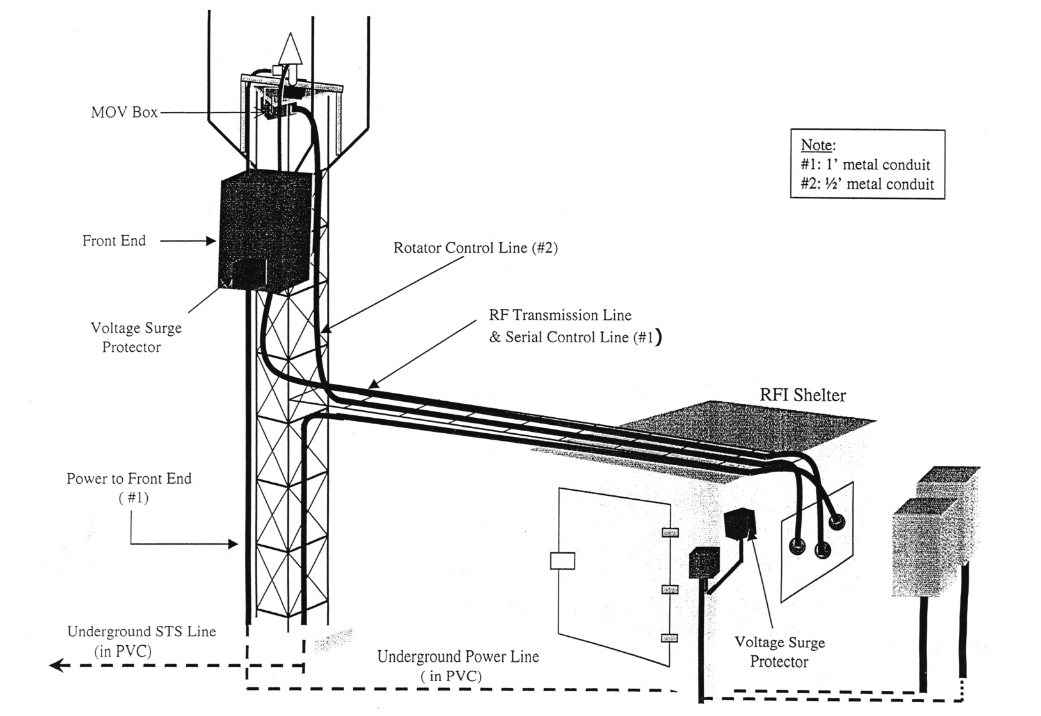
\includegraphics[width=0.8\textwidth]{images/oldems.png}
    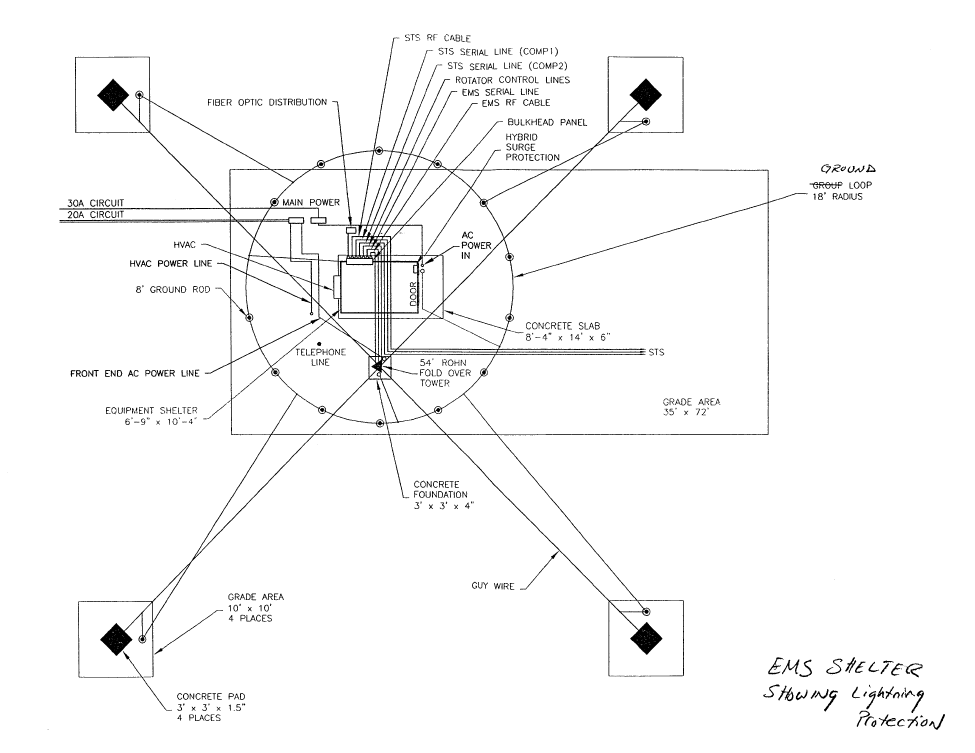
\includegraphics[width=\textwidth]{images/oldems2.png}
  \end{center}
  \caption{2001 RF-EMS Lightning Protection System.}\label{fig:oldems}
\end{figure}

\end{document}


